\chapter{Chapter 3}

\section{Problem definition}
\label{chpt: Problem definition}
In this work we expand on the results presented in \cite{centofanti2024comconf}, and developed in \cite{centofanti2024cma} and \cite{pellegrini2025mlcse}. In these articles an operator learning architecture (with a particular focus on FNO \footnote{see section ...}) has been used to learn the dynamics of a neuronal system, described by a ionic model (the FitzHugh-Nagumo or Hudgin-Huxely model \footnote{see section ...}). 
First of all the reaction has been simulated numerically by solving the underlying stiff systems of ordinary differential equations (ODEs). In the earlier works \cite{centofanti2024comconf, centofanti2024cma}, the MATLAB routine \texttt{ode15s} was utilized to integrate the equations over a fixed timespan (e.g., 100 ms) and the solutions were sampled on a uniform equispaced grid of 500 points. In the most recent development \cite{pellegrini2025mlcse}, which extends the study to higher-dimensional systems like the O'Hara-Rudy model, a Runge-Kutta method was employed. In all cases, the systems were perturbed using time-dependent applied currents, typically in the form of square pulses with varying intensities and durations, to explore the threshold-dependent dynamics and complex oscillatory behaviors of the cells.

The numerical solutions were then collected to construct the datasets for the operator learning task. Specifically, in the initial studies on the FitzHugh-Nagumo and Hodgkin-Huxley models, the authors generated a total of 2000 trajectories, split into 1600 samples for the training set and 400 for the test set \cite{centofanti2024comconf, centofanti2024cma}. Subsequently, to handle the increased complexity and ensure comprehensive coverage of the dynamical behaviors in higher-dimensional spaces, the dataset size was expanded to a total of 3750 trajectories, comprising 3000 training examples, 375 for validation, and 375 for testing \cite{pellegrini2025mlcse}.

Using these datasets, a Fourier Neural Operator (FNO) was trained to learn the non-linear mapping from the applied input current to the system's state variables (i.e., transmembrane potential, recovery, and gating variables). By leveraging the Fast Fourier Transform (FFT) on the uniform discretization grid, the FNO architecture computes the integral kernel operator directly in the frequency domain. This approach proved highly effective in capturing the global dependencies and multiscale temporal behaviors of the stiff ionic models, maintaining stable training and achieving very low relative $L^2$ errors across all the investigated dimensionalities.

The results across these studies demonstrate that FNOs are highly effective in learning the dynamics of stiff ionic models, consistently achieving low relative $L^2$ errors. Specifically, the optimized FNO architectures attained test errors of approximately 2.0\% for the FitzHugh-Nagumo model \cite{centofanti2024comconf}, 1.4\% for the Hodgkin-Huxley model \cite{centofanti2024cma}, and around 2.0\% even for the highly complex 41-variable O'Hara-Rudy model \cite{pellegrini2025mlcse}. Furthermore, the most recent findings emphasize the remarkable scalability of this approach: despite the substantial increase in system dimensionality, properly tuned FNOs maintain bounded training and test errors, with memory usage and training time scaling only linearly \cite{pellegrini2025mlcse}. This confirms the capability of FNOs to accurately and efficiently capture complex multiscale electrophysiological dynamics, gracefully overcoming the curse of dimensionality that typically affects artificial neural networks in high-dimensional settings.

% Versione senza "curse of dimensionality"
%This confirms the capability of FNOs to accurately and efficiently capture complex multiscale electrophysiological dynamics, exhibiting a linear scaling of memory and training time with respect to the system's dimensionality, while maintaining bounded parameters and relative errors \cite{pellegrini2025mlcse}.


\begin{figure}[htbp]
    \centering
    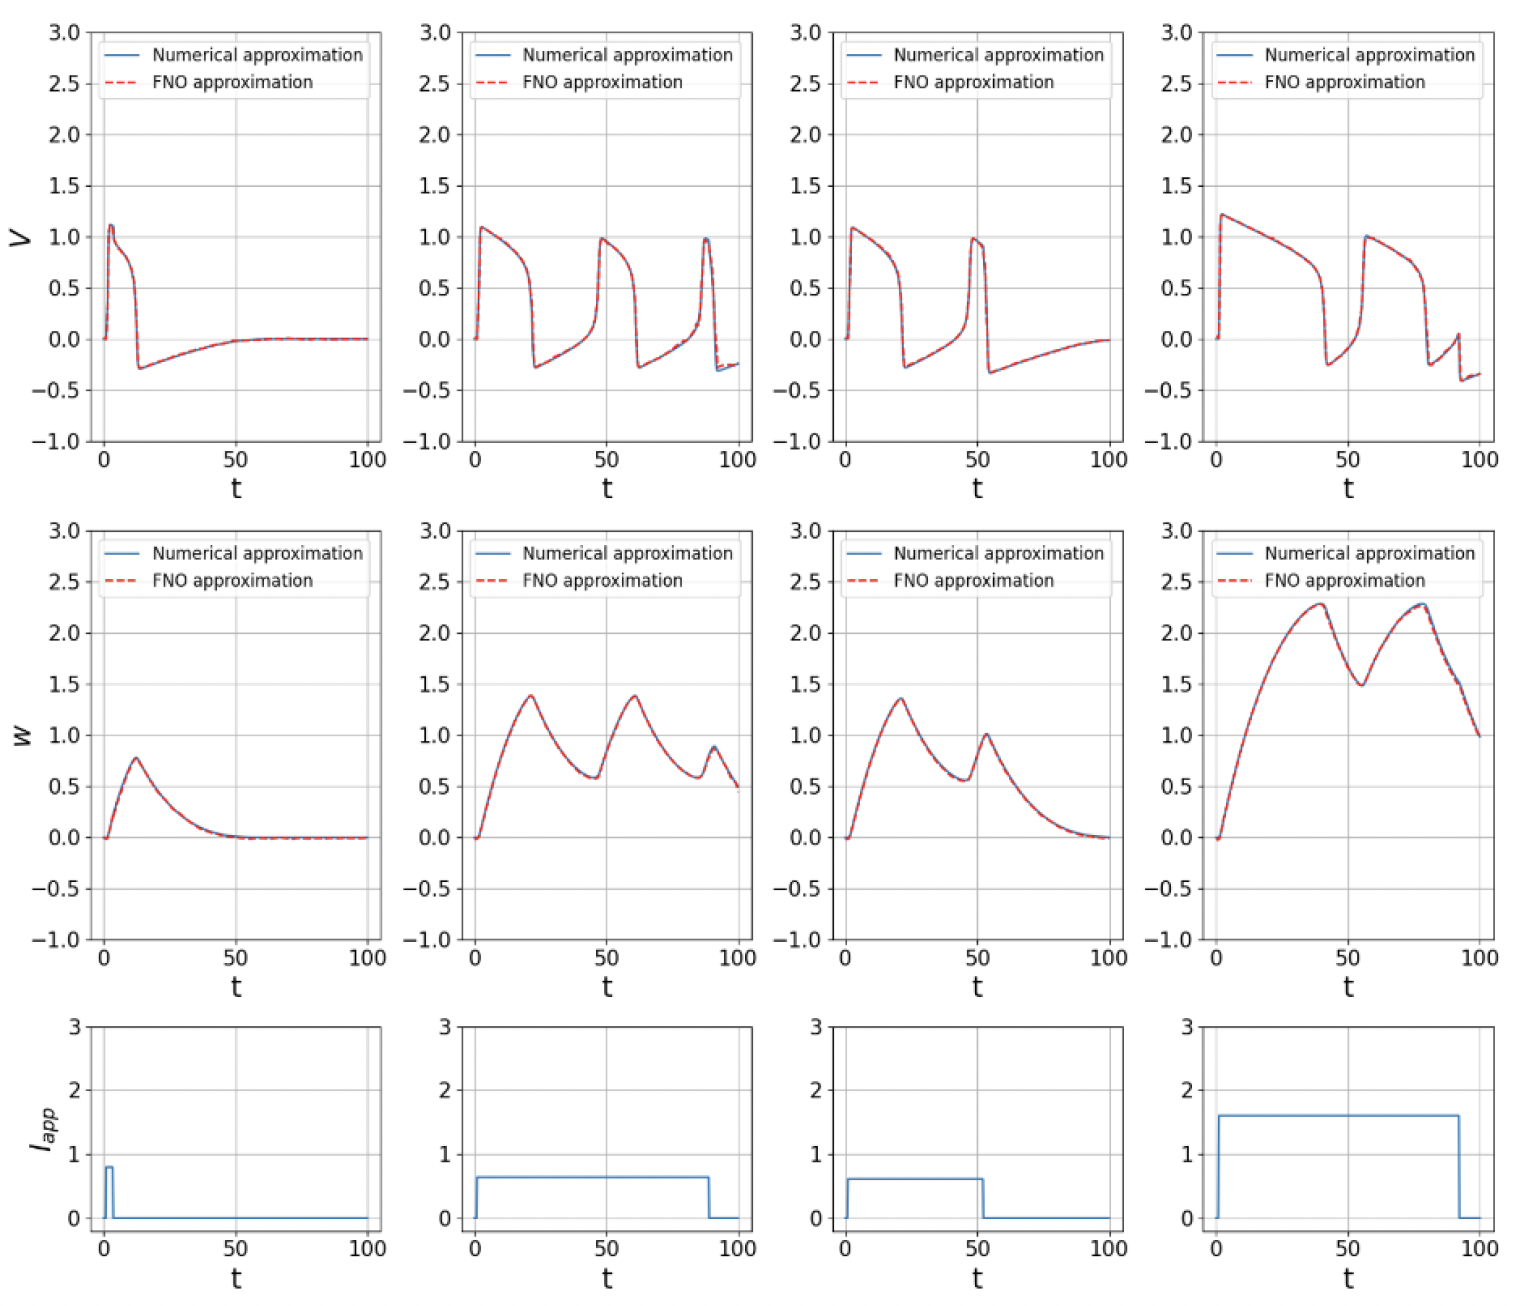
\includegraphics[width=0.55\textwidth]{img/FH_model/No_Network/Centofanti_article_figure.png}
    \caption{Numerical and FNO approximations in four tests (one per column): output potential $V$ (top), output recovery variable $w$ (center) and corresponding input current $I_{app}$ (bottom).}
    \label{fig:centofanti_dynamics}
\end{figure}

\newpage
\section{From single neuron to spatially extended systems}
However, the setup considered is that of a single node.
We generalized this approach by analyzing a spatial extended system: a current (in the form of square wave) is given as input to an \textcolor{blue}{\textbf{input node}}, information is transmitted through diffusion (where each node has a local reaction term following FitzHugh-Nagumo, see eq \eqref{eq:coupled_FHN}), and the potential is read/ predicted by the NN for the \textcolor{red}{\textbf{output node}}.


\begin{figure}[htbp]
    \centering
    % --- Prima immagine (sinistra) ---
    \begin{subfigure}[b]{0.48 \textwidth}
        \centering
        
\includegraphics[width=\textwidth]{img/FH_model/1to2/output0to1.png}
        \caption{Input $\rightarrow$ Output}
        \label{fig:fh_output}
    \end{subfigure}
    \hfill % <--- Questo inserisce uno spazio elastico tra le due immagini
    % --- Seconda immagine (destra) ---
    \begin{subfigure}[b]{0.48\textwidth}
        \centering
        
\includegraphics[width=\textwidth]{img/FH_model/Simple_cycle/dynamics_cycle.png}
        \caption{Input $\rightarrow$ Network $\rightarrow$ Output}
        \label{fig:fh_dynamics}
    \end{subfigure}
    
    % Didascalia principale e label per l'intera figura
    \caption{Examples of our setup}
    \label{fig:fh_comparison}
\end{figure}


%%%

Our system is described by the following set of equations on a graph $\mathcal{G} = (\mathcal{V}, \mathcal{E})$:
\begin{equation}
\label{eq:coupled_FHN}
\begin{aligned}
\frac{dV_i}{dt} &= b V_i (V_i - \beta)(\delta - V_i) - c w_i + I_{app, i}(t) - \sigma \sum_{j=1}^{|\mathcal{V}|} L_{ij} V_j \\
\frac{dw_i}{dt} &= \epsilon (V_i - \gamma w_i)
\end{aligned}
\end{equation}

Where the parameters are $b = 5$, $c = 1$, $\beta = 0.1$, $\delta = 1$, $\epsilon = 0.1$, $\gamma = 0.25$, as in \cite{centofanti2024comconf} and $i \in \{1, \dots, |\mathcal{V}|\}$ represents the node of interest.

The coupling term is expressed through the elements $L_{ij}$ of the graph Laplacian matrix, defined as $\mathbf{L} = \mathbf{D}_{deg} - \mathbf{A}$, where $\mathbf{D}_{deg}$ is the diagonal degree matrix and $\mathbf{A}$ is the adjacency matrix. Explicitly \footnote{We assume that the graph is unweighted}:
\begin{equation}
L_{ij} = 
\begin{cases} 
\text{deg}(i) & \text{if } i = j \\
-1 & \text{if } (i,j) \in \mathcal{E} \\
0 & \text{otherwise}
\end{cases}
\end{equation}
The coefficient $\sigma$ modulates the global intensity of diffusion across the network.

\newpage

%%%%
%Ci vuole un capitolo di spiegazione tecnica di come ho trainato FNO in questo setup?
%%%

\section{Training procedure}


\section{Study of different topologies}
We will now discuss the result across different "hidden" \footnote{The FNO architecture doesn't recieve any information about them} networks structures.


Please note the setup is the following \footnote{Unless otherwise specified}: the \textcolor{blue}{\textbf{input node}} is connected by a direct link to a random node of a network. The hidden network is simple \footnote{Devo spiegare undirected + unweighted ?}. Finally another random node is connected by another direct link to the \textcolor{red}{\textbf{output node}}.





\subsection{No network}
This is the first step for spatial extension of the setup of section \ref{chpt: Problem definition} (see fig. \ref{fig:fh_output}). 

To evaluate the performance of our Fourier Neural Operator in this extended configuration, we analyzed both the global error metrics (MSE\footnote{even if the authors of \cite{centofanti2024comconf} used relative $L^2$ errors, we preferred to use an absolute metric to avoid exploding gradients when the solution approaches the equilibrium point at $0$}) and (qualitatively) the network's ability to accurately capture the threshold dynamics. Figure \ref{fig:1to2_peaks} illustrates some instances of the test set. We can clearly see that the network was able to correctly predict the action potential peaks for the vast majority of the test samples, which is a crucial requirement for excitable models.

Furthermore, the training process exhibits stable convergence without signs of overfitting, as depicted by the training and test loss curves in Figure \ref{fig:1to2_performance}a. Finally, Figure \ref{fig:1to2_performance}b reports the distribution of the MSE error evaluated across the test set. The histogram confirms that the network maintains a highly concentrated and low error profile, proving that the operator learning approach remains robust and reliable even in this first spatial extension step.

% --- Figura singola (Picchi) ---
\begin{figure}[htbp]
    \centering
    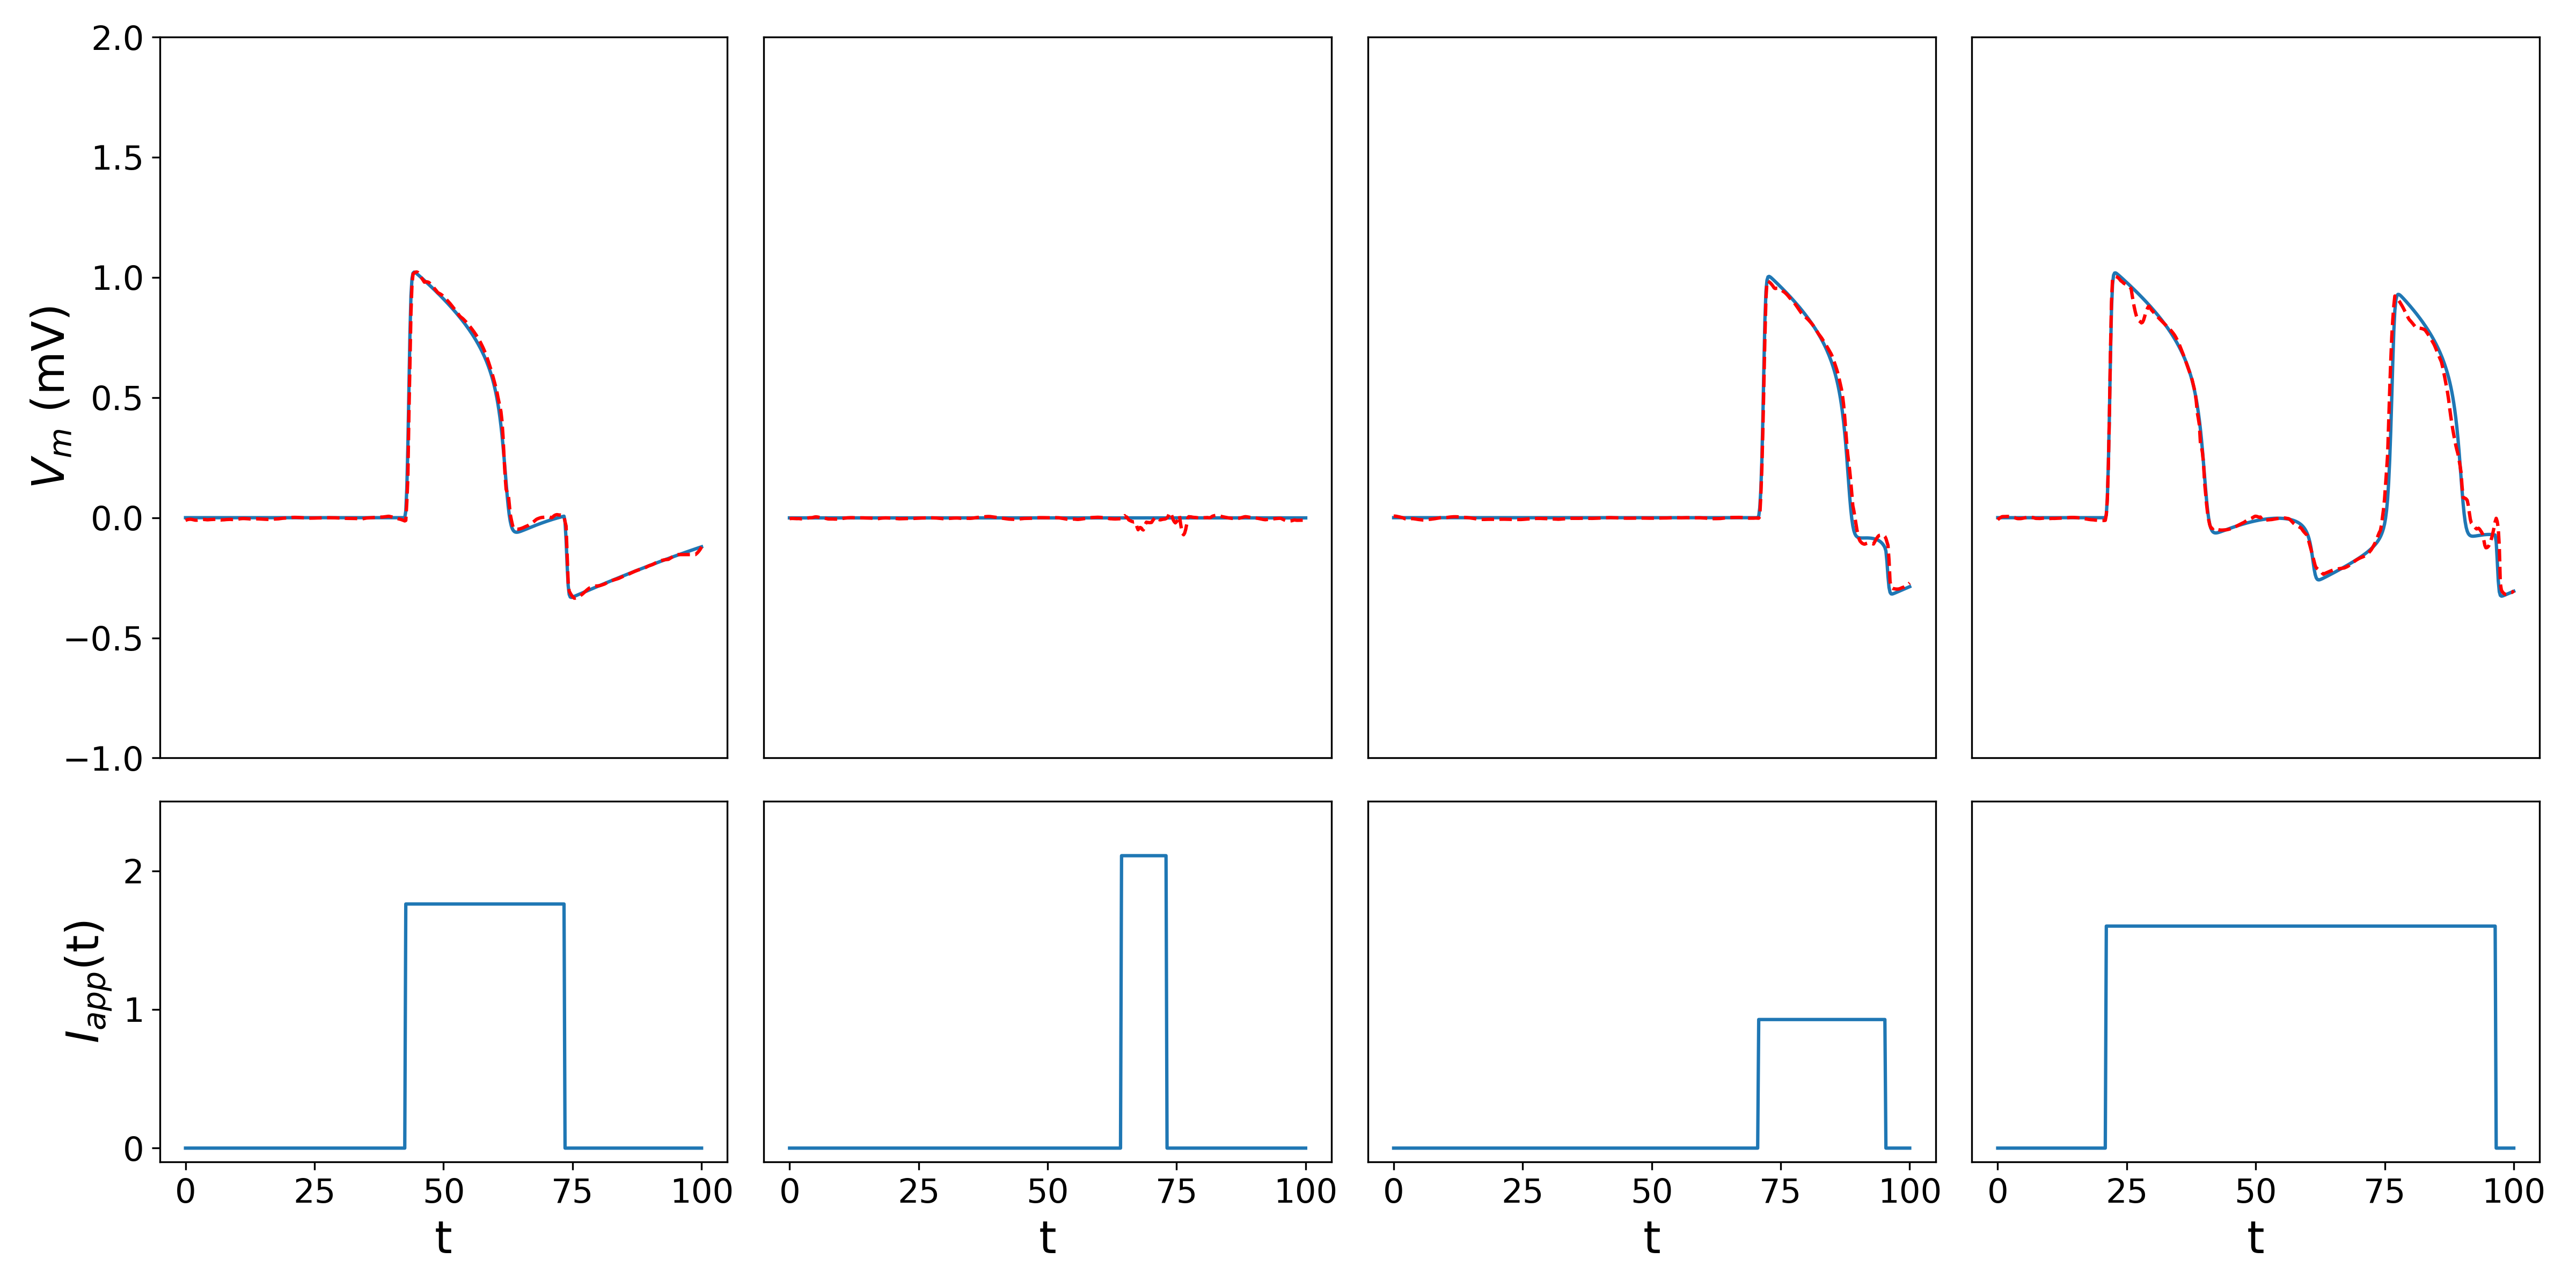
\includegraphics[width=0.7\textwidth]{img/FH_model/1to2/HHpeaks.png}
    \caption{Four instances of the test set. For each column we can see the Input current (bottom) with its corresponding potential response (top): the blue line represents the result of the simulations, whereas the dotted red line indicates the output of the NN}
    \label{fig:1to2_peaks}
\end{figure}

% --- Due figure affiancate (Loss e Istogramma L2) ---
\begin{figure}[htbp]
    \centering
    \begin{subfigure}[b]{0.48\textwidth}
        \centering
        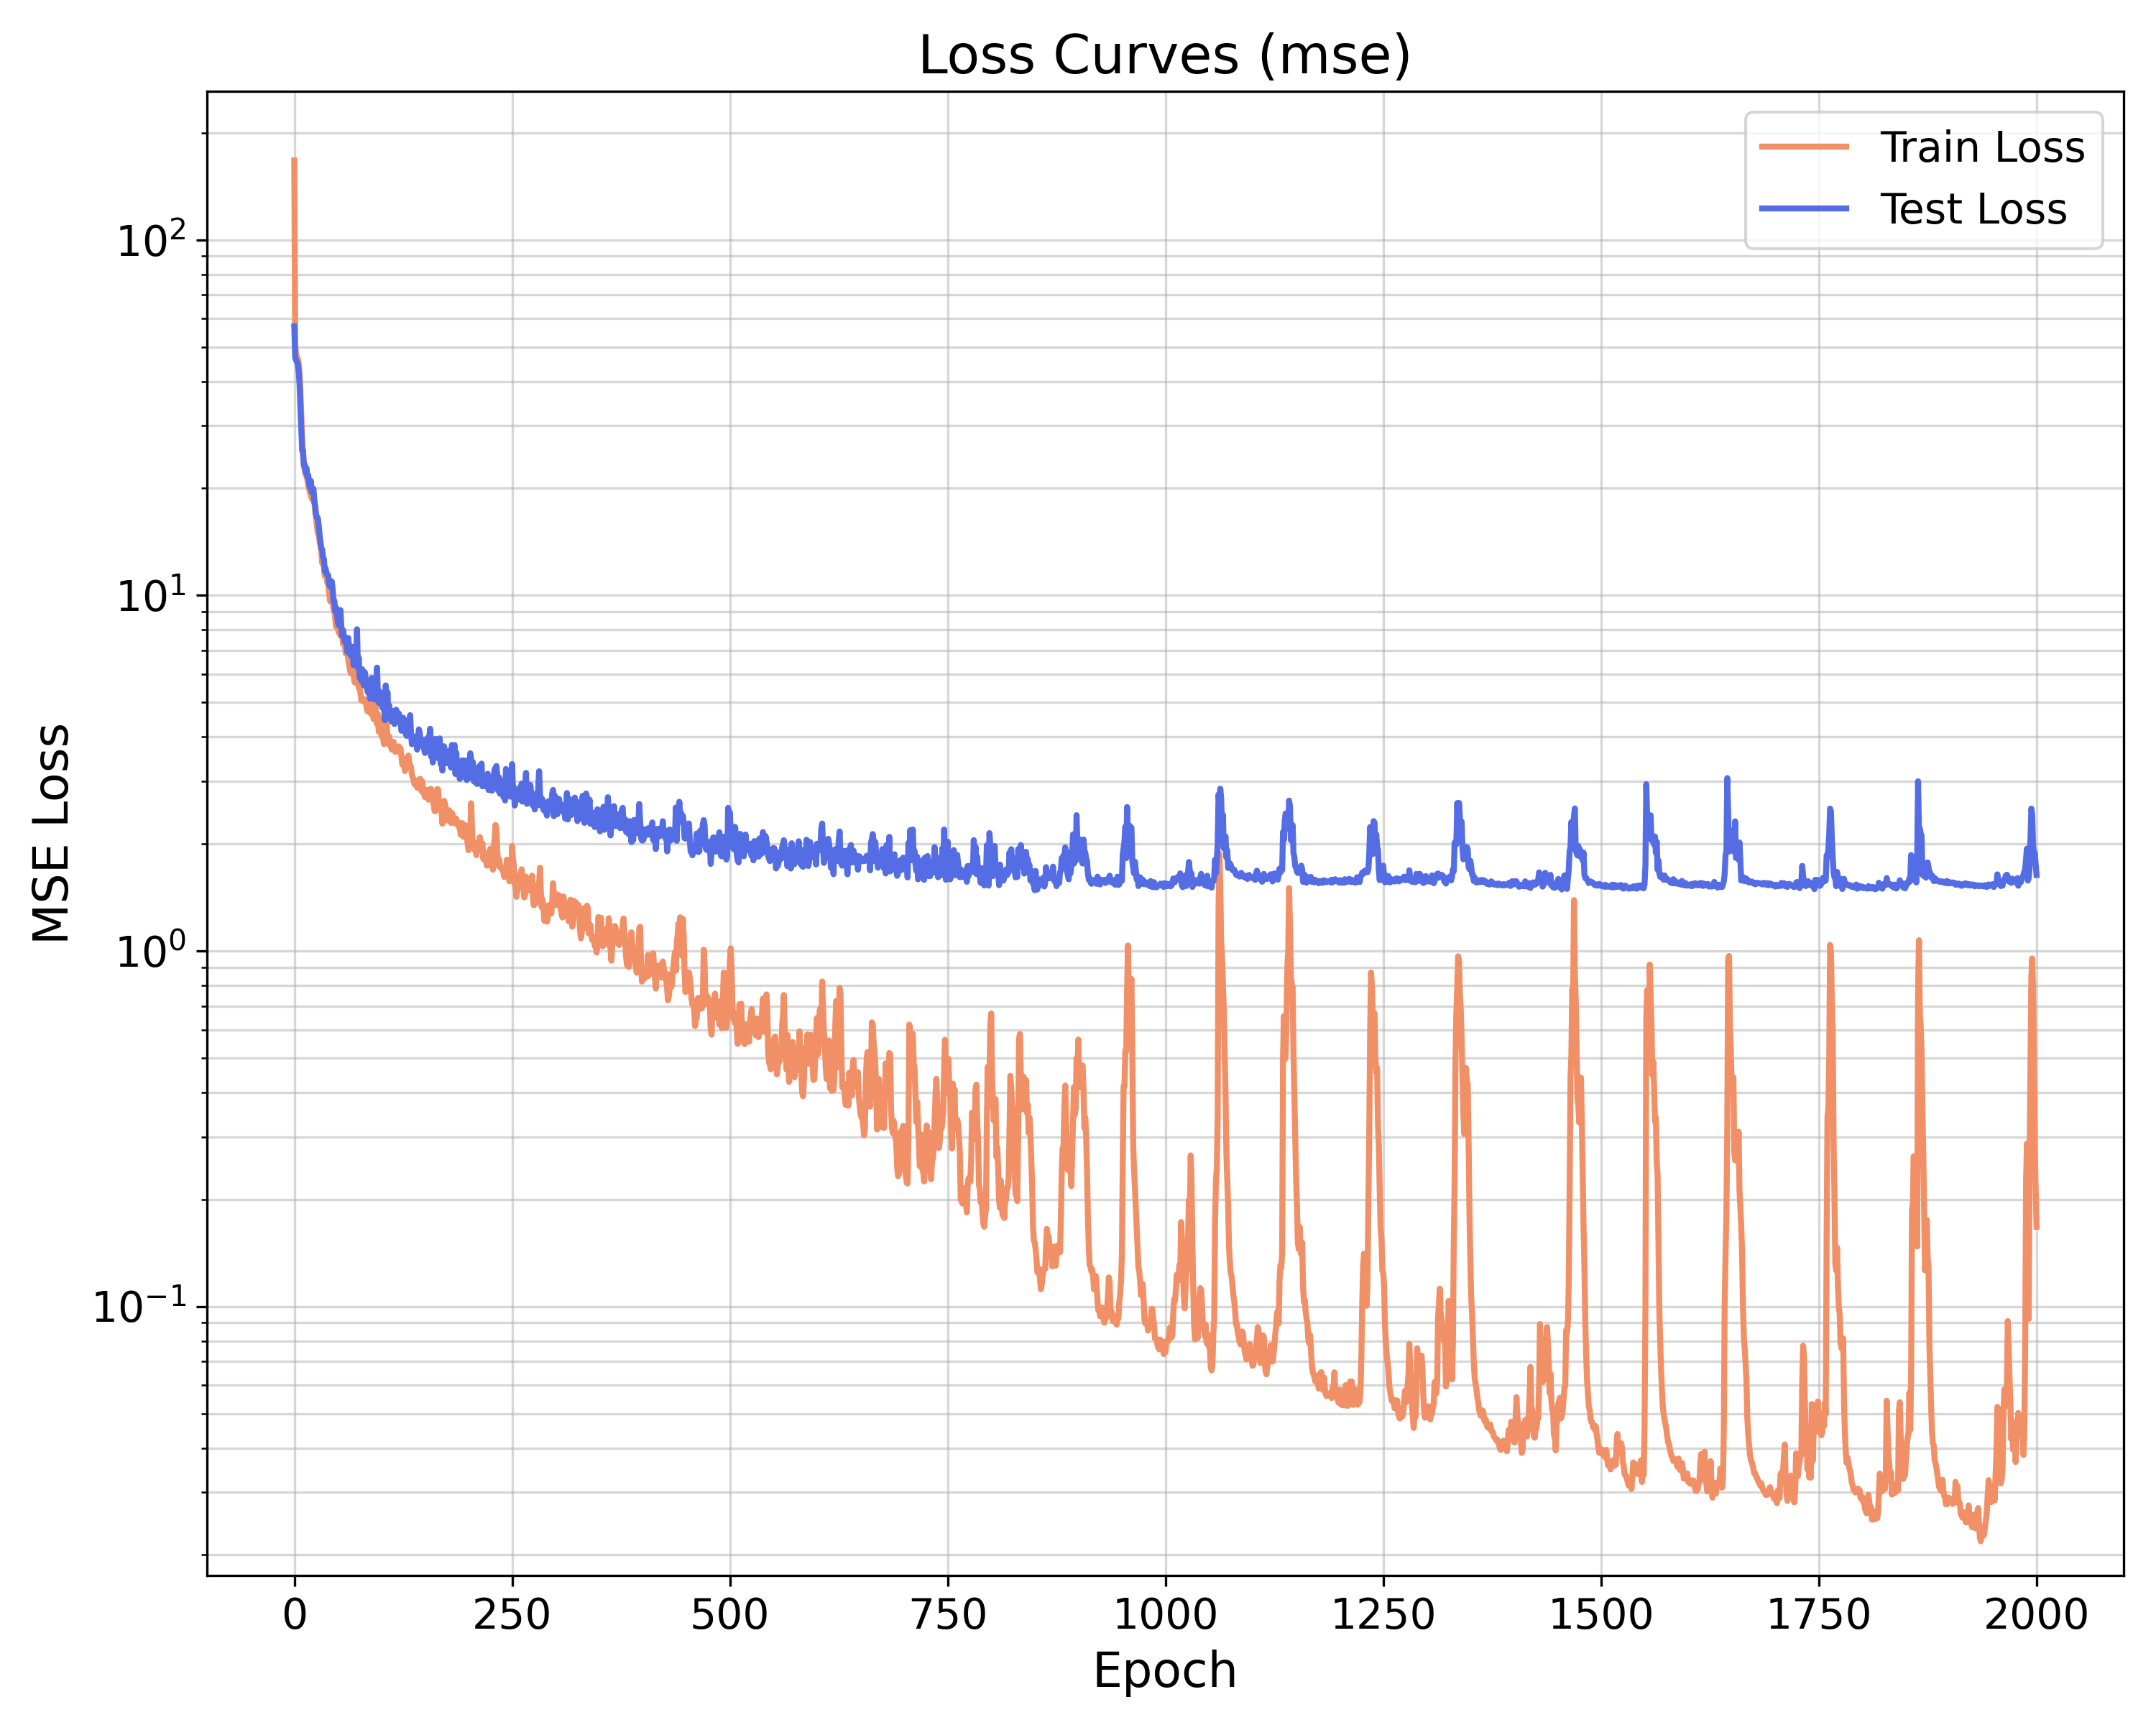
\includegraphics[width=\textwidth]{img/FH_model/1to2/loss_plot_fixed.png}
        \caption{Training and test loss}
        \label{fig:1to2_loss}
    \end{subfigure}
    \hfill
    \begin{subfigure}[b]{0.48\textwidth}
        \centering
        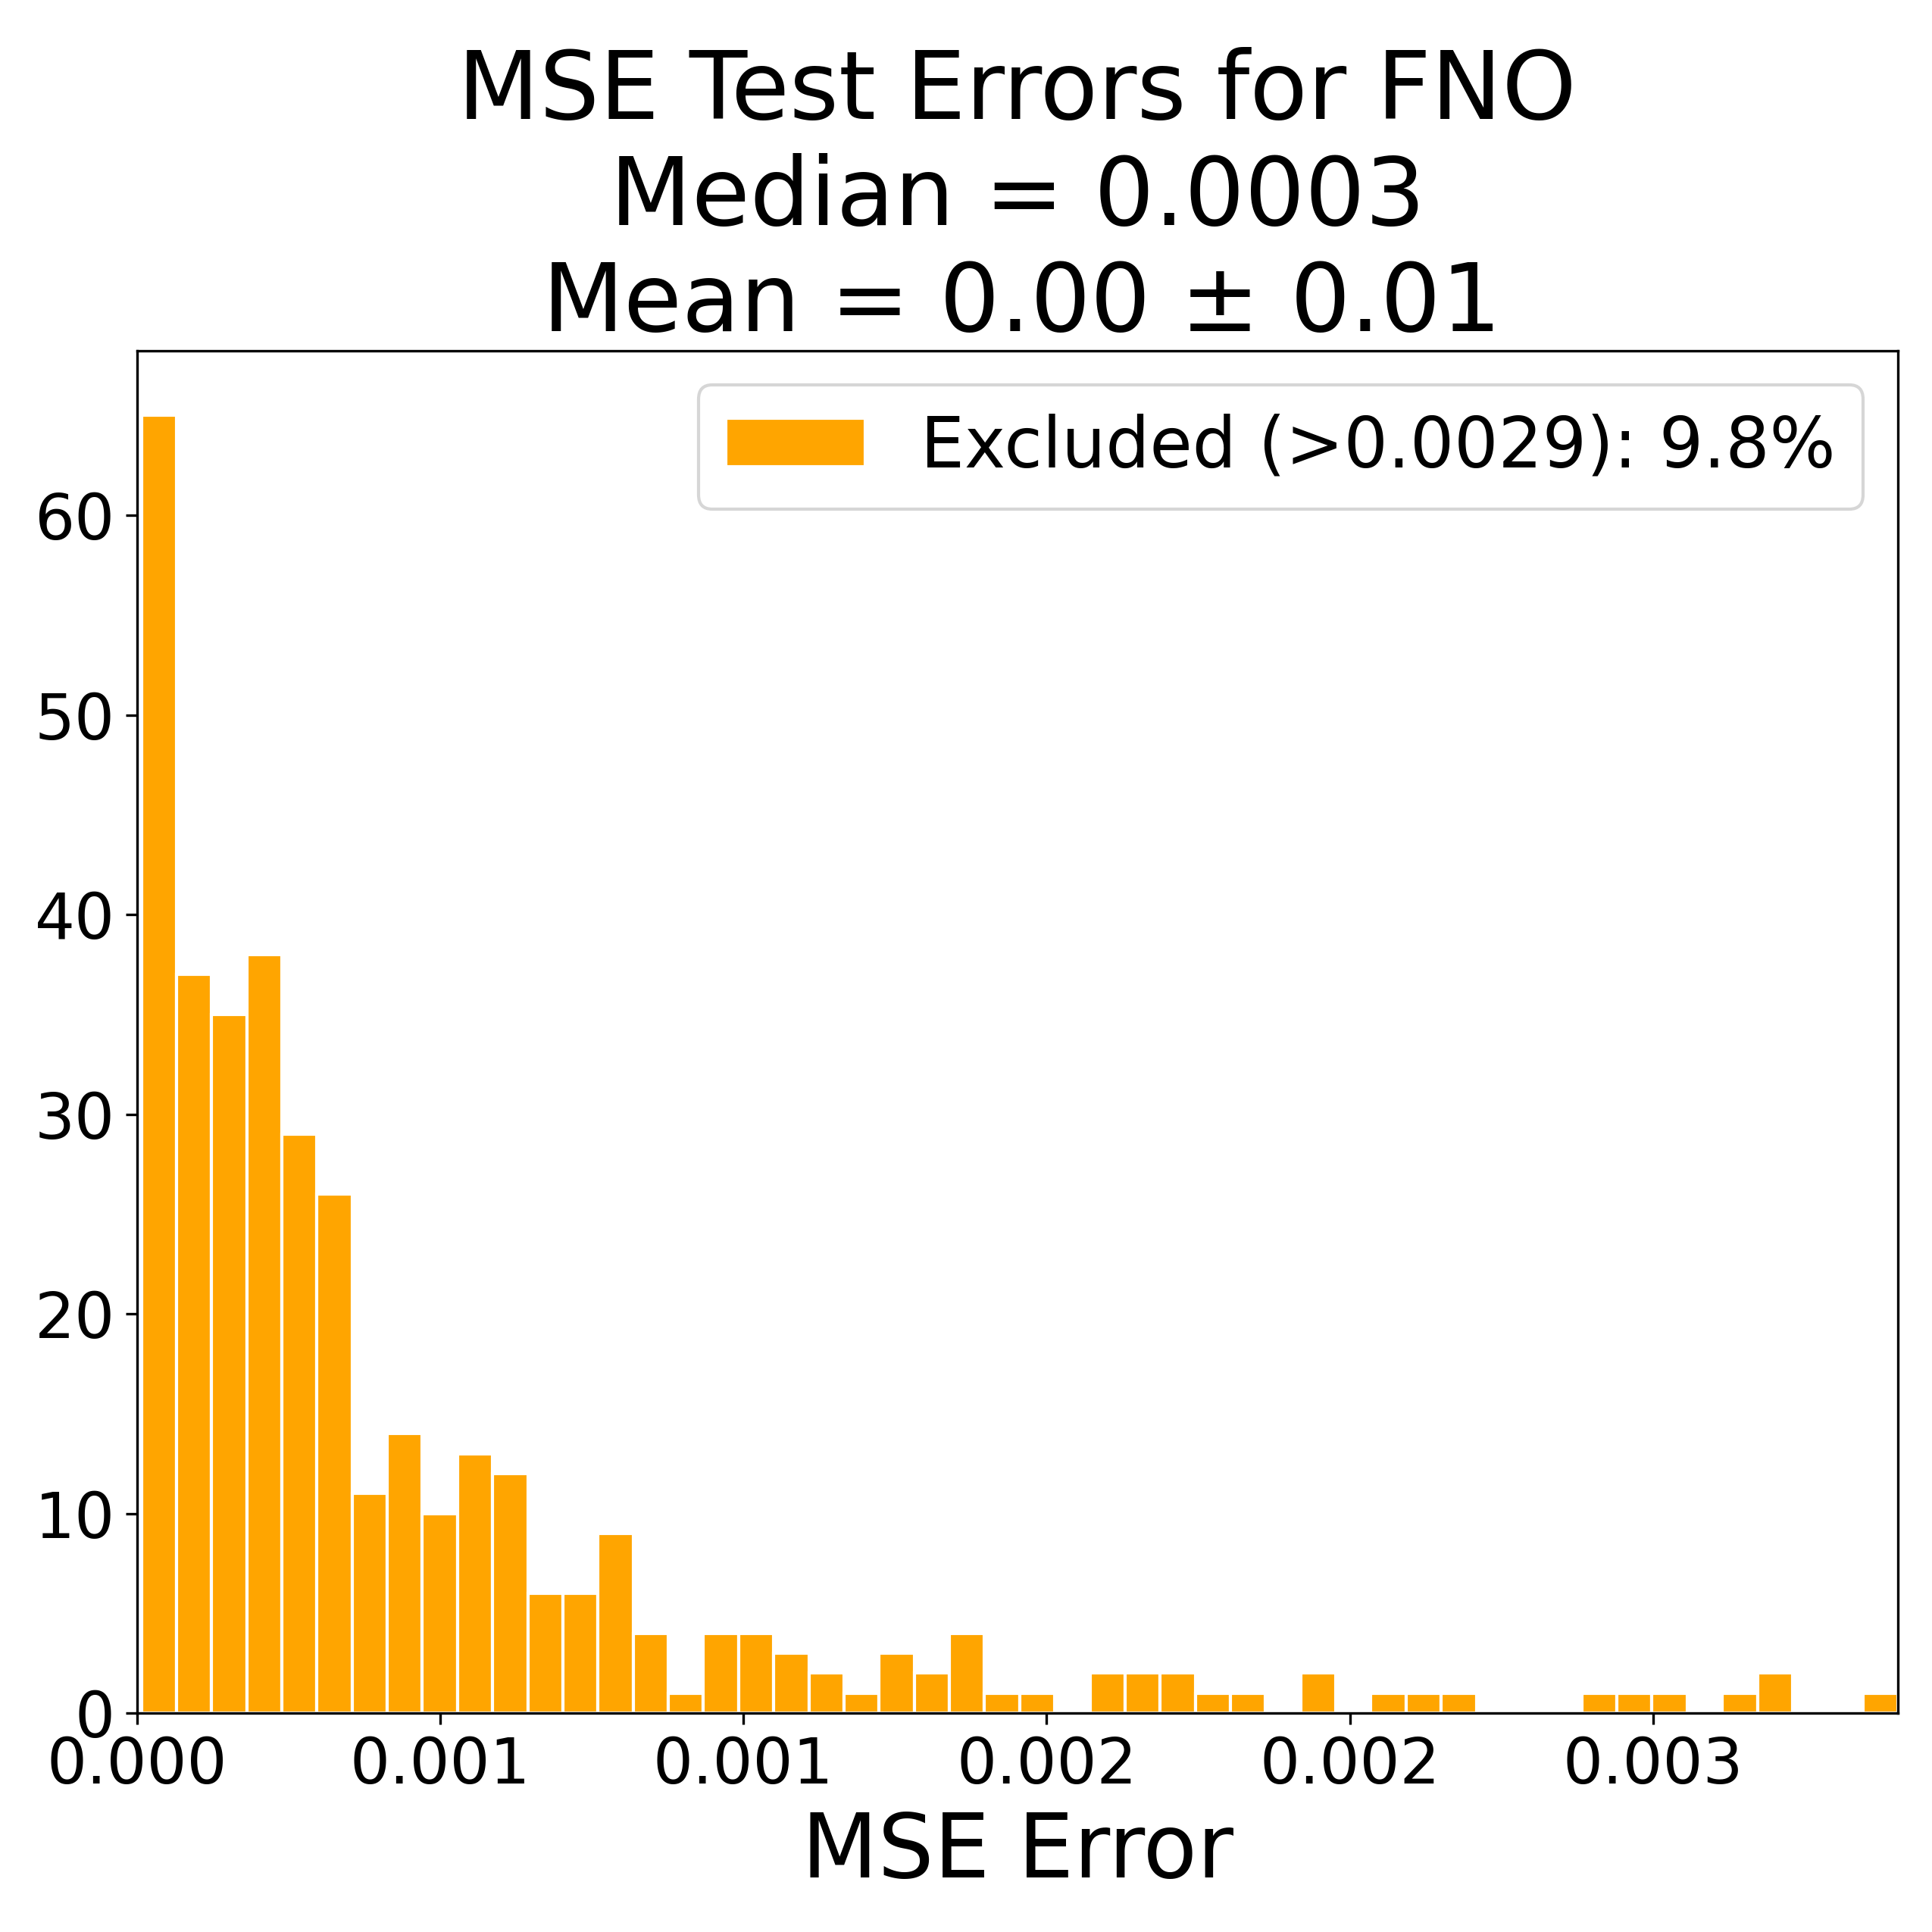
\includegraphics[width=\textwidth]{img/FH_model/1to2/L2histoFNO.png}
        \caption{MSE error distribution}
        \label{fig:1to2_l2histo}
    \end{subfigure}
    
    \caption{Loss convergence during the training process (a) and histogram of the MSE errors evaluated on the test set (b).}
    \label{fig:1to2_performance}
\end{figure}

\subsection{Toy network}
Following the same approach, we evaluated the FNO performance on a more complex spatial configuration, introducing a simple cycle topology (see fig. \ref{fig:fh_dynamics}). 

Consistent with the findings of the previous section, the network proves to be highly capable of capturing the underlying threshold dynamics. Figure \ref{fig:cycle_peaks} illustrates some instances of the test set for this new configuration. As we can see, the predicted dynamics strictly follow the numerical simulations, successfully reproducing the spiking behavior and the delay introduced by the diffusion over the cycle.

The global error metrics exhibit a behavior analogous to the "no network" scenario. As shown in Figure \ref{fig:cycle_performance}a, the training and test loss converge smoothly without any signs of overfitting. Furthermore, the MSE distribution across the test set (Figure \ref{fig:cycle_performance}b) remains tightly concentrated at very low values. This confirms that the operator learning approach is robust and its accuracy does not degrade when dealing with a small ($4$ nodes) network diffusion.

% --- Figura singola (Picchi Ciclo) ---
\begin{figure}[htbp]
    \centering
    
\includegraphics[width=0.7\textwidth]{img/FH_model/Simple_cycle/HHpeaks.png}
    \caption{Four instances of the test set for the simple cycle configuration. For each column we can see the applied input current (bottom) with its corresponding potential response (top): the blue line represents the result of the simulations, whereas the dotted red line indicates the output of the NN.}
    \label{fig:cycle_peaks}
\end{figure}

% --- Due figure affiancate (Loss e Istogramma Ciclo) ---
\begin{figure}[htbp]
    \centering
    \begin{subfigure}[b]{0.48\textwidth}
        \centering
        
\includegraphics[width=\textwidth]{img/FH_model/Simple_cycle/loss_plot_fixed.png}
        \caption{Training and test loss}
        \label{fig:cycle_loss}
    \end{subfigure}
    \hfill
    \begin{subfigure}[b]{0.48\textwidth}
        \centering
        
\includegraphics[width=\textwidth]{img/FH_model/Simple_cycle/L2histoFNO.png}
        \caption{MSE error distribution}
        \label{fig:cycle_l2histo}
    \end{subfigure}
    
    \caption{Loss convergence during the training process (a) and histogram of the MSE errors evaluated on the test set (b) for the simple cycle setup.}
    \label{fig:cycle_performance}
\end{figure}

\newpage
\subsection{ER network}
%devo fare un paragrafo in cui spiego cos'è l'ER network?
We proceeded with the study of larger networks. In particular, we wanted to observe if the performance of FNO degraded with the growing size ($N$) of the hidden network.
To conduct this experiment we performed our analysis for different size of the ER network $N= 10,100,200,300,400,500,600,700,800,900,1000,2000$ (with connection probability $p = \frac{3}{N}$).
Since the connection node for the input and output node are randomly chosen we repeated each experiments with different seeds $=0,42,100$ to distinguish if some effects are only due to chance of the particular topology/ sample of input/ output.

Here we reported only figures for the seed$=0$.

As a representative example of the system's behavior, Figure \ref{fig:er_setup_100} reports the potential dynamics for a network of size $N=100$ generated with seed $100$.

\begin{figure}[htbp]
    \centering
    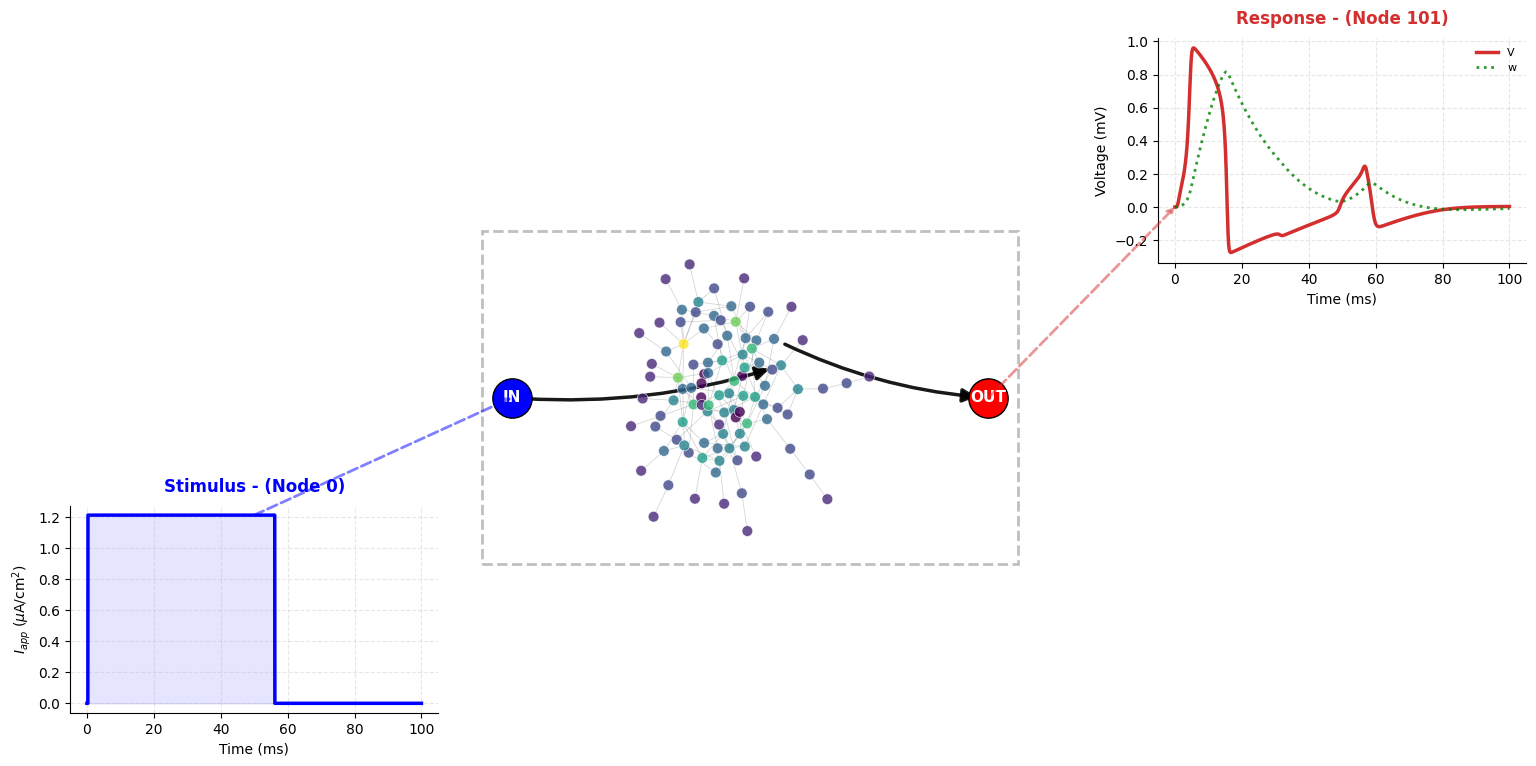
\includegraphics[width=\textwidth]{img/FH_model/ER_Network/dynamics_network_ER_N=100_seed=42.png}
    \caption{Our setup for an Erd\H{o}s-R\'enyi network of size $N=100$ (seed $100$)}
    \label{fig:er_setup_100}
\end{figure}

%%%
To systematically evaluate the threshold dynamics across all network dimensions, Figure \ref{fig:er_peaks_grid} reports the error distribution regarding the predicted number of action potential peaks for each size $N$. As we can observe from this comprehensive grid, the FNO robustly maintains its high accuracy: the vast majority of test instances exhibit zero error in the spike count, regardless of the significant increase in the network dimensionality. This confirms that the model's ability to capture the exact spiking behavior is not compromised by the growing scale of the spatial diffusion.

\begin{figure}[htbp]
    \centering
    % --- Prima riga ---
    \begin{subfigure}[b]{0.32\textwidth}
        \centering
        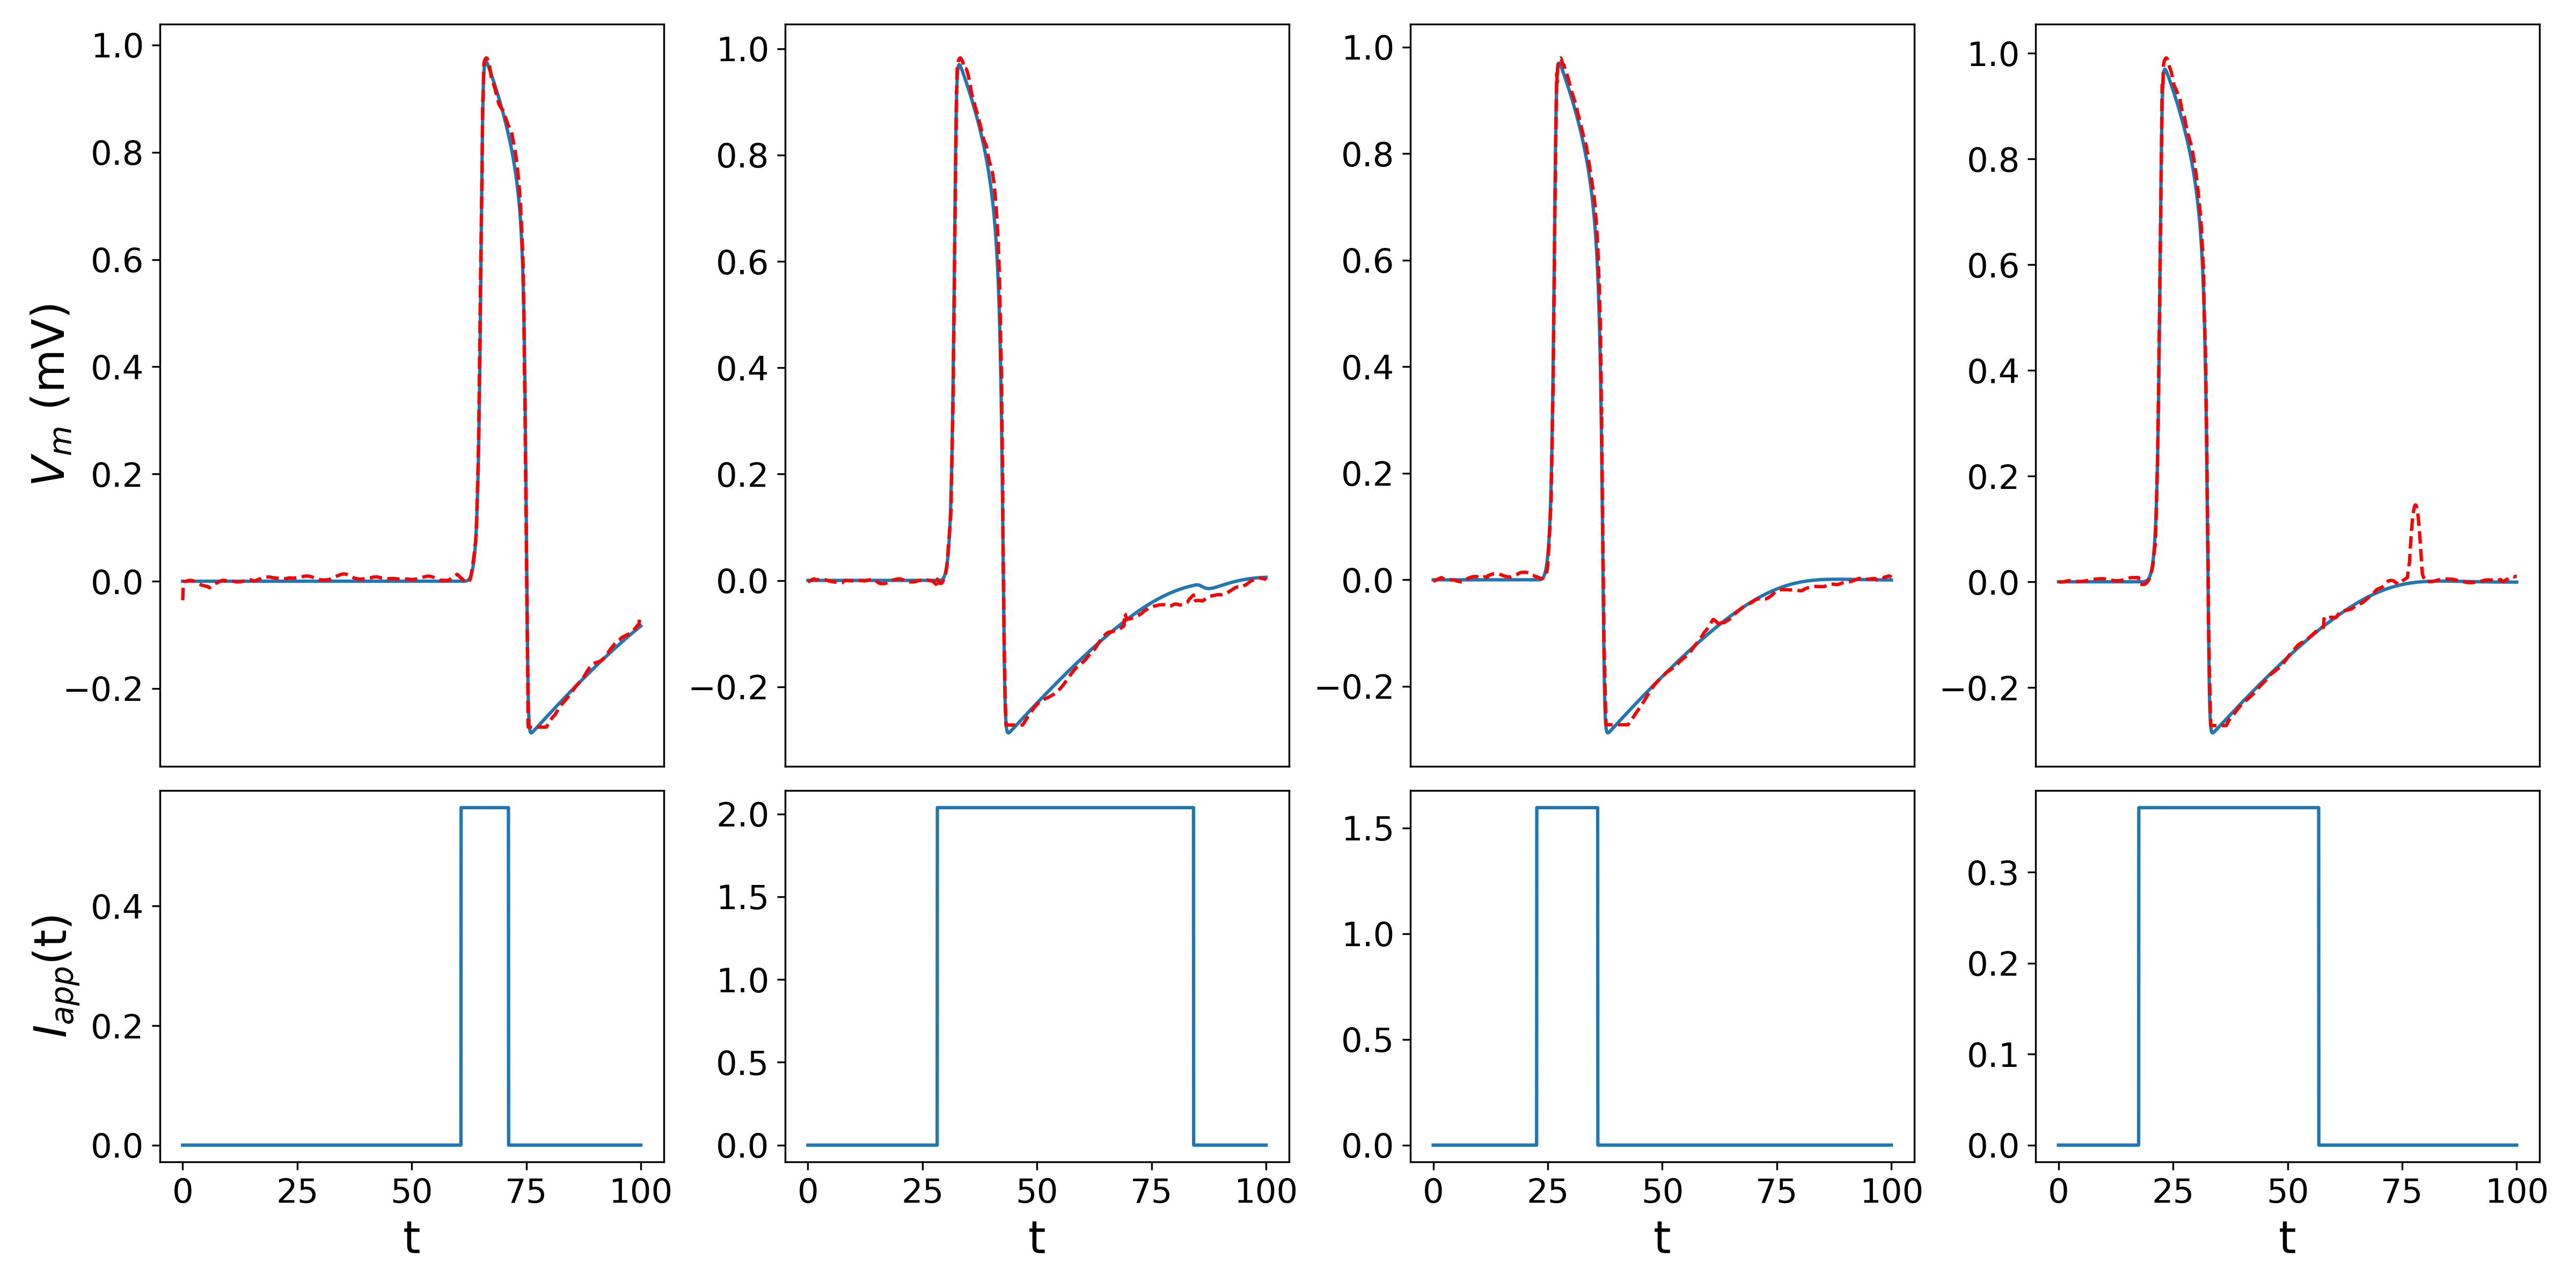
\includegraphics[width=\textwidth]{img/FH_model/ER_Network/FNO/HHpeaks_N=10.png}
        \caption{$N=10$}
    \end{subfigure}
    \hfill
    \begin{subfigure}[b]{0.32\textwidth}
        \centering
        
\includegraphics[width=\textwidth]{img/FH_model/ER_Network/FNO/HHpeaks_N=100.png}
        \caption{$N=100$}
    \end{subfigure}
    \hfill
    \begin{subfigure}[b]{0.32\textwidth}
        \centering
        
\includegraphics[width=\textwidth]{img/FH_model/ER_Network/FNO/HHpeaks_N=200.png}
        \caption{$N=200$}
    \end{subfigure}
    
    \vspace{0.4cm} % Spazio verticale tra le righe
    
    % --- Seconda riga ---
    \begin{subfigure}[b]{0.32\textwidth}
        \centering
        
\includegraphics[width=\textwidth]{img/FH_model/ER_Network/FNO/HHpeaks_N=300.png}
        \caption{$N=300$}
    \end{subfigure}
    \hfill
    \begin{subfigure}[b]{0.32\textwidth}
        \centering
        
\includegraphics[width=\textwidth]{img/FH_model/ER_Network/FNO/HHpeaks_N=400.png}
        \caption{$N=400$}
    \end{subfigure}
    \hfill
    \begin{subfigure}[b]{0.32\textwidth}
        \centering
        
\includegraphics[width=\textwidth]{img/FH_model/ER_Network/FNO/HHpeaks_N=500.png}
        \caption{$N=500$}
    \end{subfigure}
    
    \vspace{0.4cm}
    
    % --- Terza riga ---
    \begin{subfigure}[b]{0.32\textwidth}
        \centering
        
\includegraphics[width=\textwidth]{img/FH_model/ER_Network/FNO/HHpeaks_N=600.png}
        \caption{$N=600$}
    \end{subfigure}
    \hfill
    \begin{subfigure}[b]{0.32\textwidth}
        \centering
        
\includegraphics[width=\textwidth]{img/FH_model/ER_Network/FNO/HHpeaks_N=700.png}
        \caption{$N=700$}
    \end{subfigure}
    \hfill
    \begin{subfigure}[b]{0.32\textwidth}
        \centering
        
\includegraphics[width=\textwidth]{img/FH_model/ER_Network/FNO/HHpeaks_N=800.png}
        \caption{$N=800$}
    \end{subfigure}
    
    \vspace{0.4cm}
    
    % --- Quarta riga ---
    \begin{subfigure}[b]{0.32\textwidth}
        \centering
        
\includegraphics[width=\textwidth]{img/FH_model/ER_Network/FNO/HHpeaks_N=900.png}
        \caption{$N=900$}
    \end{subfigure}
    \hfill
    \begin{subfigure}[b]{0.32\textwidth}
        \centering
        
\includegraphics[width=\textwidth]{img/FH_model/ER_Network/FNO/HHpeaks_N=1000.png}
        \caption{$N=1000$}
    \end{subfigure}
    \hfill
    \begin{subfigure}[b]{0.32\textwidth}
        \centering
        
\includegraphics[width=\textwidth]{img/FH_model/ER_Network/FNO/HHpeaks_N=2000.png}
        \caption{$N=2000$}
    \end{subfigure}
    
    \caption{Some instances of the test set for different Erd\H{o}s-R\'enyi network sizes ($N$).  For each column we can see the applied input current (bottom) with its corresponding potential response (top): the blue line represents the result of the simulations, whereas the dotted red line indicates the output of the NN.}
    \label{fig:er_peaks_grid}
\end{figure}


%%%
% ==========================================
% GRIGLIA 1: MSE HISTOGRAMS

%Devo rifarli ? alcune cifre sull'asse x si sovrappongono e forse dovrei usare la notazione scientifica per Mean=. ???
% ==========================================

\begin{figure}[htbp]
    \centering
    % --- Prima riga ---
    \begin{subfigure}[b]{0.32\textwidth}
        \centering
        
\includegraphics[width=\textwidth]{img/FH_model/ER_Network/FNO/L2histoFNO_N=10.png}
        \caption{$N=10$}
    \end{subfigure}
    \hfill
    \begin{subfigure}[b]{0.32\textwidth}
        \centering
        
\includegraphics[width=\textwidth]{img/FH_model/ER_Network/FNO/L2histoFNO_N=100.png}
        \caption{$N=100$}
    \end{subfigure}
    \hfill
    \begin{subfigure}[b]{0.32\textwidth}
        \centering
        
\includegraphics[width=\textwidth]{img/FH_model/ER_Network/FNO/L2histoFNO_N=200.png}
        \caption{$N=200$}
    \end{subfigure}
    
    \vspace{0.4cm}
    
    % --- Seconda riga ---
    \begin{subfigure}[b]{0.32\textwidth}
        \centering
        
\includegraphics[width=\textwidth]{img/FH_model/ER_Network/FNO/L2histoFNO_N=300.png}
        \caption{$N=300$}
    \end{subfigure}
    \hfill
    \begin{subfigure}[b]{0.32\textwidth}
        \centering
        
\includegraphics[width=\textwidth]{img/FH_model/ER_Network/FNO/L2histoFNO_N=400.png}
        \caption{$N=400$}
    \end{subfigure}
    \hfill
    \begin{subfigure}[b]{0.32\textwidth}
        \centering
        
\includegraphics[width=\textwidth]{img/FH_model/ER_Network/FNO/L2histoFNO_N=500.png}
        \caption{$N=500$}
    \end{subfigure}
    
    \vspace{0.4cm}
    
    % --- Terza riga ---
    \begin{subfigure}[b]{0.32\textwidth}
        \centering
        
\includegraphics[width=\textwidth]{img/FH_model/ER_Network/FNO/L2histoFNO_N=600.png}
        \caption{$N=600$}
    \end{subfigure}
    \hfill
    \begin{subfigure}[b]{0.32\textwidth}
        \centering
        
\includegraphics[width=\textwidth]{img/FH_model/ER_Network/FNO/L2histoFNO_N=700.png}
        \caption{$N=700$}
    \end{subfigure}
    \hfill
    \begin{subfigure}[b]{0.32\textwidth}
        \centering
        
\includegraphics[width=\textwidth]{img/FH_model/ER_Network/FNO/L2histoFNO_N=800.png}
        \caption{$N=800$}
    \end{subfigure}
    
    \vspace{0.4cm}
    
    % --- Quarta riga ---
    \begin{subfigure}[b]{0.32\textwidth}
        \centering
        
\includegraphics[width=\textwidth]{img/FH_model/ER_Network/FNO/L2histoFNO_N=900.png}
        \caption{$N=900$}
    \end{subfigure}
    \hfill
    \begin{subfigure}[b]{0.32\textwidth}
        \centering
        
\includegraphics[width=\textwidth]{img/FH_model/ER_Network/FNO/L2histoFNO_N=1000.png}
        \caption{$N=1000$}
    \end{subfigure}
    \hfill
    \begin{subfigure}[b]{0.32\textwidth}
        \centering
        
\includegraphics[width=\textwidth]{img/FH_model/ER_Network/FNO/L2histoFNO_N=2000.png}
        \caption{$N=2000$}
    \end{subfigure}
    
    \caption{MSE error distributions across the test set for different Erd\H{o}s-R\'enyi network sizes ($N$).}
    \label{fig:er_histo_grid}
\end{figure}

% ==========================================
% GRIGLIA 2: LOSS PLOTS
% ==========================================
\begin{figure}[htbp]
    \centering
    % --- Prima riga ---
    \begin{subfigure}[b]{0.32\textwidth}
        \centering
        
\includegraphics[width=\textwidth]{img/FH_model/ER_Network/FNO/loss_plot_fixed_N=10.png}
        \caption{$N=10$}
    \end{subfigure}
    \hfill
    \begin{subfigure}[b]{0.32\textwidth}
        \centering
        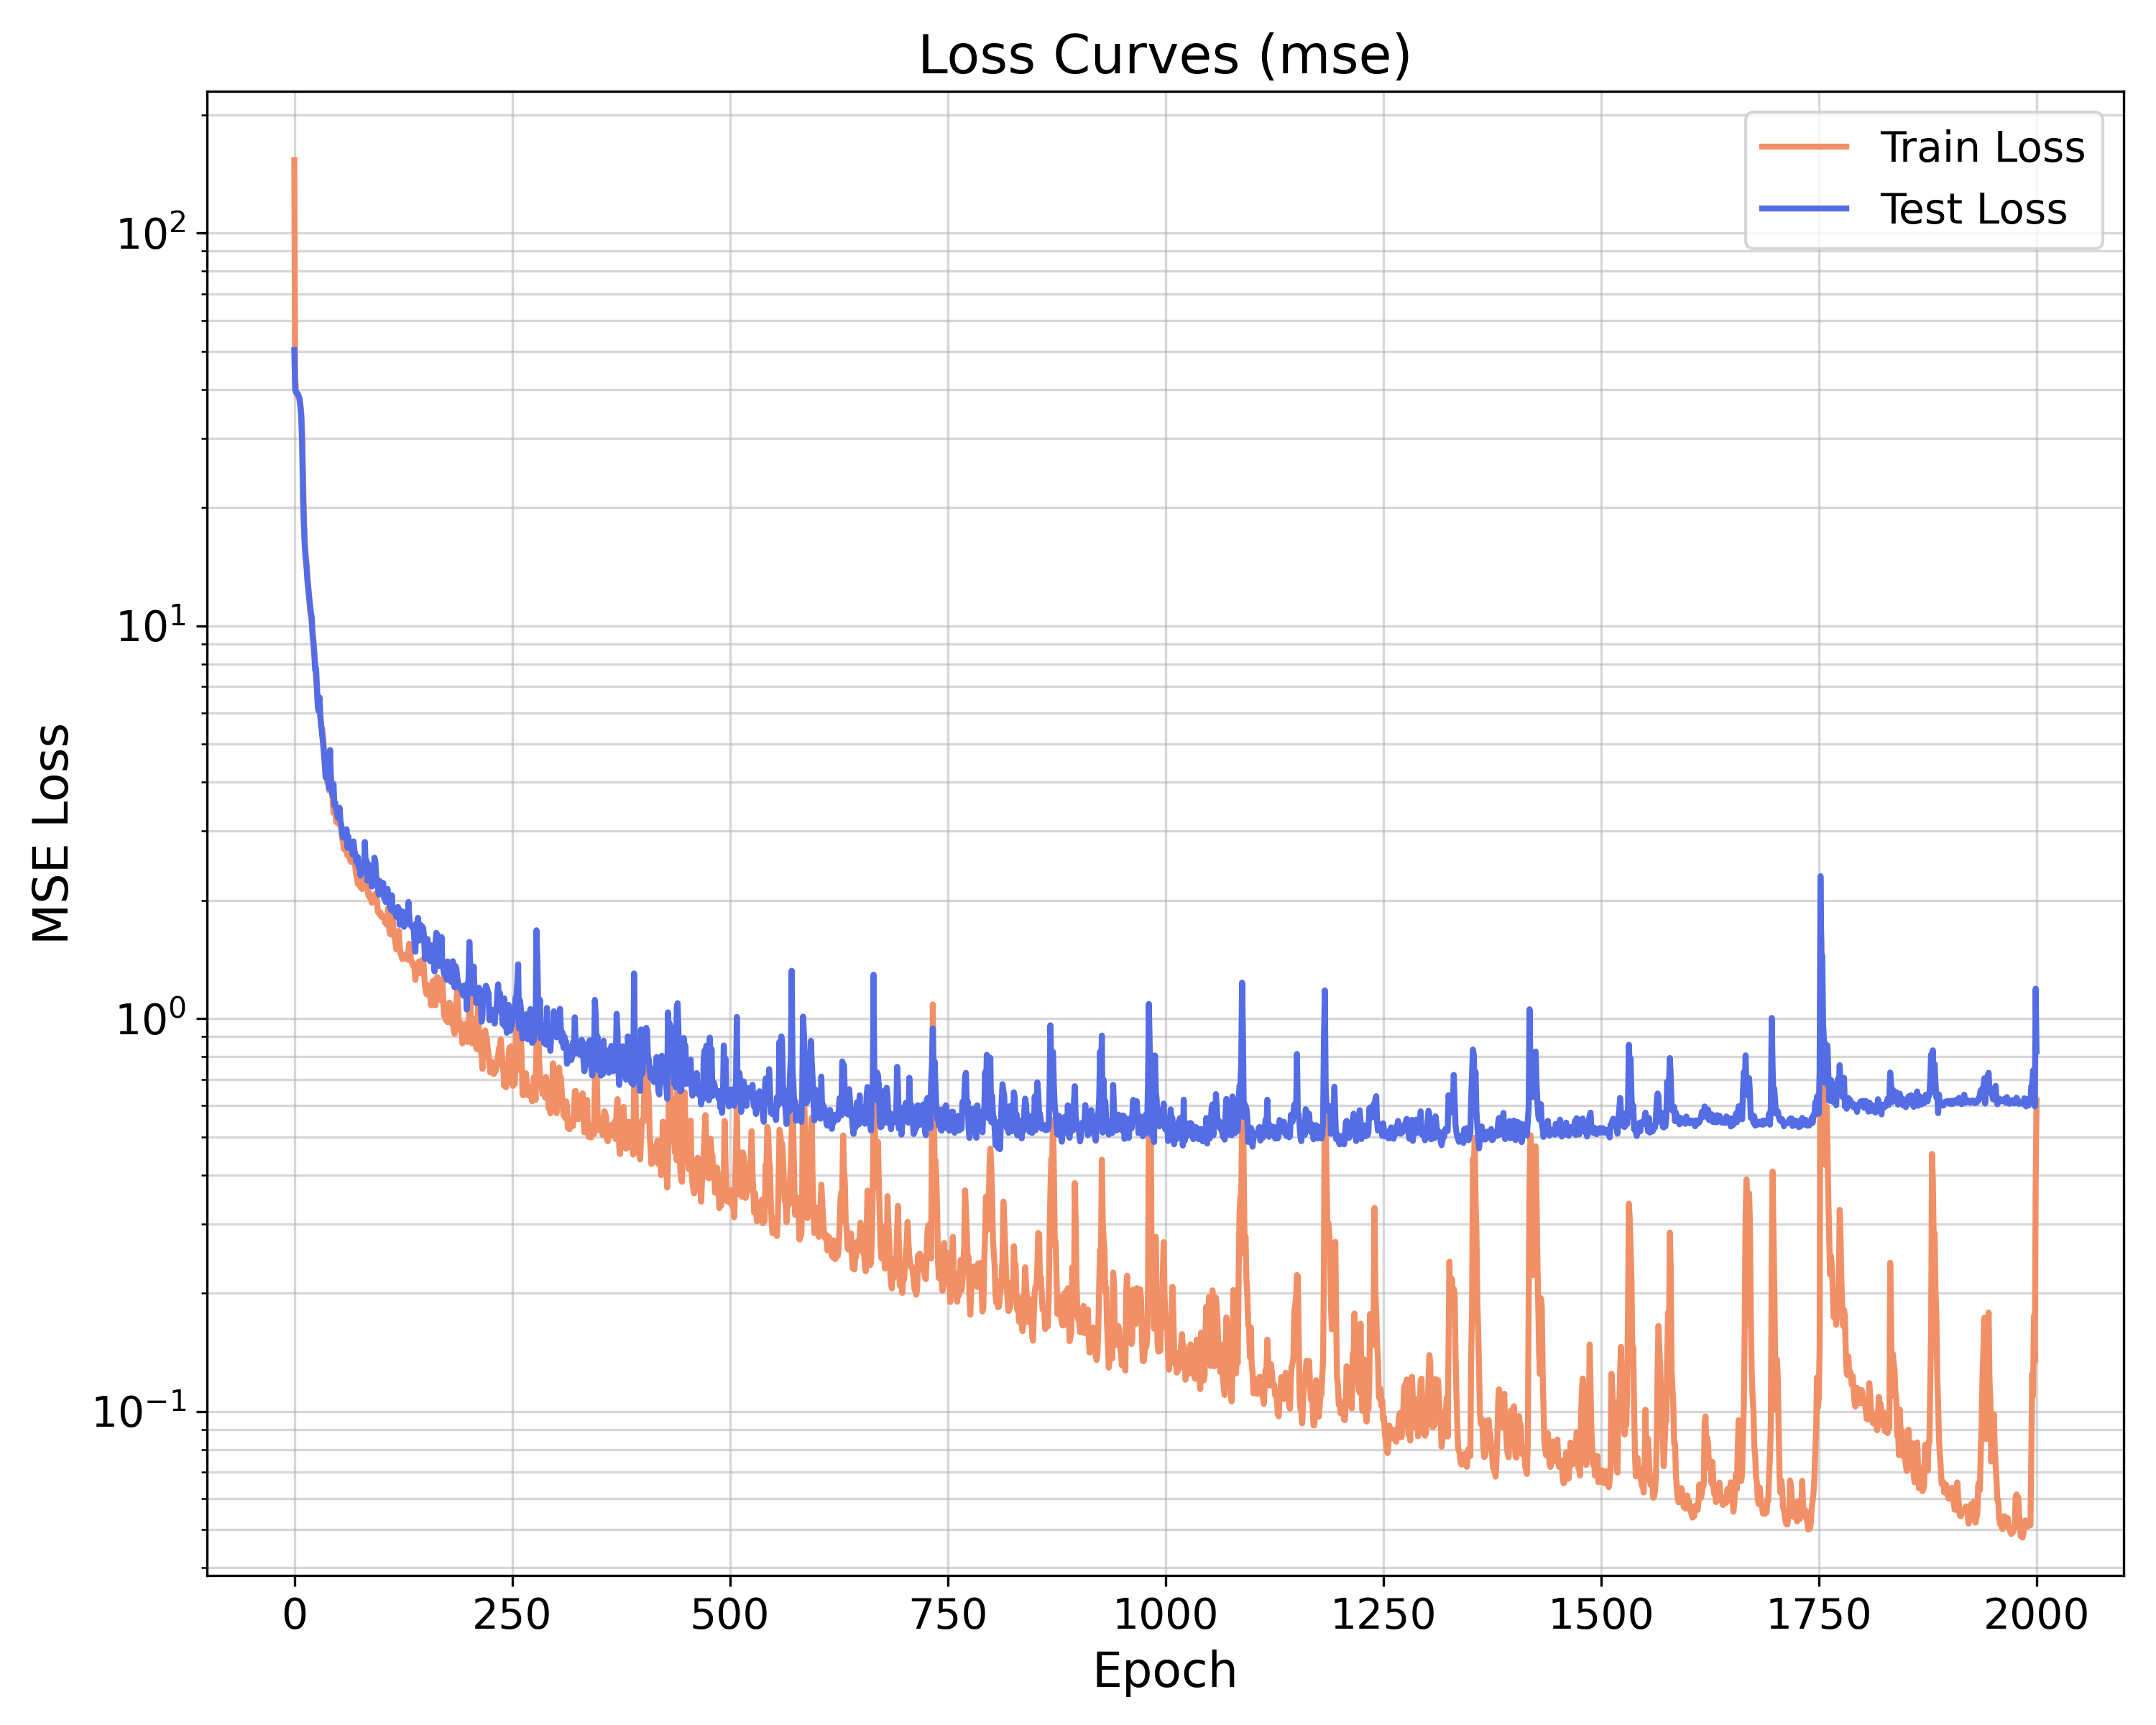
\includegraphics[width=\textwidth]{img/FH_model/ER_Network/FNO/loss_plot_fixed_N=100.png}
        \caption{$N=100$}
    \end{subfigure}
    \hfill
    \begin{subfigure}[b]{0.32\textwidth}
        \centering
        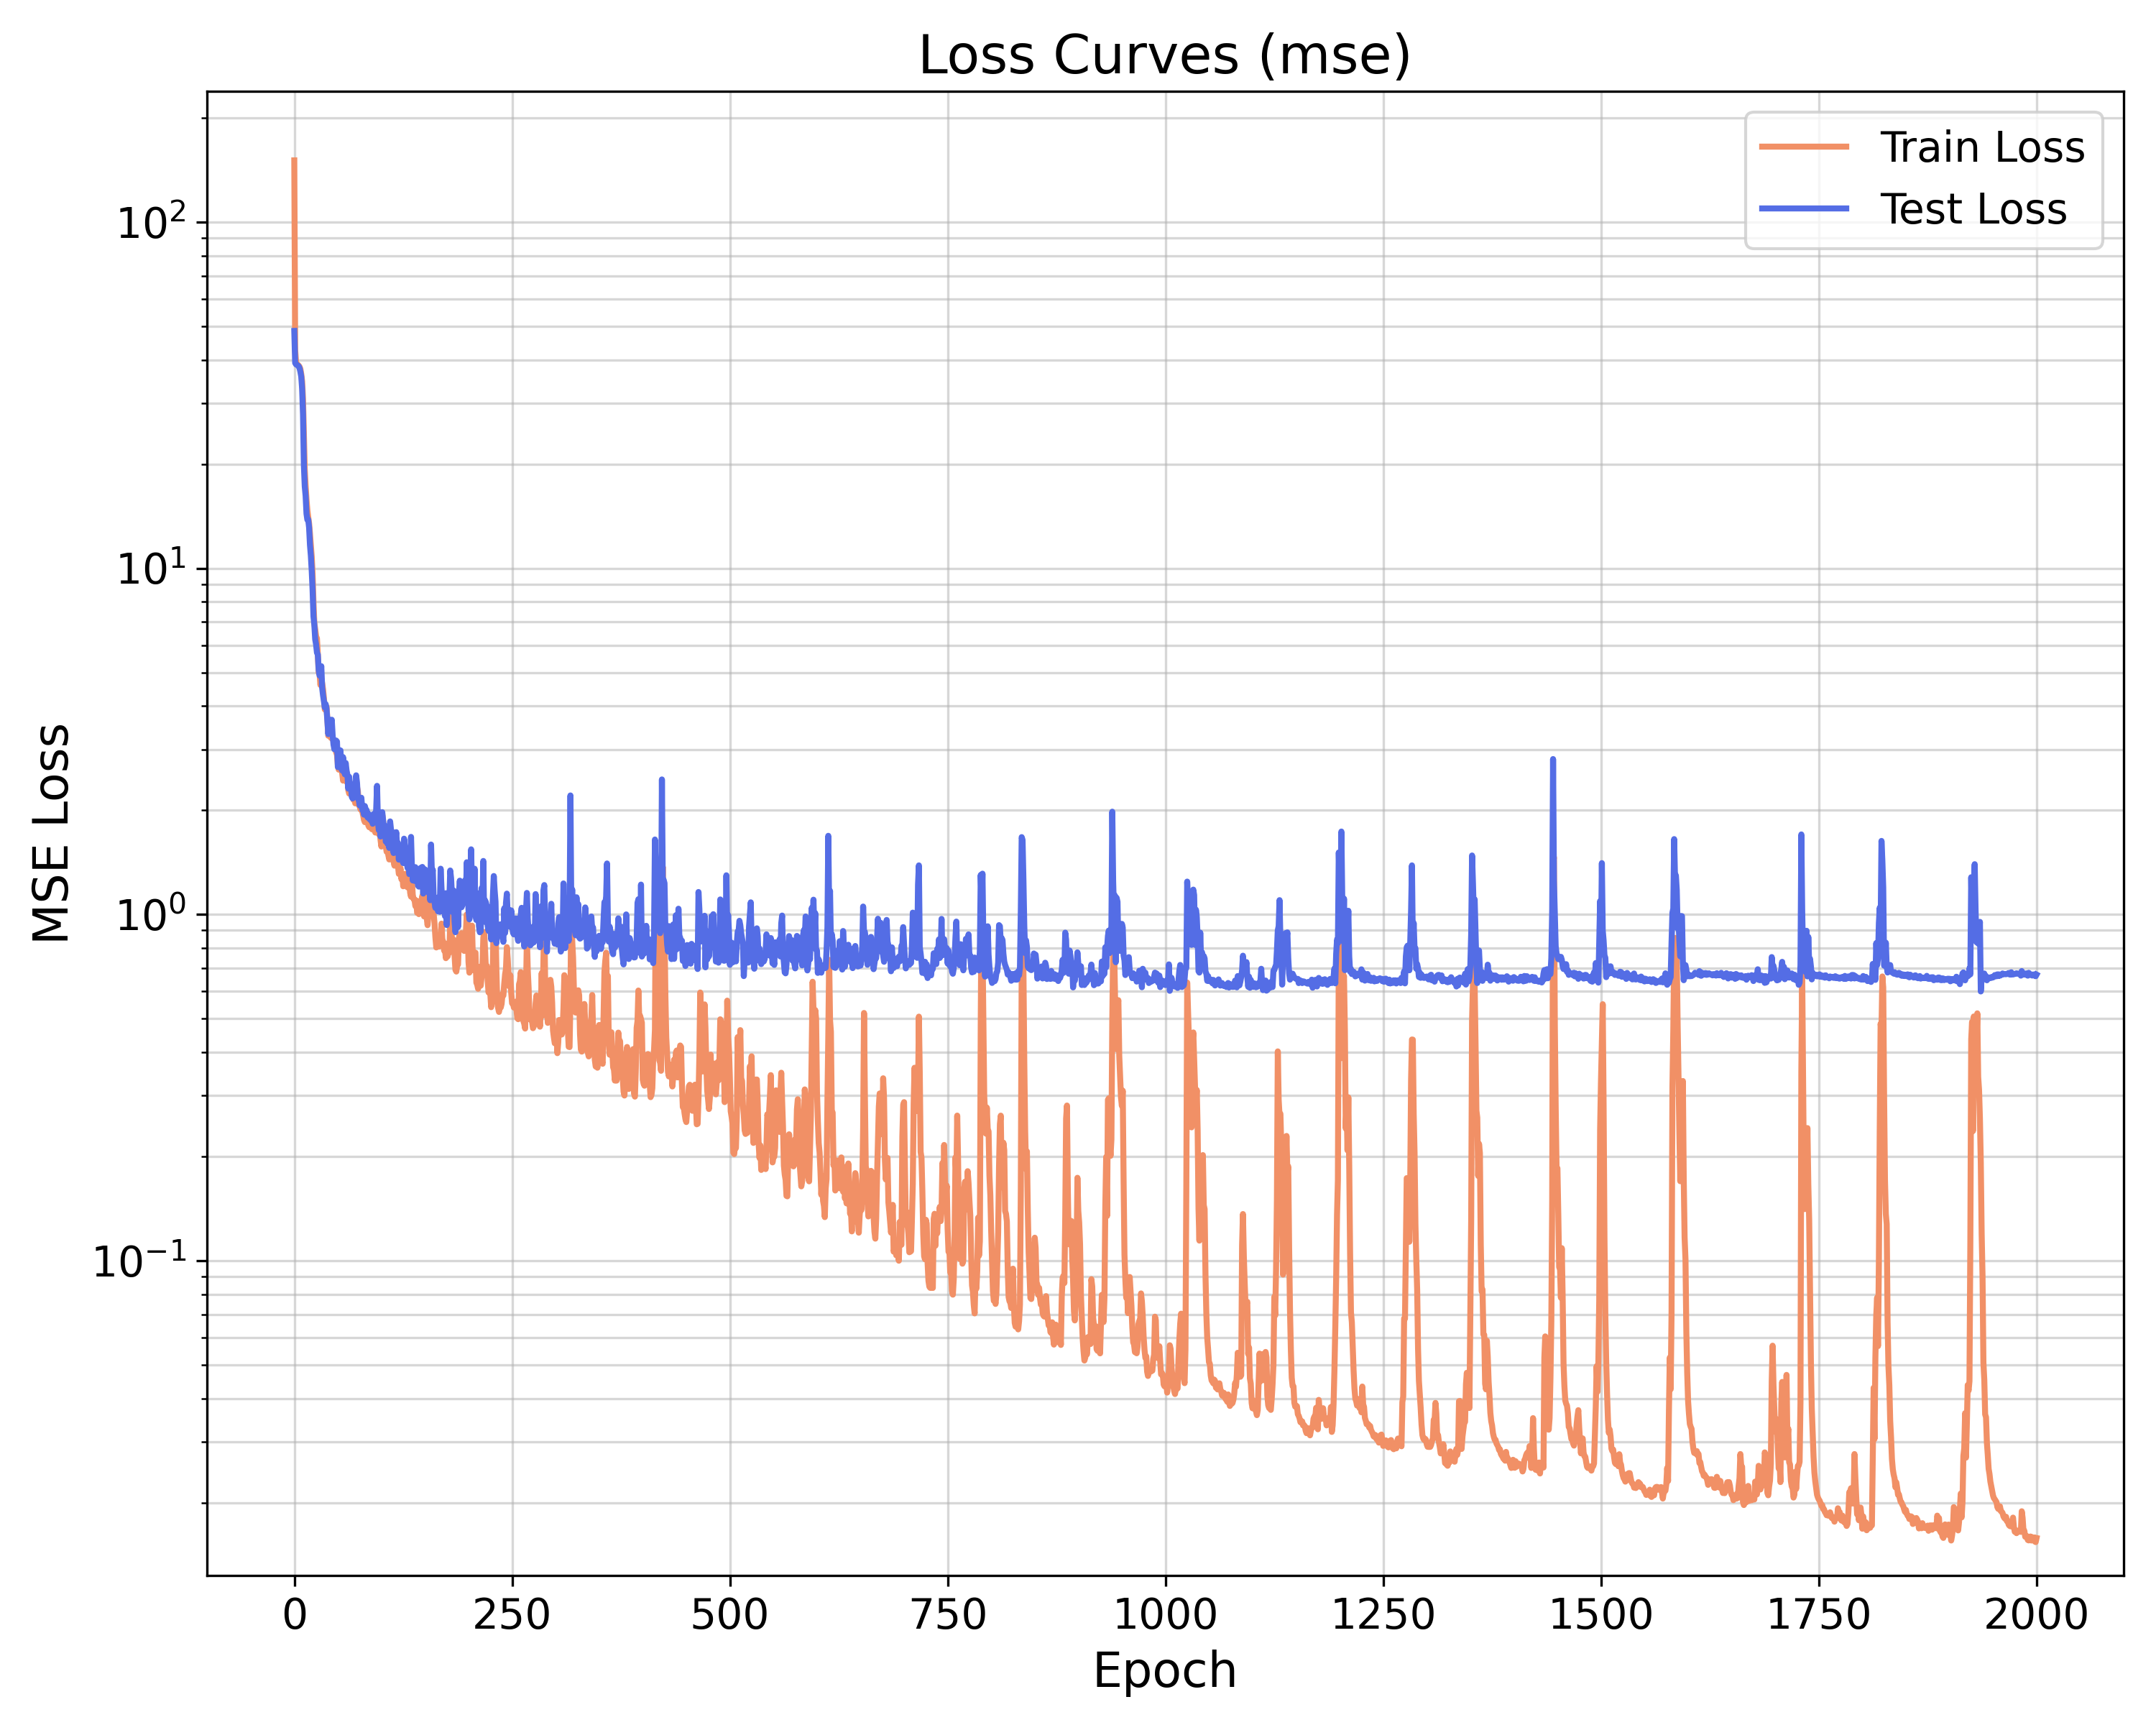
\includegraphics[width=\textwidth]{img/FH_model/ER_Network/FNO/loss_plot_fixed_N=200.png}
        \caption{$N=200$}
    \end{subfigure}
    
    \vspace{0.4cm}
    
    % --- Seconda riga ---
    \begin{subfigure}[b]{0.32\textwidth}
        \centering
        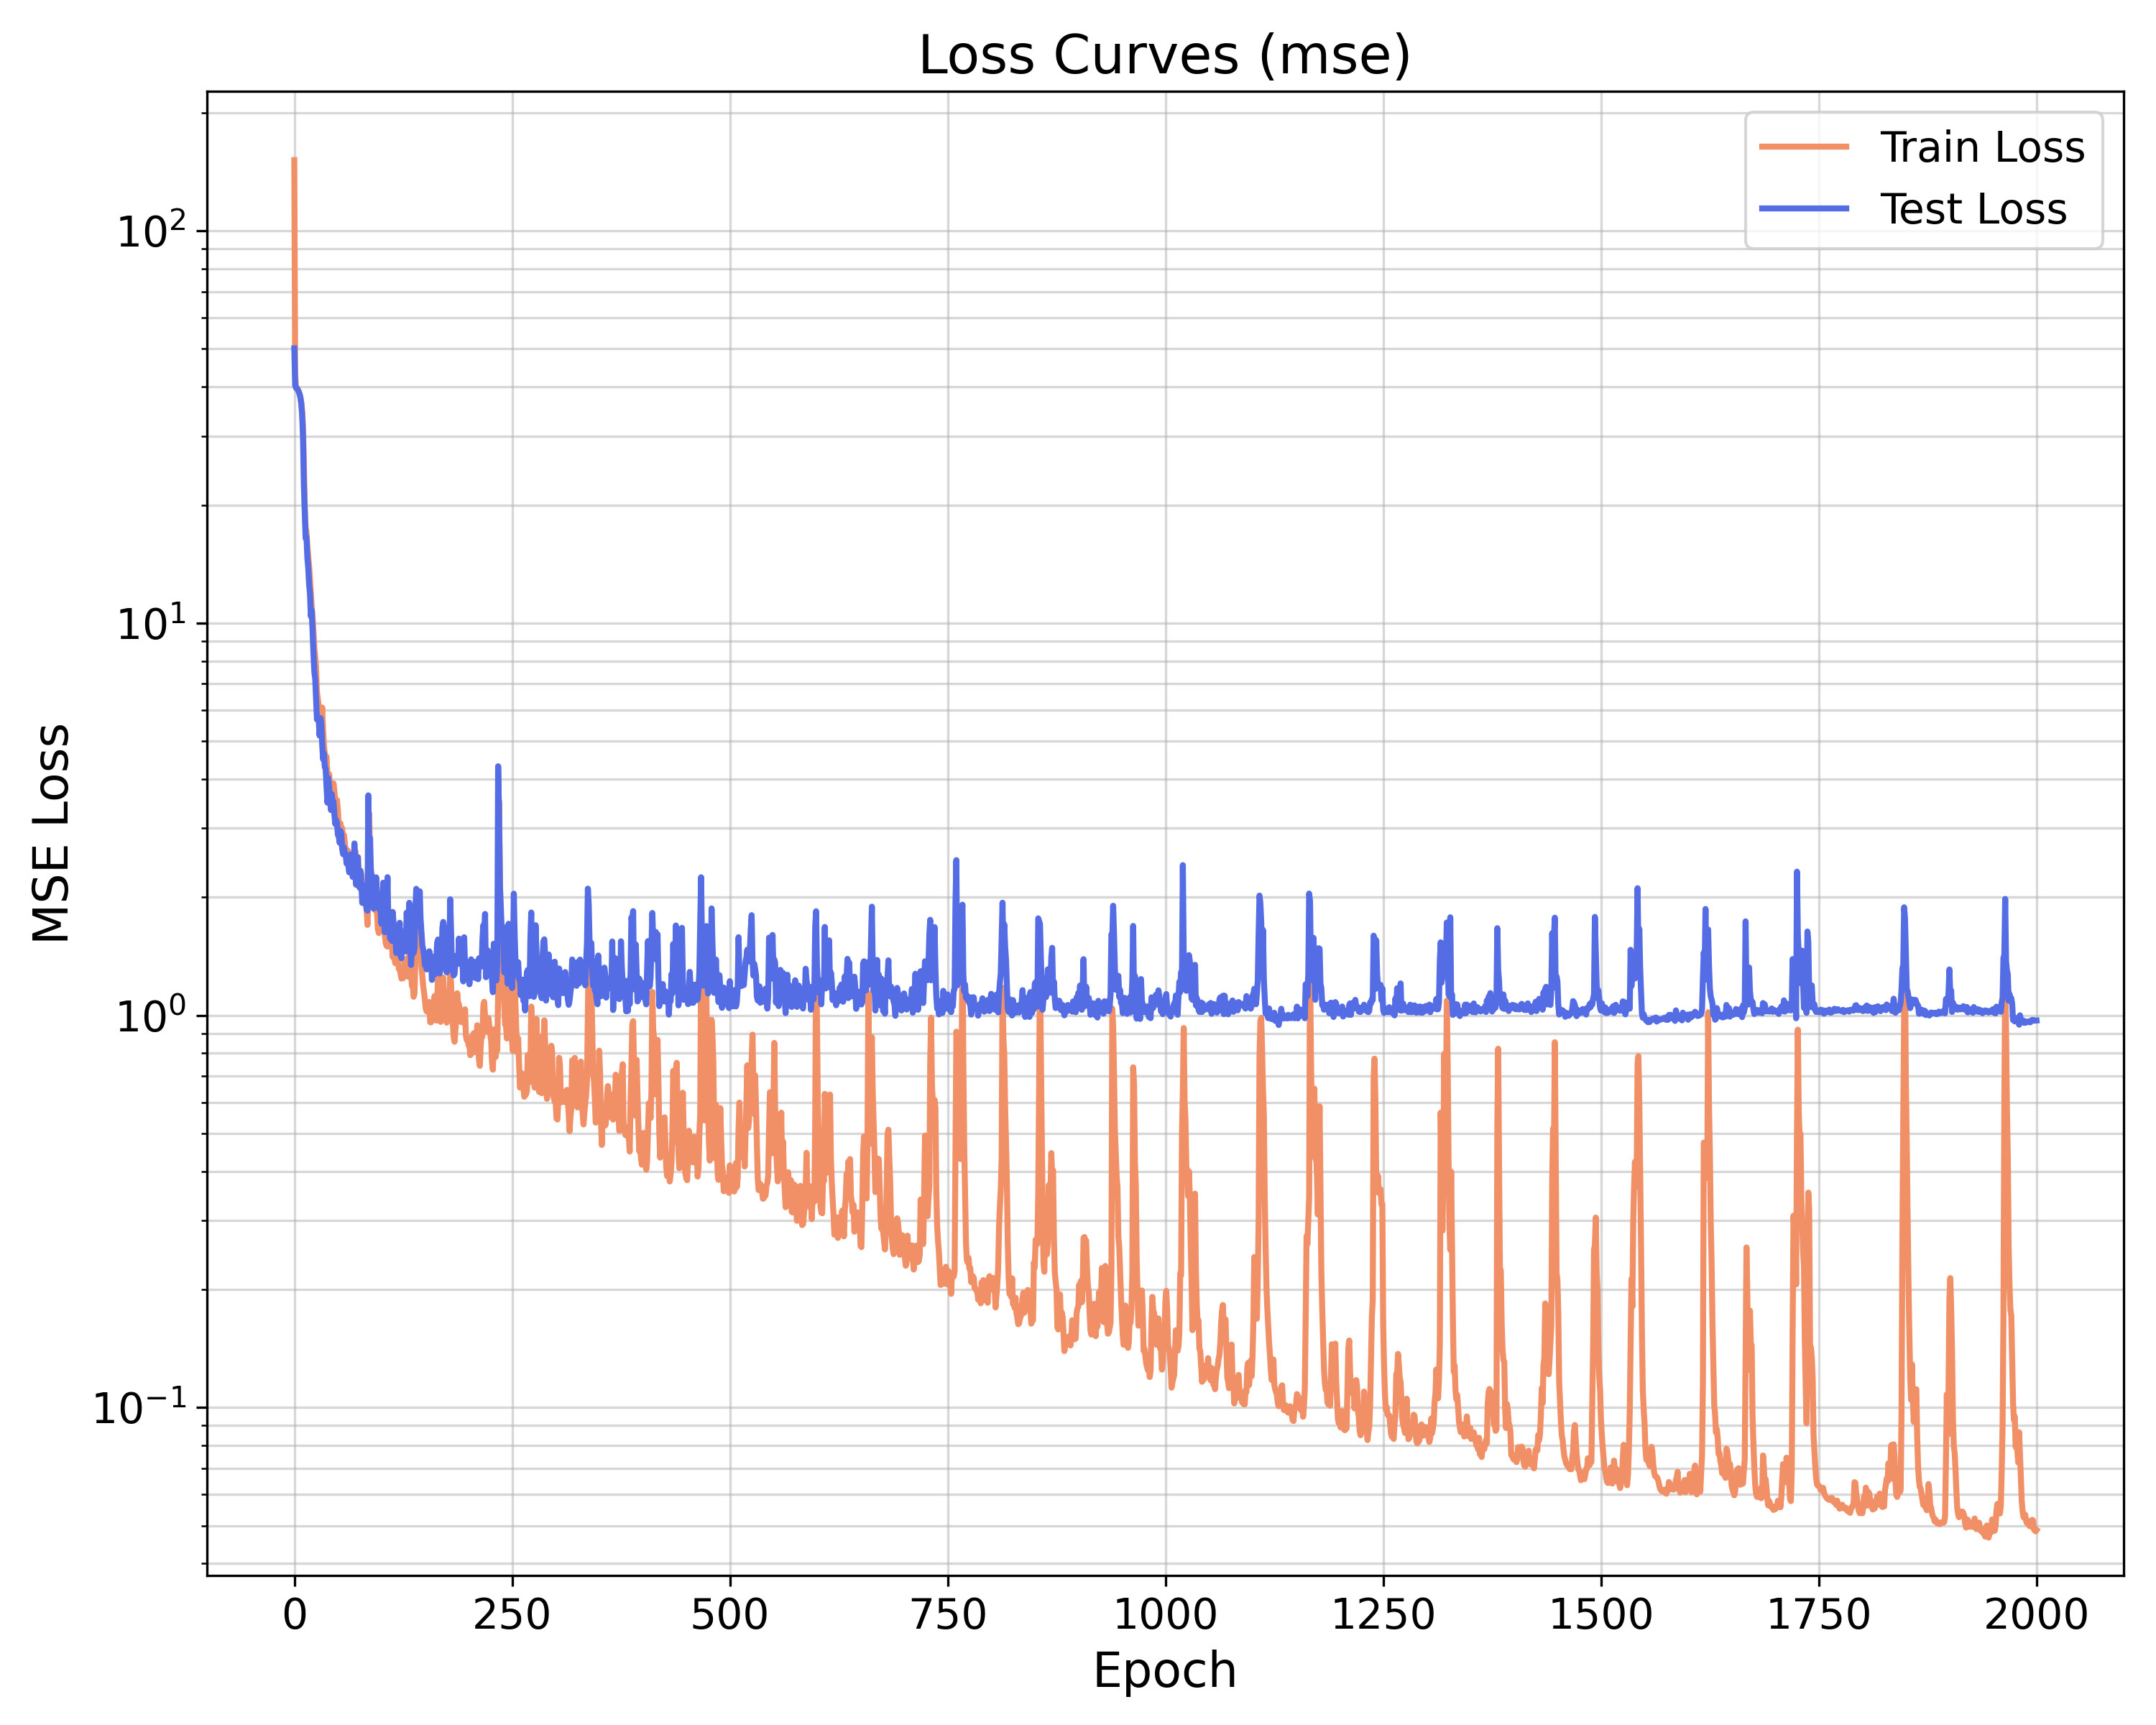
\includegraphics[width=\textwidth]{img/FH_model/ER_Network/FNO/loss_plot_fixed_N=300.png}
        \caption{$N=300$}
    \end{subfigure}
    \hfill
    \begin{subfigure}[b]{0.32\textwidth}
        \centering
        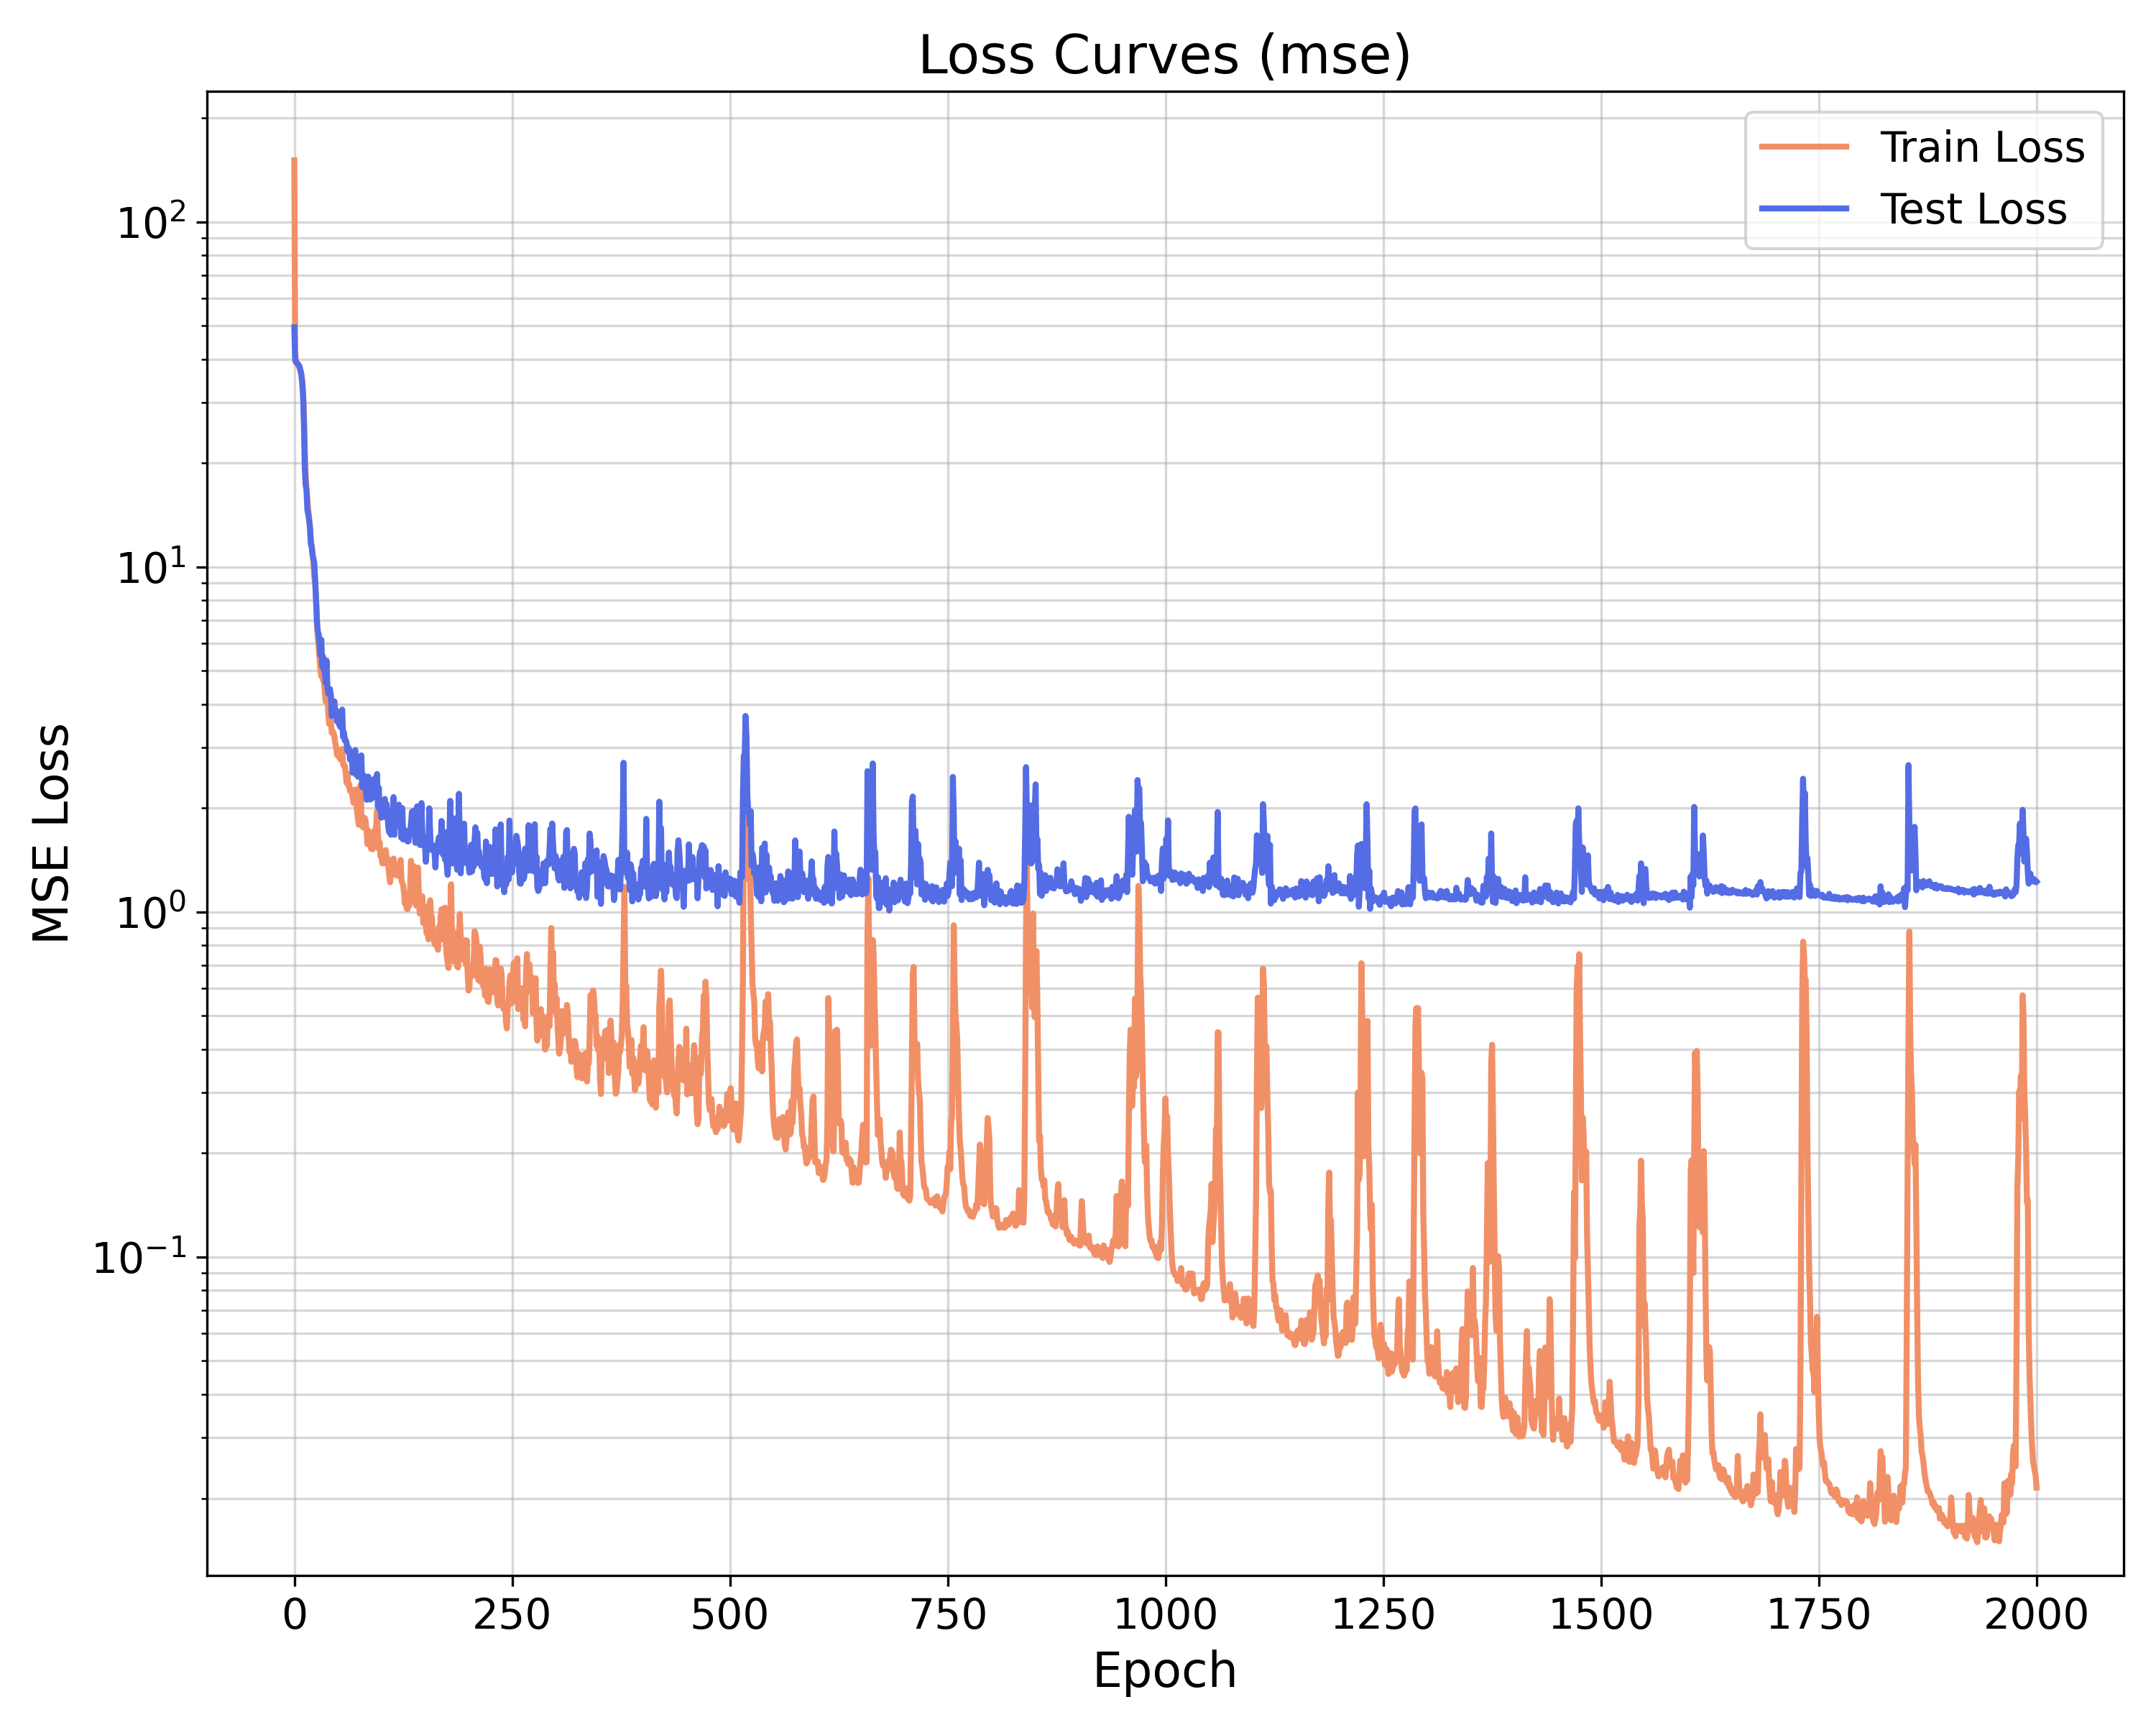
\includegraphics[width=\textwidth]{img/FH_model/ER_Network/FNO/loss_plot_fixed_N=400.png}
        \caption{$N=400$}
    \end{subfigure}
    \hfill
    \begin{subfigure}[b]{0.32\textwidth}
        \centering
        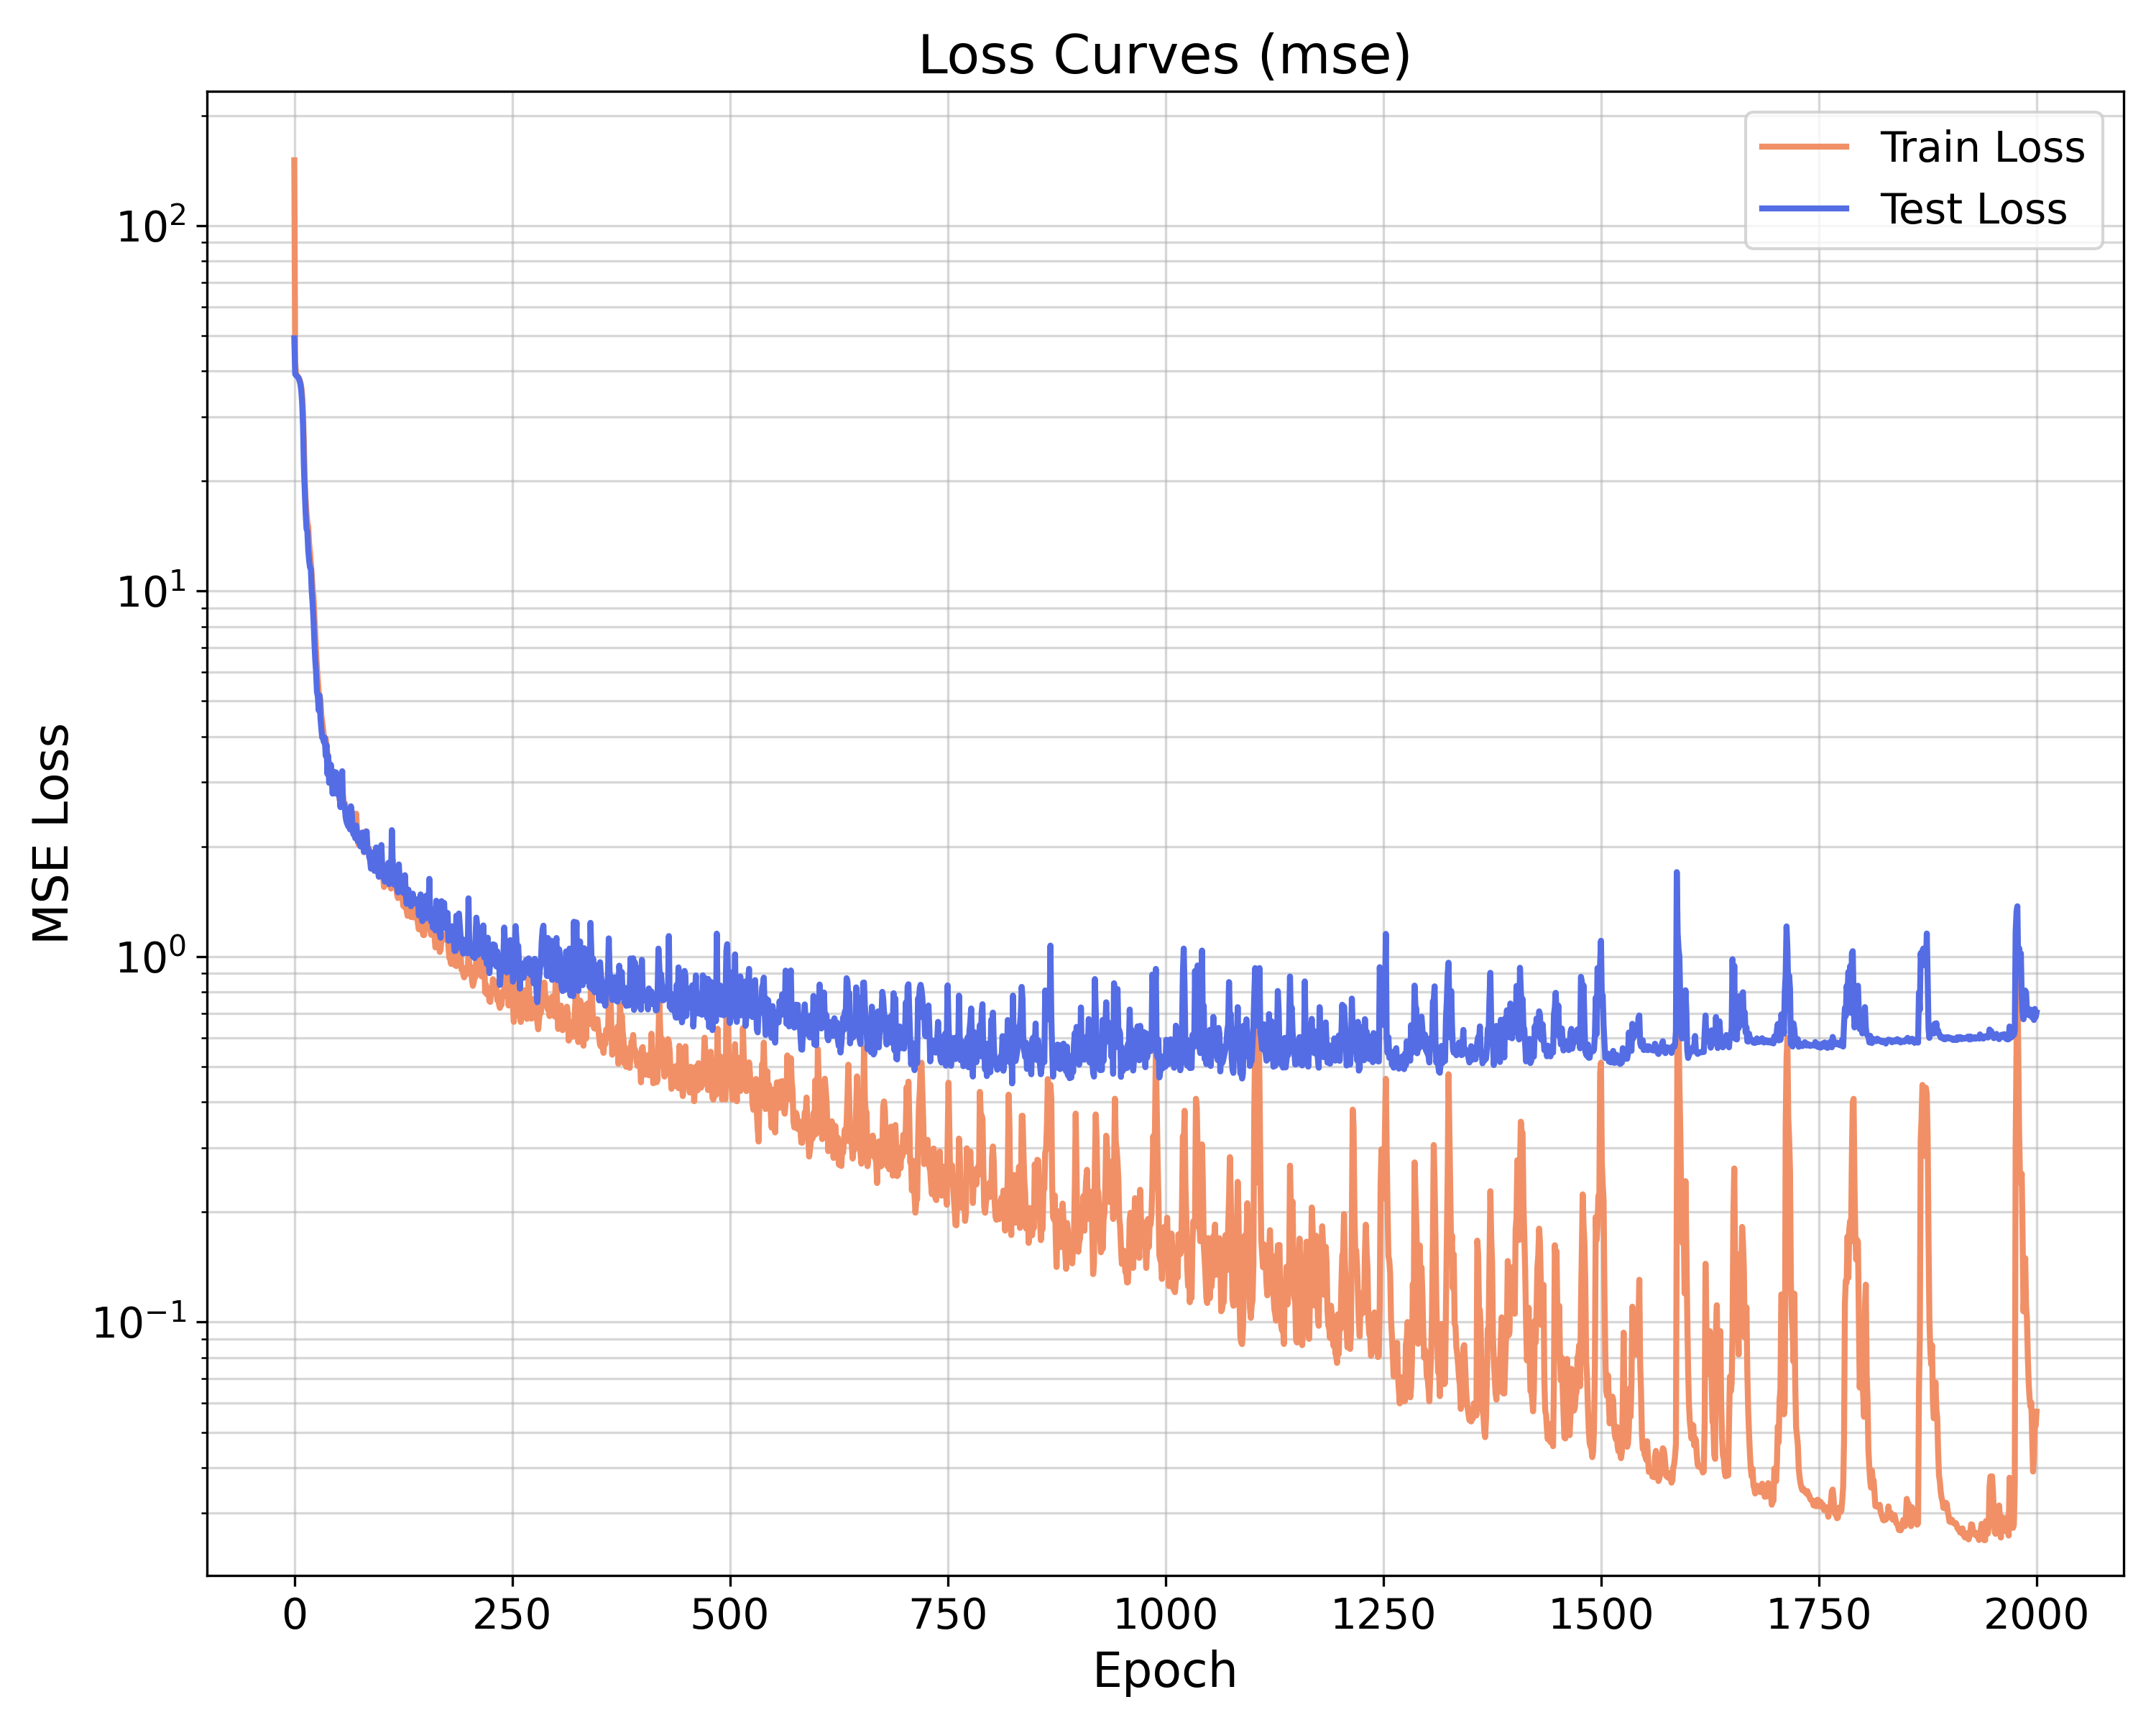
\includegraphics[width=\textwidth]{img/FH_model/ER_Network/FNO/loss_plot_fixed_N=500.png}
        \caption{$N=500$}
    \end{subfigure}
    
    \vspace{0.4cm}
    
    % --- Terza riga ---
    \begin{subfigure}[b]{0.32\textwidth}
        \centering
        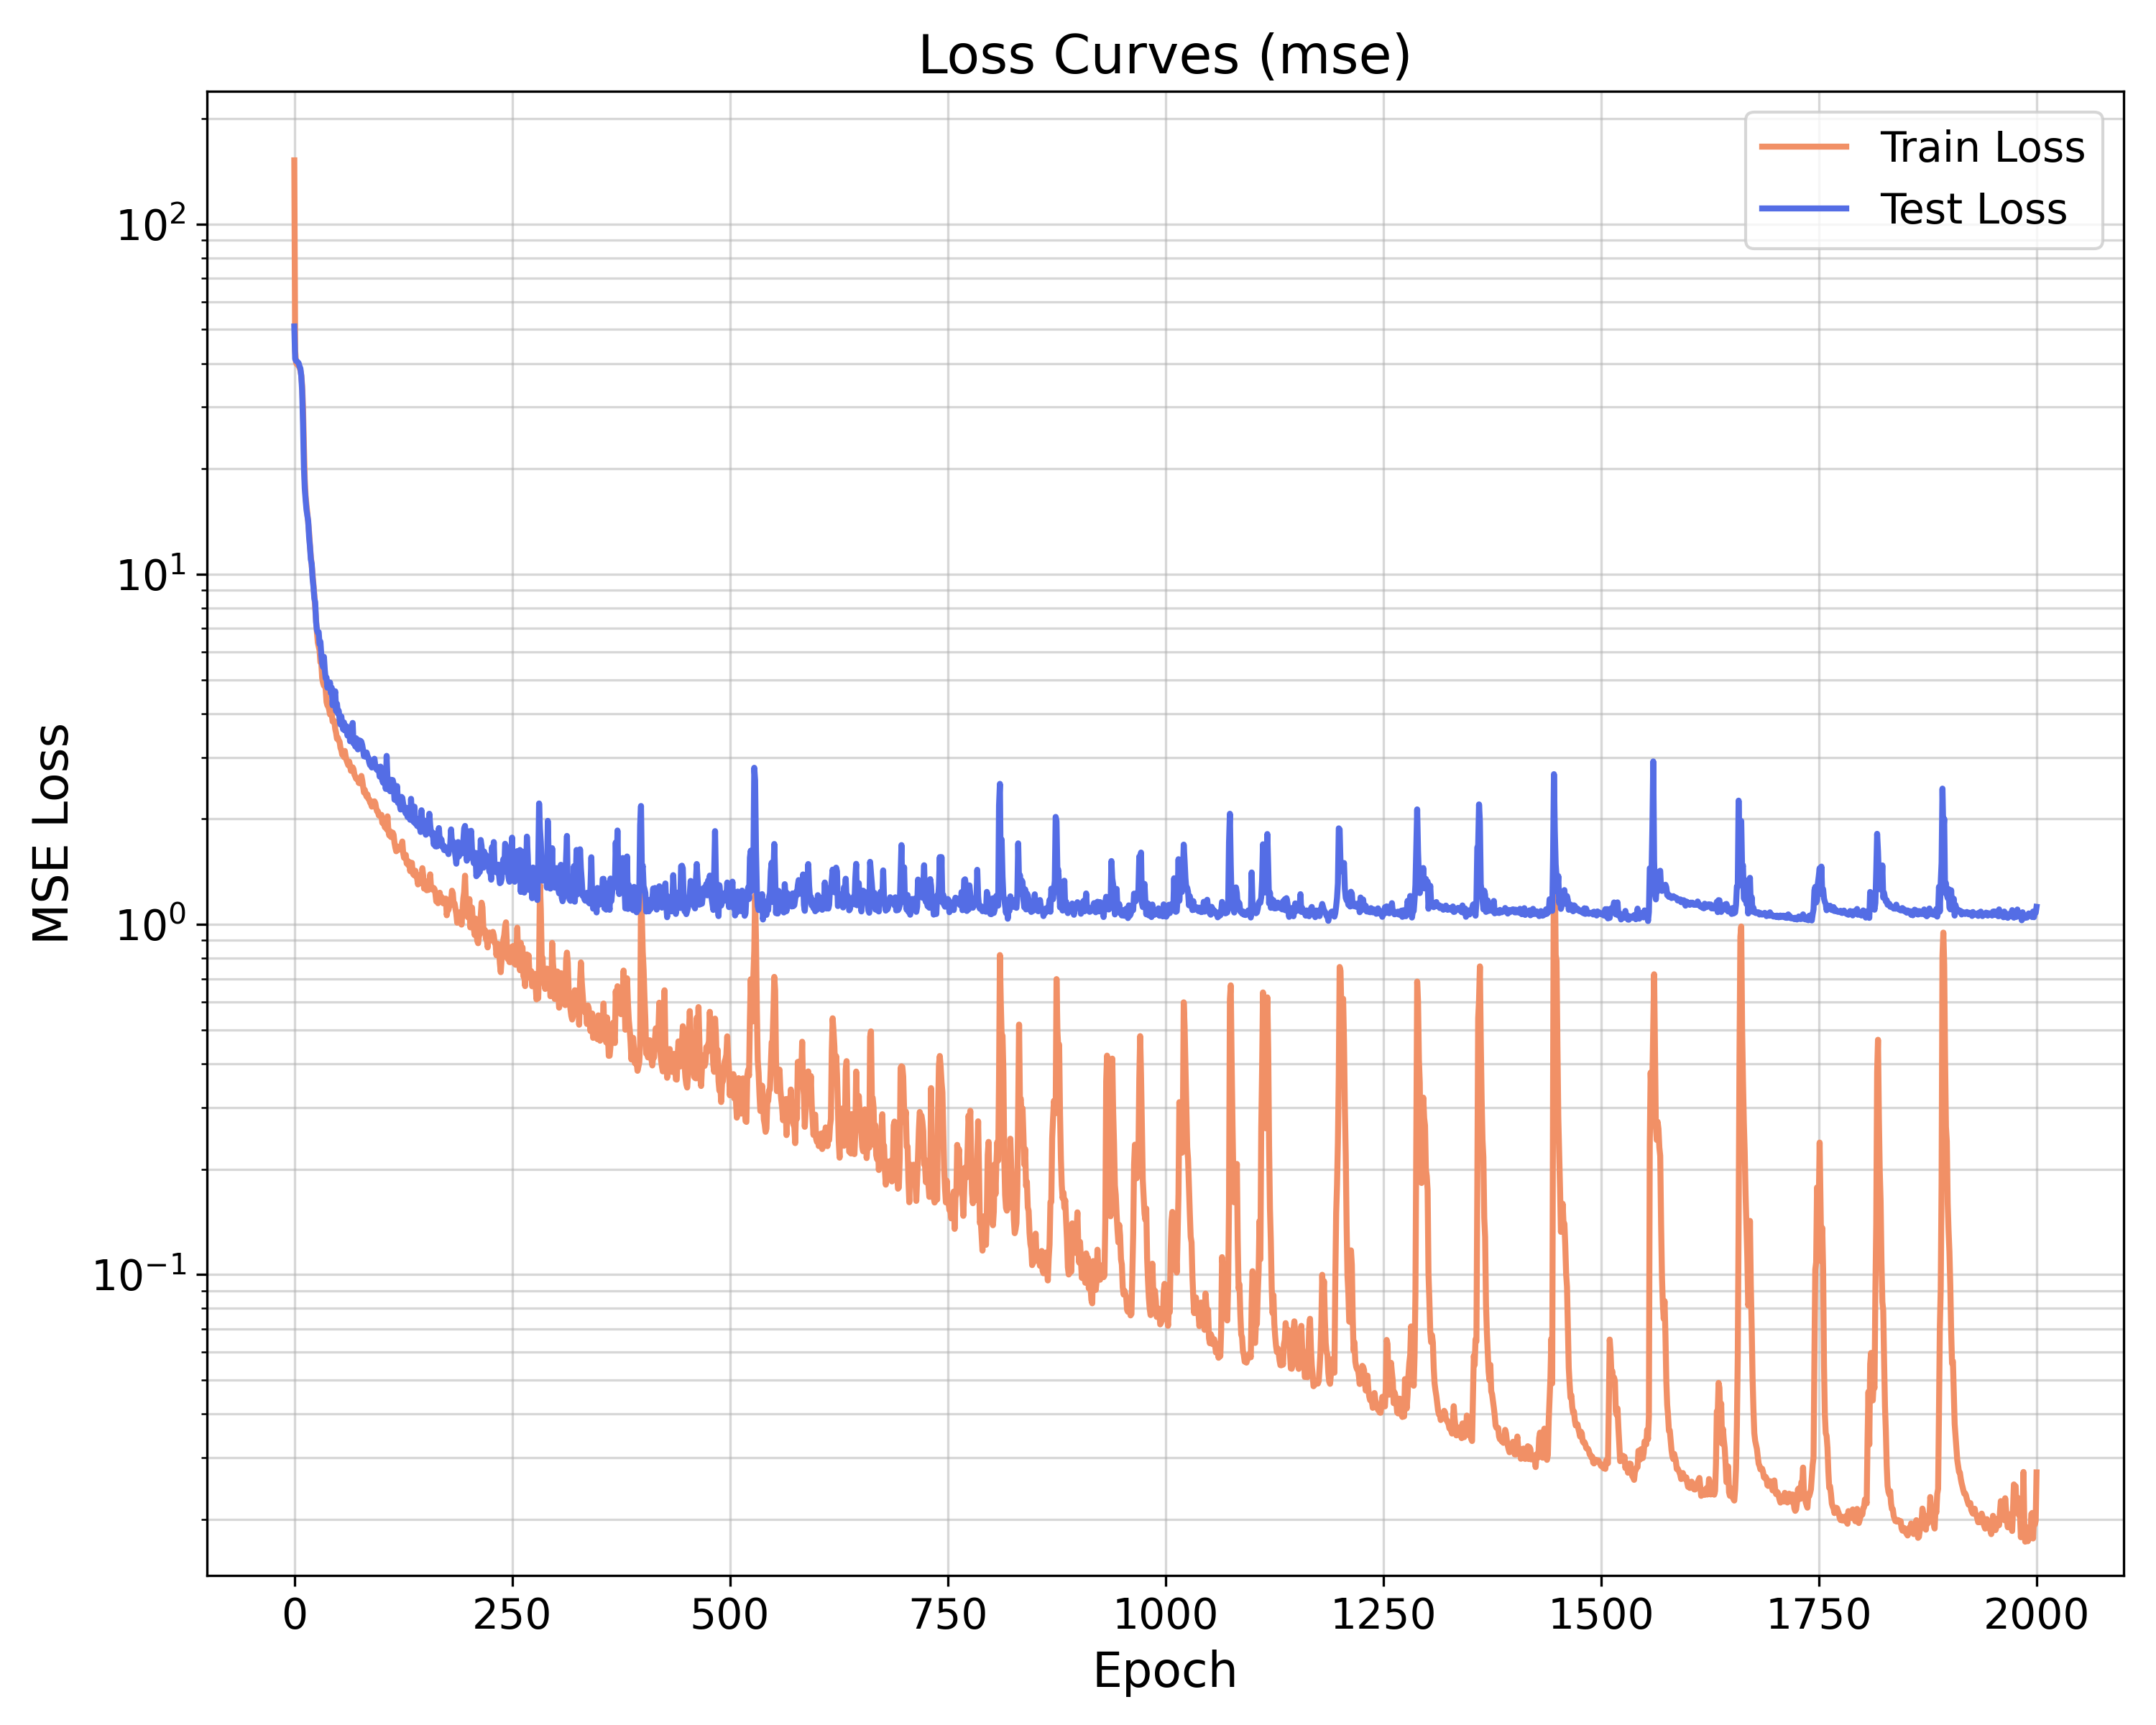
\includegraphics[width=\textwidth]{img/FH_model/ER_Network/FNO/loss_plot_fixed_N=600.png}
        \caption{$N=600$}
    \end{subfigure}
    \hfill
    \begin{subfigure}[b]{0.32\textwidth}
        \centering
        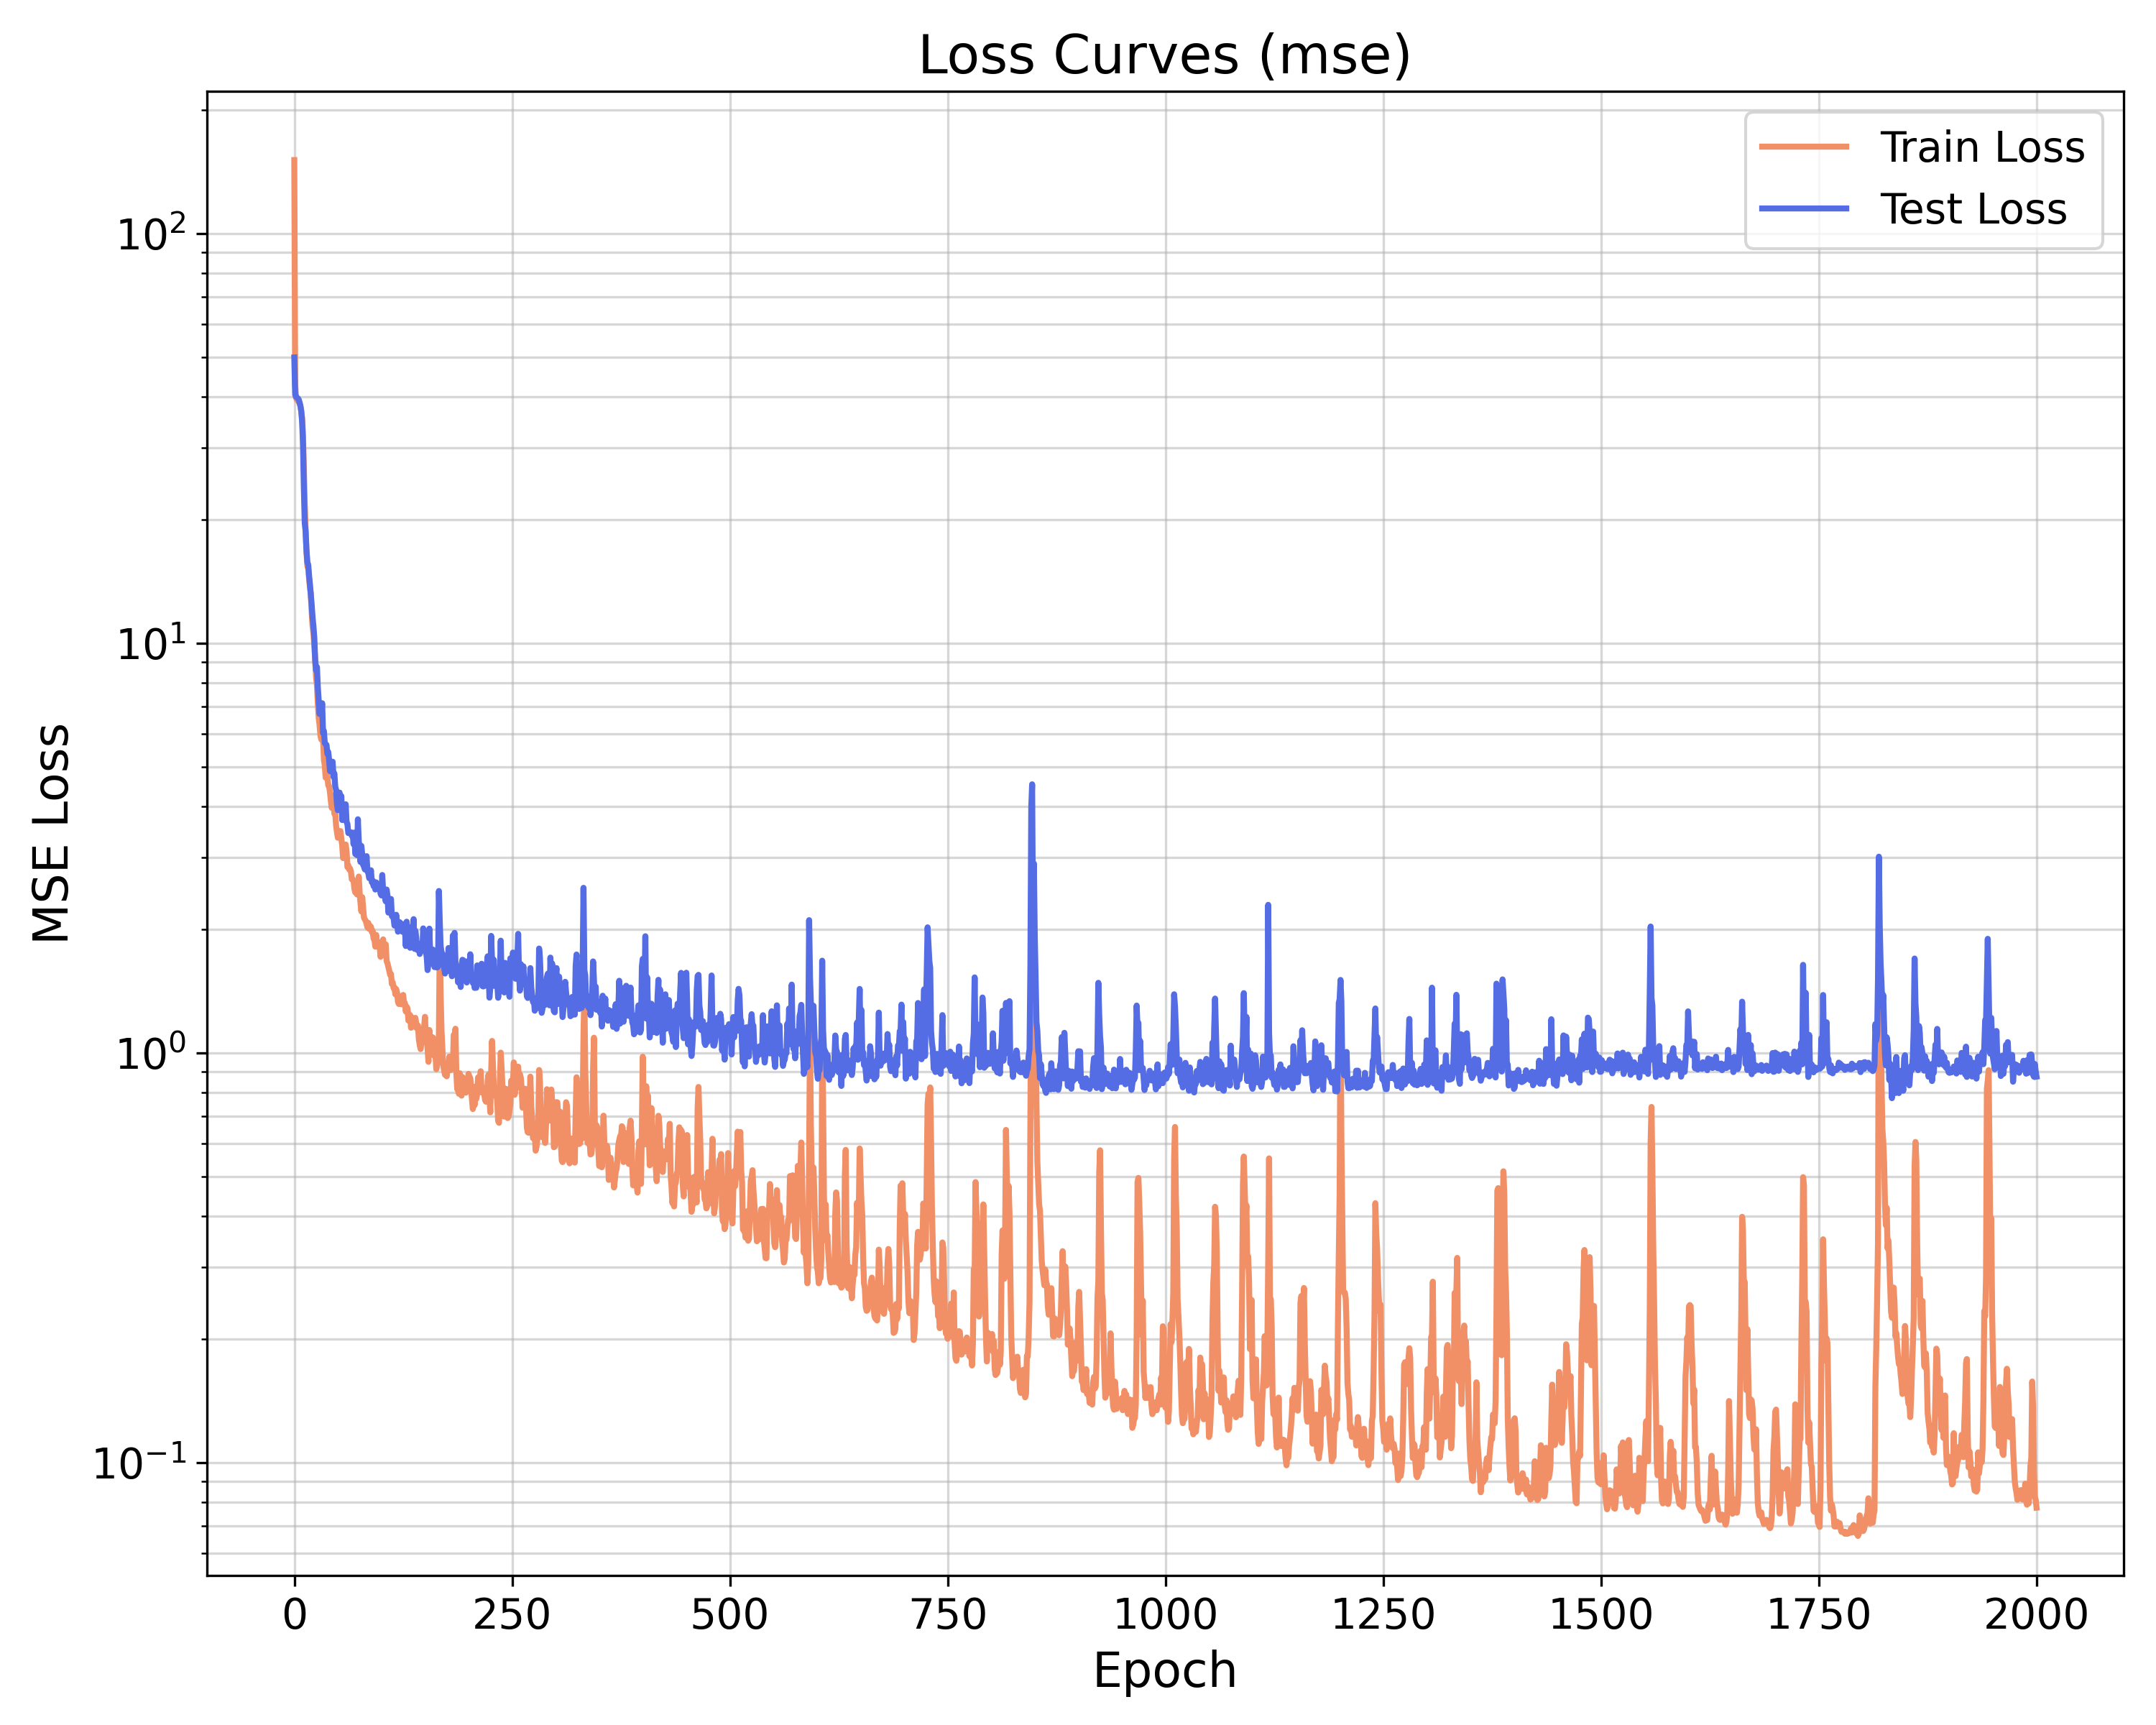
\includegraphics[width=\textwidth]{img/FH_model/ER_Network/FNO/loss_plot_fixed_N=700.png}
        \caption{$N=700$}
    \end{subfigure}
    \hfill
    \begin{subfigure}[b]{0.32\textwidth}
        \centering
        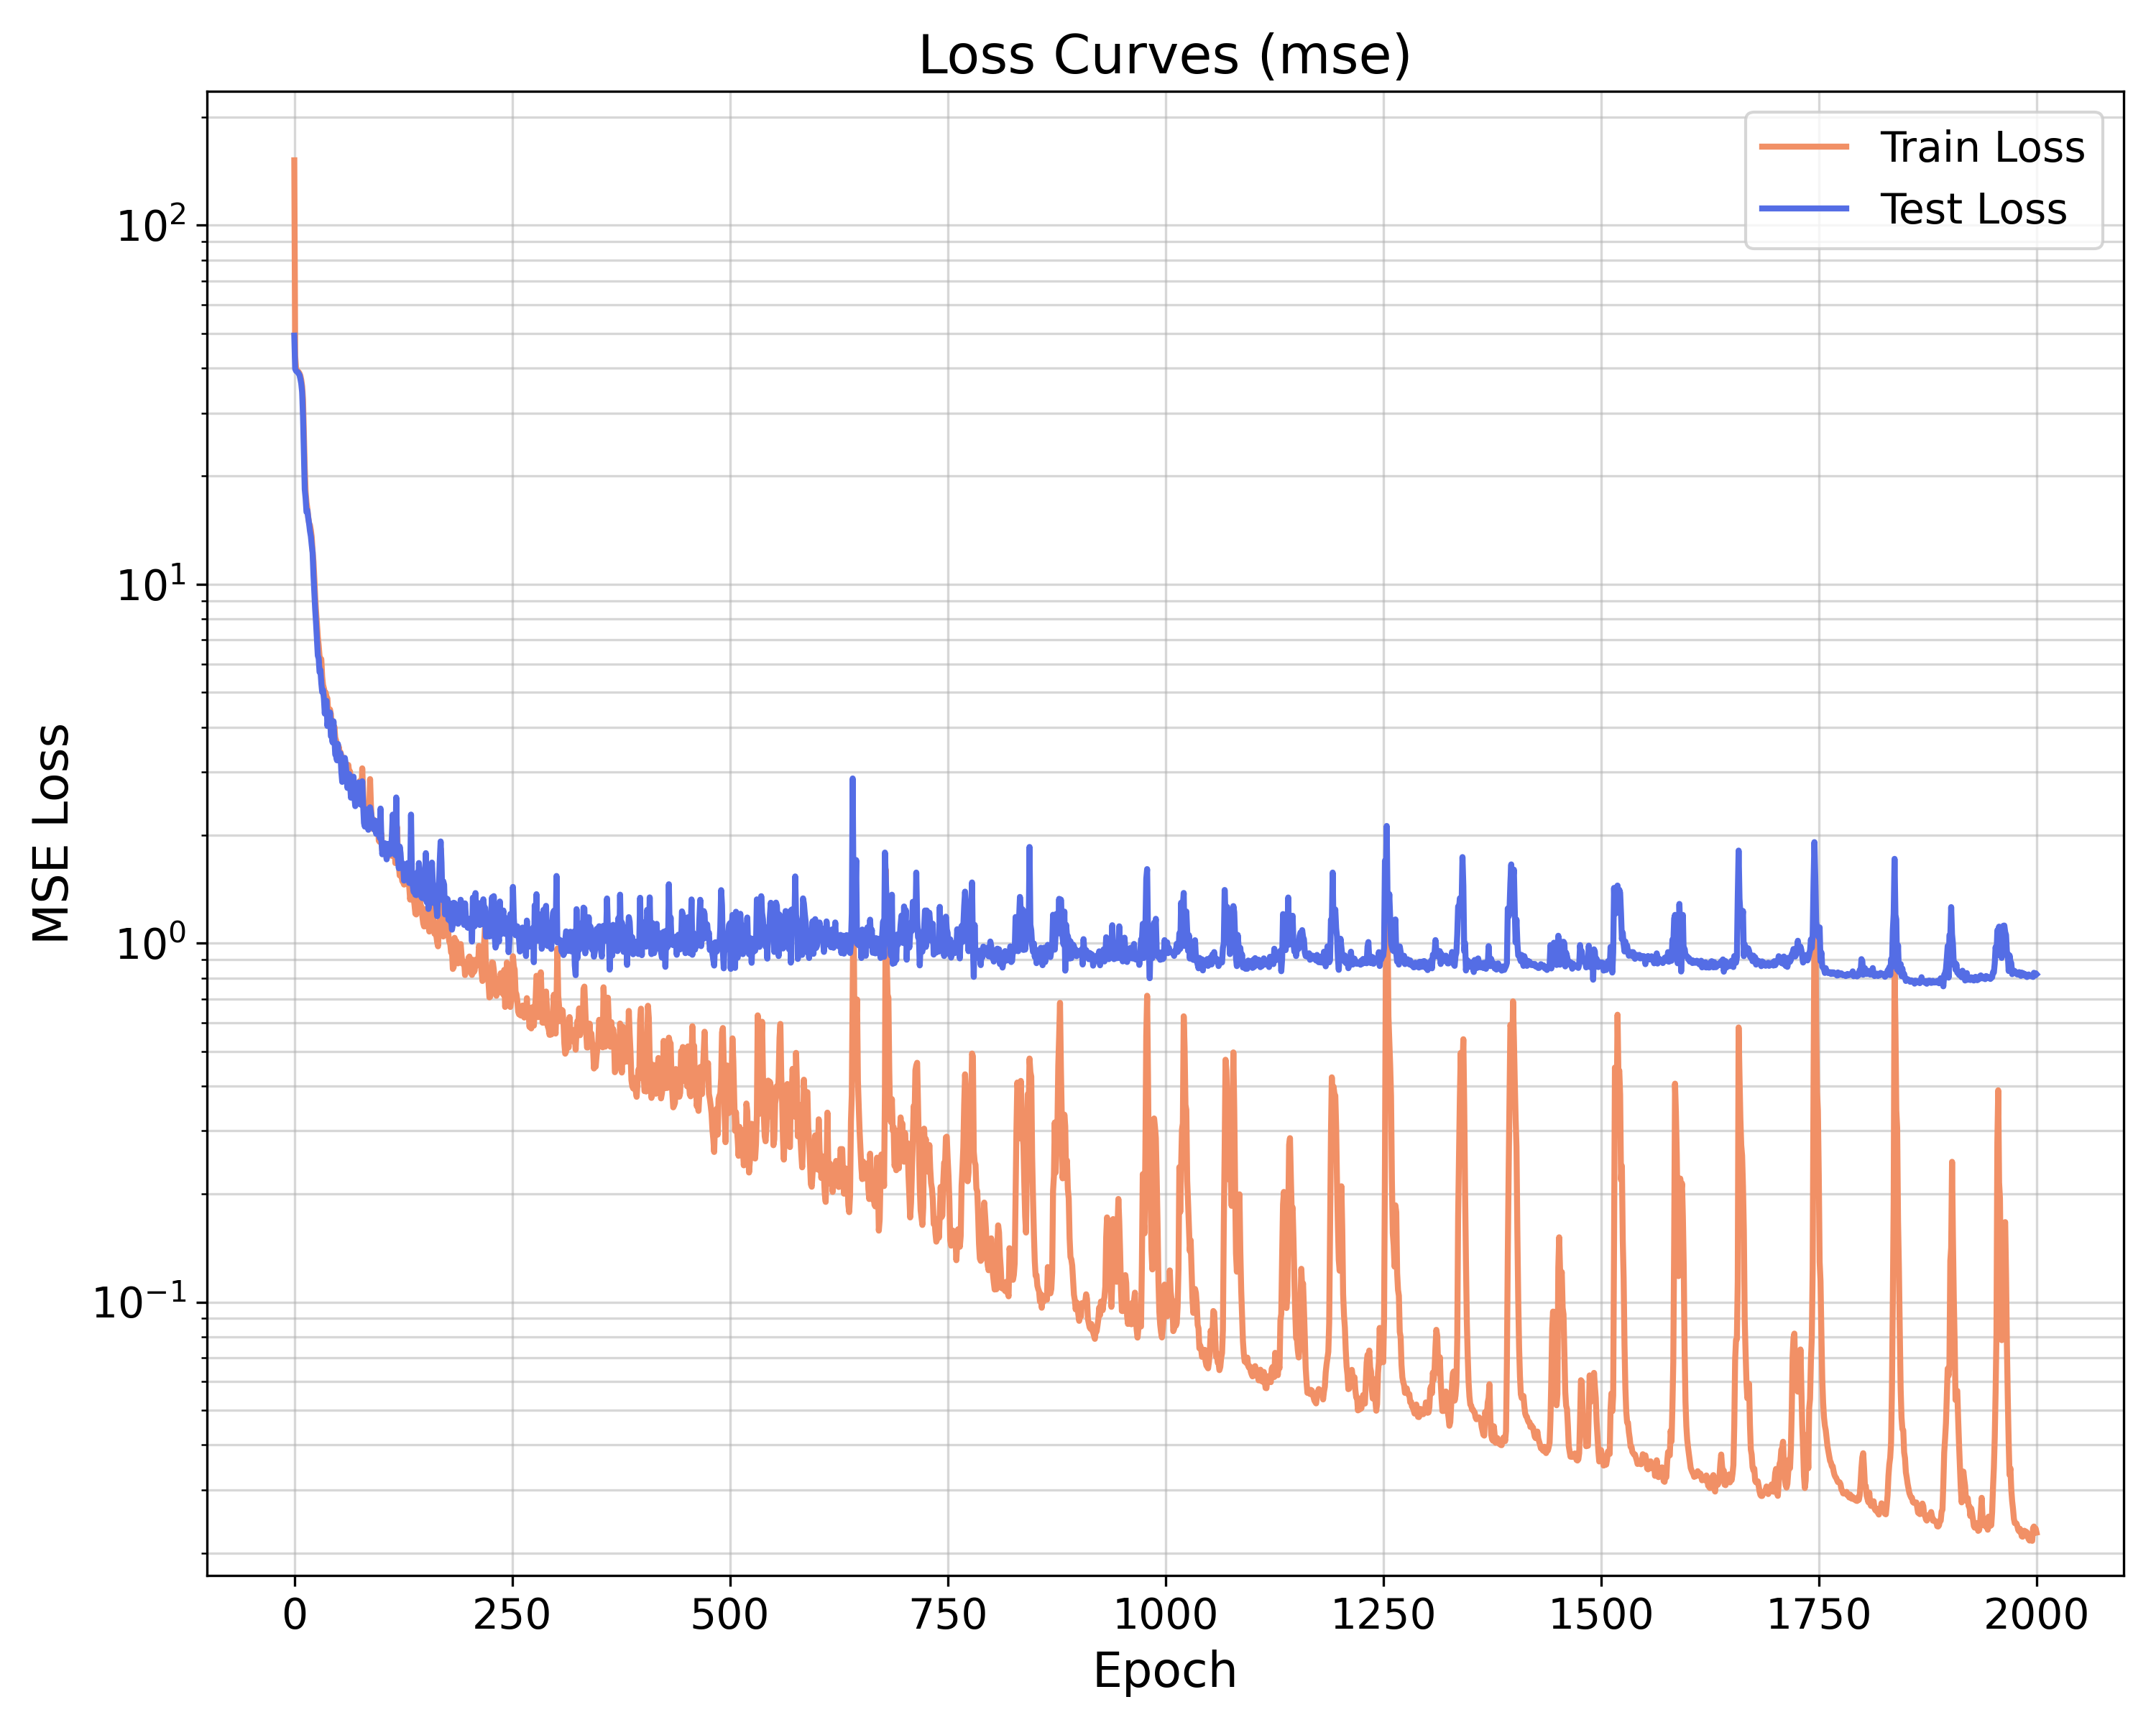
\includegraphics[width=\textwidth]{img/FH_model/ER_Network/FNO/loss_plot_fixed_N=800.png}
        \caption{$N=800$}
    \end{subfigure}
    
    \vspace{0.4cm}
    
    % --- Quarta riga ---
    \begin{subfigure}[b]{0.32\textwidth}
        \centering
        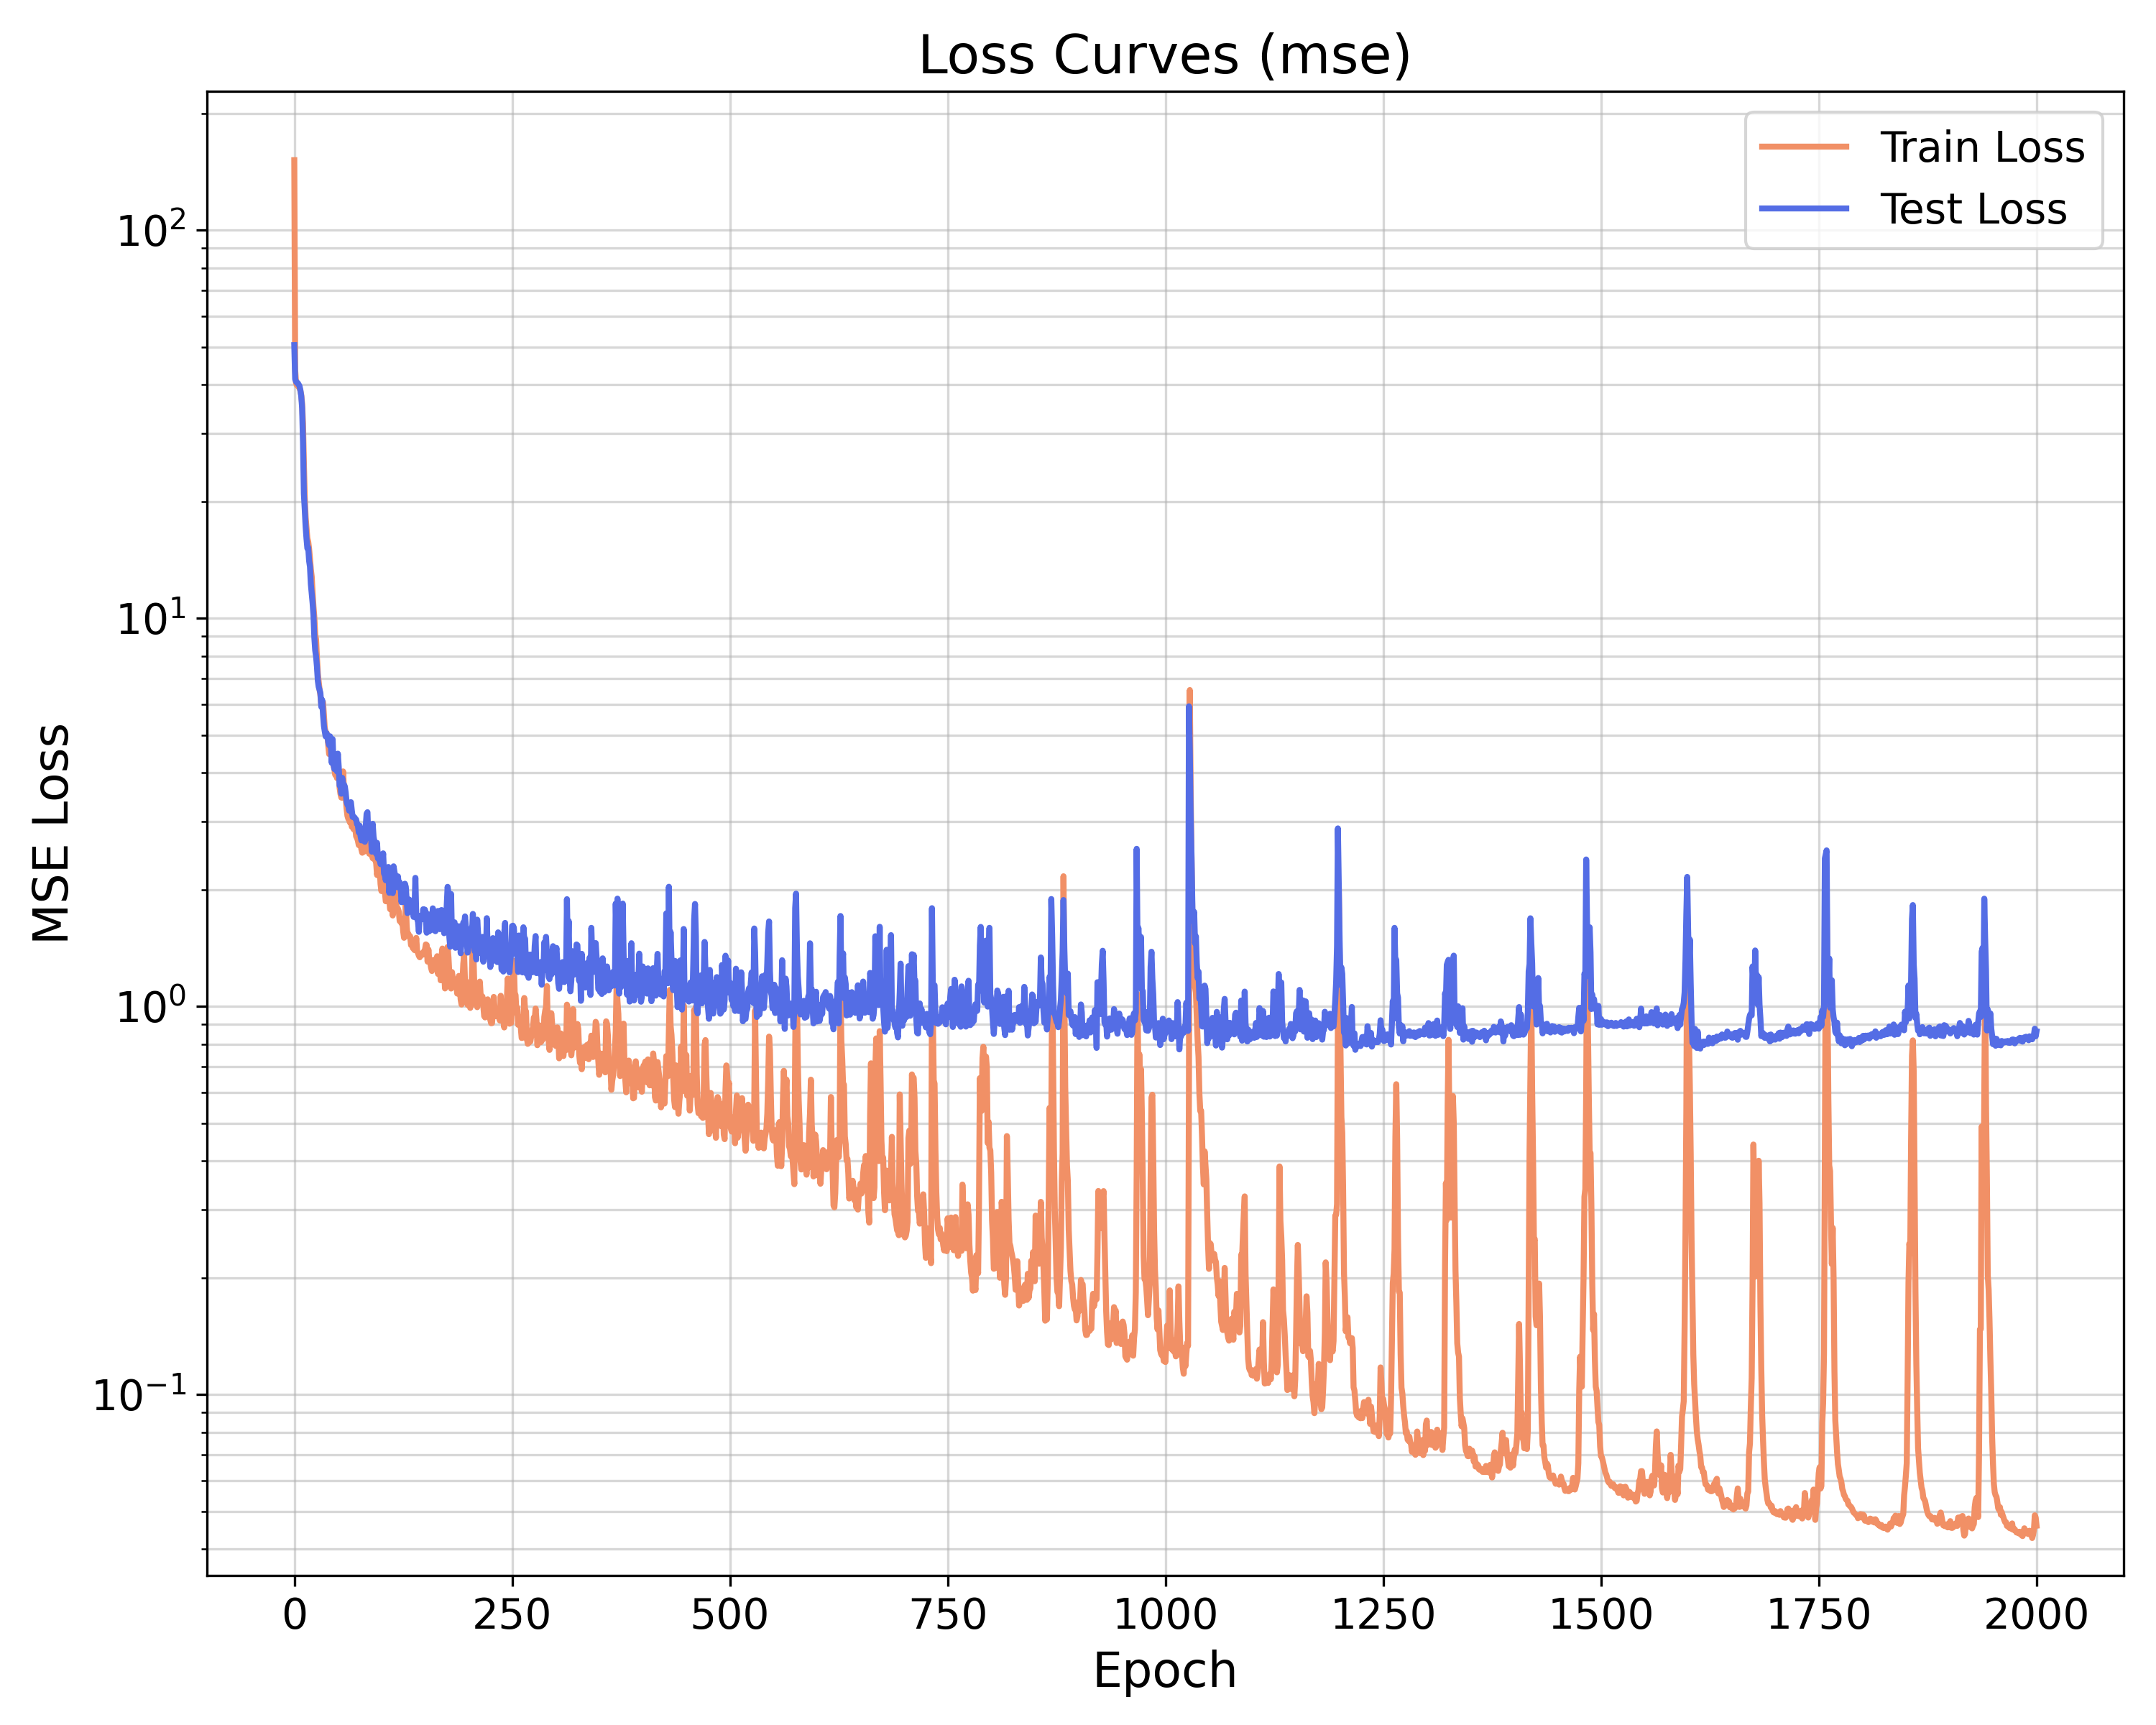
\includegraphics[width=\textwidth]{img/FH_model/ER_Network/FNO/loss_plot_fixed_N=900.png}
        \caption{$N=900$}
    \end{subfigure}
    \hfill
    \begin{subfigure}[b]{0.32\textwidth}
        \centering
        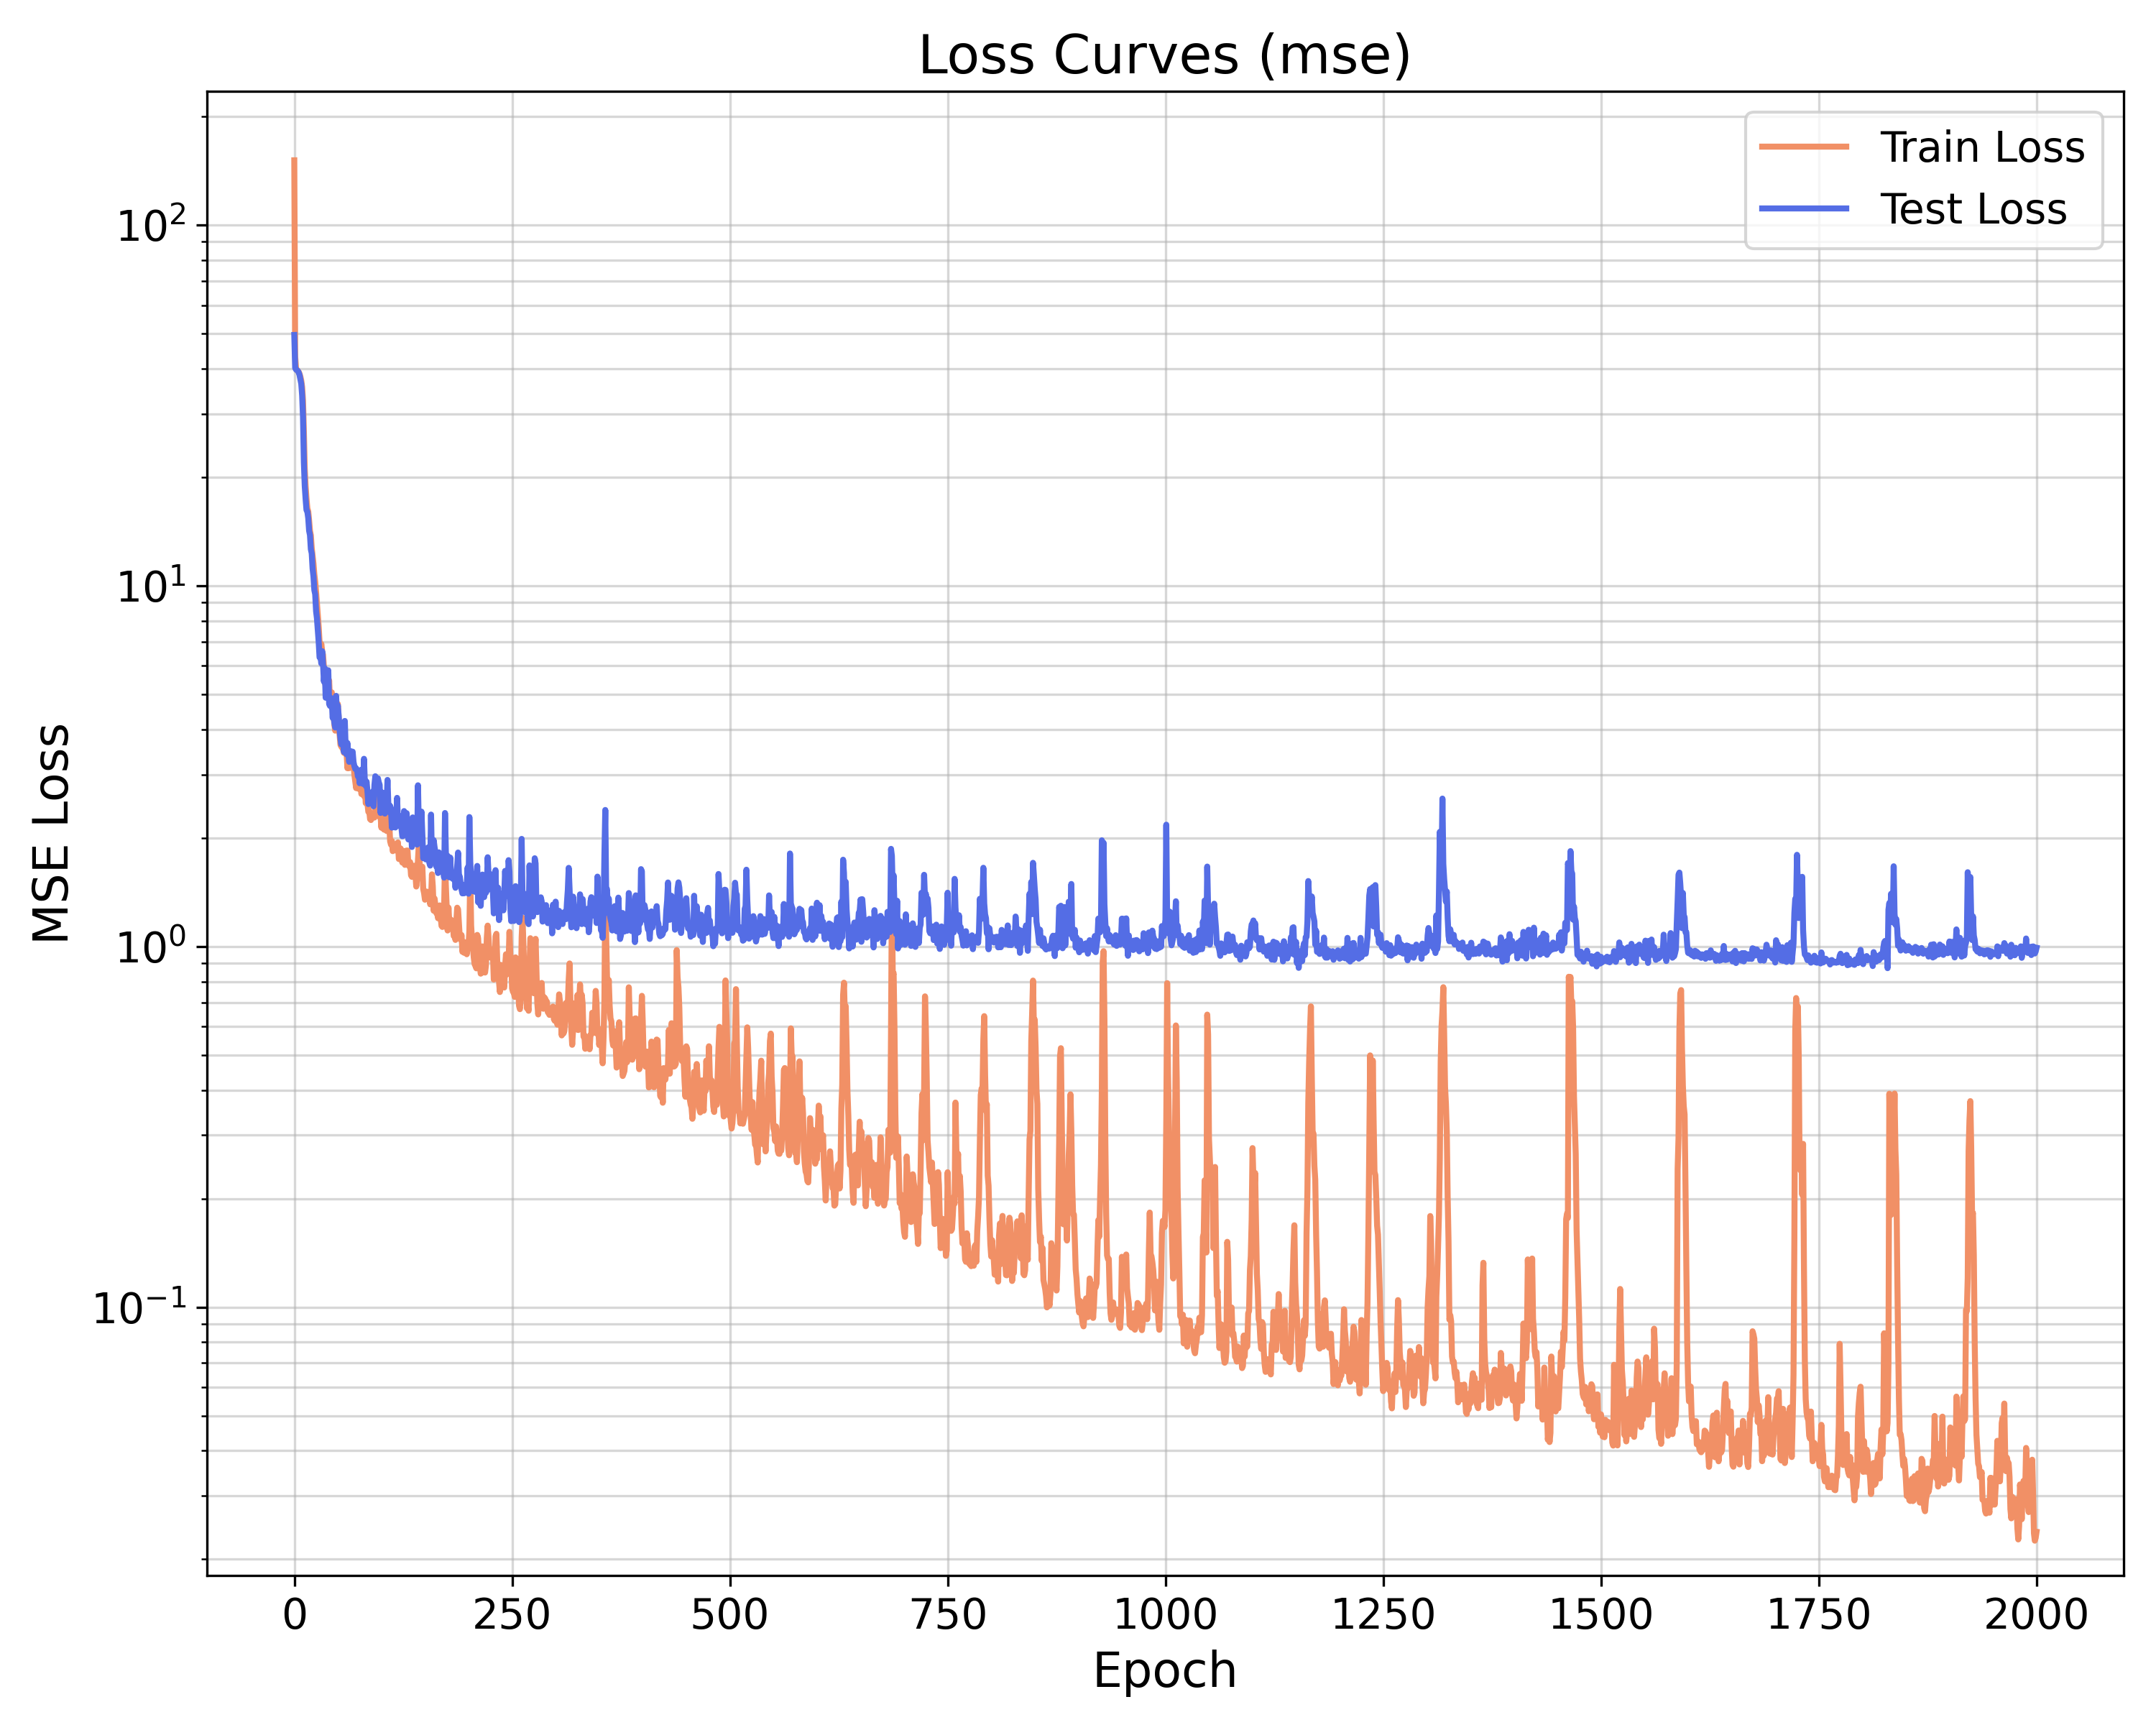
\includegraphics[width=\textwidth]{img/FH_model/ER_Network/FNO/loss_plot_fixed_N=1000.png}
        \caption{$N=1000$}
    \end{subfigure}
    \hfill
    \begin{subfigure}[b]{0.32\textwidth}
        \centering
        
\includegraphics[width=\textwidth]{img/FH_model/ER_Network/FNO/loss_plot_fixed_N=2000.png}
        \caption{$N=2000$}
    \end{subfigure}
    
    \caption{Training and test loss convergence for different Erd\H{o}s-R\'enyi network sizes ($N$).}
    \label{fig:er_loss_grid}
\end{figure}

\subsection{BA network}

Before detailing the results, it is worth briefly recalling that a Barab\'asi-Albert (BA) network is a widely used model for generating random scale-free networks. It relies on a preferential attachment mechanism, meaning that new nodes are more likely to establish connections with existing nodes that already have a high degree.
Due to the particular structure of this family of networks, we defined the hubs as the nodes whose degree exceeds the 95th percentile (representing the top 5\% most connected nodes in the graph). Consequently, we opted to randomly connect the input and output nodes exclusively to one of these hubs.
In this way we greatly reduced the variability of the dynamics due to the seed.

Following the same rationale as the previous section, we proceeded to observe if the performance of FNO degraded with the growing size ($N$) of the hidden network. To conduct this experiment we performed our analysis for different sizes of the BA network: $N= 10,100,200,300,400,500,600,700,800,900,1000,2000$. 
Since the input and output nodes are randomly chosen, we repeated each experiment with different seeds ($0, 42, 100$) to distinguish whether specific effects are intrinsic to the topology or merely due to the chance of the particular sampling of input/output nodes.

Here we reported only figures for the seed $S=42$.

As a representative example of the system's setup, Figure \ref{fig:ba_setup_100} reports the network topology for a BA graph of size $N=100$.

\begin{figure}[htbp]
    \centering
    
\includegraphics[width=\textwidth]{img/FH_model/BA_Network/network_plot_BA_N=100.png}
    \caption{Our setup for a Barab\'asi-Albert network of size $N=100$.}
    \label{fig:ba_setup_100}
\end{figure}


%%%
%%%
% ==========================================
% GRIGLIA 1: PEAKS (Estensione .png)
% ==========================================
\begin{figure}[htbp]
    \centering
    % --- Prima riga ---
    \begin{subfigure}[b]{0.32\textwidth}
        \centering
        
\includegraphics[width=\textwidth]{img/FH_model/BA_Network/FNO/HHpeaks_S=42_N=10.png}
        \caption{$N=10$}
    \end{subfigure}
    \hfill
    \begin{subfigure}[b]{0.32\textwidth}
        \centering
        
\includegraphics[width=\textwidth]{img/FH_model/BA_Network/FNO/HHpeaks_S=42_N=100.png}
        \caption{$N=100$}
    \end{subfigure}
    \hfill
    \begin{subfigure}[b]{0.32\textwidth}
        \centering
        
\includegraphics[width=\textwidth]{img/FH_model/BA_Network/FNO/HHpeaks_S=42_N=200.png}
        \caption{$N=200$}
    \end{subfigure}
    
    \vspace{0.4cm}
    
    % --- Seconda riga ---
    \begin{subfigure}[b]{0.32\textwidth}
        \centering
        
\includegraphics[width=\textwidth]{img/FH_model/BA_Network/FNO/HHpeaks_S=42_N=300.png}
        \caption{$N=300$}
    \end{subfigure}
    \hfill
    \begin{subfigure}[b]{0.32\textwidth}
        \centering
        
\includegraphics[width=\textwidth]{img/FH_model/BA_Network/FNO/HHpeaks_S=42_N=400.png}
        \caption{$N=400$}
    \end{subfigure}
    \hfill
    \begin{subfigure}[b]{0.32\textwidth}
        \centering
        
\includegraphics[width=\textwidth]{img/FH_model/BA_Network/FNO/HHpeaks_S=42_N=500.png}
        \caption{$N=500$}
    \end{subfigure}
    
    \vspace{0.4cm}
    
    % --- Terza riga ---
    \begin{subfigure}[b]{0.32\textwidth}
        \centering
        
\includegraphics[width=\textwidth]{img/FH_model/BA_Network/FNO/HHpeaks_S=42_N=600.png}
        \caption{$N=600$}
    \end{subfigure}
    \hfill
    \begin{subfigure}[b]{0.32\textwidth}
        \centering
        
\includegraphics[width=\textwidth]{img/FH_model/BA_Network/FNO/HHpeaks_S=42_N=700.png}
        \caption{$N=700$}
    \end{subfigure}
    \hfill
    \begin{subfigure}[b]{0.32\textwidth}
        \centering
        
\includegraphics[width=\textwidth]{img/FH_model/BA_Network/FNO/HHpeaks_S=42_N=800.png}
        \caption{$N=800$}
    \end{subfigure}
    
    \vspace{0.4cm}
    
    % --- Quarta riga ---
    \begin{subfigure}[b]{0.32\textwidth}
        \centering
        
\includegraphics[width=\textwidth]{img/FH_model/BA_Network/FNO/HHpeaks_S=42_N=900.png}
        \caption{$N=900$}
    \end{subfigure}
    \hfill
    \begin{subfigure}[b]{0.32\textwidth}
        \centering
        
\includegraphics[width=\textwidth]{img/FH_model/BA_Network/FNO/HHpeaks_S=42_N=1000.png}
        \caption{$N=1000$}
    \end{subfigure}
    \hfill
    \begin{subfigure}[b]{0.32\textwidth}
        \centering
        
\includegraphics[width=\textwidth]{img/FH_model/BA_Network/FNO/HHpeaks_S=42_N=2000.png}
        \caption{$N=2000$}
    \end{subfigure}
    
    \caption{Some instances of the test set for different Barab\'asi-Albert network sizes ($N$). For each column we can see the applied input current (bottom) with its corresponding potential response (top): the blue line represents the result of the simulations, whereas the dotted red line indicates the output of the NN.}
    \label{fig:ba_peaks_grid}
\end{figure}

%%%
% ==========================================
% GRIGLIA 2: MSE HISTOGRAMS (Estensione .png)
% ==========================================

\begin{figure}[htbp]
    \centering
    % --- Prima riga ---
    \begin{subfigure}[b]{0.32\textwidth}
        \centering
        
\includegraphics[width=\textwidth]{img/FH_model/BA_Network/FNO/L2histoFNO_S=42_N=10.png}
        \caption{$N=10$}
    \end{subfigure}
    \hfill
    \begin{subfigure}[b]{0.32\textwidth}
        \centering
        
\includegraphics[width=\textwidth]{img/FH_model/BA_Network/FNO/L2histoFNO_S=42_N=100.png}
        \caption{$N=100$}
    \end{subfigure}
    \hfill
    \begin{subfigure}[b]{0.32\textwidth}
        \centering
        
\includegraphics[width=\textwidth]{img/FH_model/BA_Network/FNO/L2histoFNO_S=42_N=200.png}
        \caption{$N=200$}
    \end{subfigure}
    
    \vspace{0.4cm}
    
    % --- Seconda riga ---
    \begin{subfigure}[b]{0.32\textwidth}
        \centering
        
\includegraphics[width=\textwidth]{img/FH_model/BA_Network/FNO/L2histoFNO_S=42_N=300.png}
        \caption{$N=300$}
    \end{subfigure}
    \hfill
    \begin{subfigure}[b]{0.32\textwidth}
        \centering
        
\includegraphics[width=\textwidth]{img/FH_model/BA_Network/FNO/L2histoFNO_S=42_N=400.png}
        \caption{$N=400$}
    \end{subfigure}
    \hfill
    \begin{subfigure}[b]{0.32\textwidth}
        \centering
        
\includegraphics[width=\textwidth]{img/FH_model/BA_Network/FNO/L2histoFNO_S=42_N=500.png}
        \caption{$N=500$}
    \end{subfigure}
    
    \vspace{0.4cm}
    
    % --- Terza riga ---
    \begin{subfigure}[b]{0.32\textwidth}
        \centering
        
\includegraphics[width=\textwidth]{img/FH_model/BA_Network/FNO/L2histoFNO_S=42_N=600.png}
        \caption{$N=600$}
    \end{subfigure}
    \hfill
    \begin{subfigure}[b]{0.32\textwidth}
        \centering
        
\includegraphics[width=\textwidth]{img/FH_model/BA_Network/FNO/L2histoFNO_S=42_N=700.png}
        \caption{$N=700$}
    \end{subfigure}
    \hfill
    \begin{subfigure}[b]{0.32\textwidth}
        \centering
        
\includegraphics[width=\textwidth]{img/FH_model/BA_Network/FNO/L2histoFNO_S=42_N=800.png}
        \caption{$N=800$}
    \end{subfigure}
    
    \vspace{0.4cm}
    
    % --- Quarta riga ---
    \begin{subfigure}[b]{0.32\textwidth}
        \centering
        
\includegraphics[width=\textwidth]{img/FH_model/BA_Network/FNO/L2histoFNO_S=42_N=900.png}
        \caption{$N=900$}
    \end{subfigure}
    \hfill
    \begin{subfigure}[b]{0.32\textwidth}
        \centering
        
\includegraphics[width=\textwidth]{img/FH_model/BA_Network/FNO/L2histoFNO_S=42_N=1000.png}
        \caption{$N=1000$}
    \end{subfigure}
    \hfill
    \begin{subfigure}[b]{0.32\textwidth}
        \centering
        
\includegraphics[width=\textwidth]{img/FH_model/BA_Network/FNO/L2histoFNO_S=42_N=2000.png}
        \caption{$N=2000$}
    \end{subfigure}
    
    \caption{MSE error distributions across the test set for different Barab\'asi-Albert network sizes ($N$).}
    \label{fig:ba_histo_grid}
\end{figure}

% ==========================================
% GRIGLIA 3: LOSS PLOTS (Estensione .png)
% ==========================================
\begin{figure}[htbp]
    \centering
    % --- Prima riga ---
    \begin{subfigure}[b]{0.32\textwidth}
        \centering
        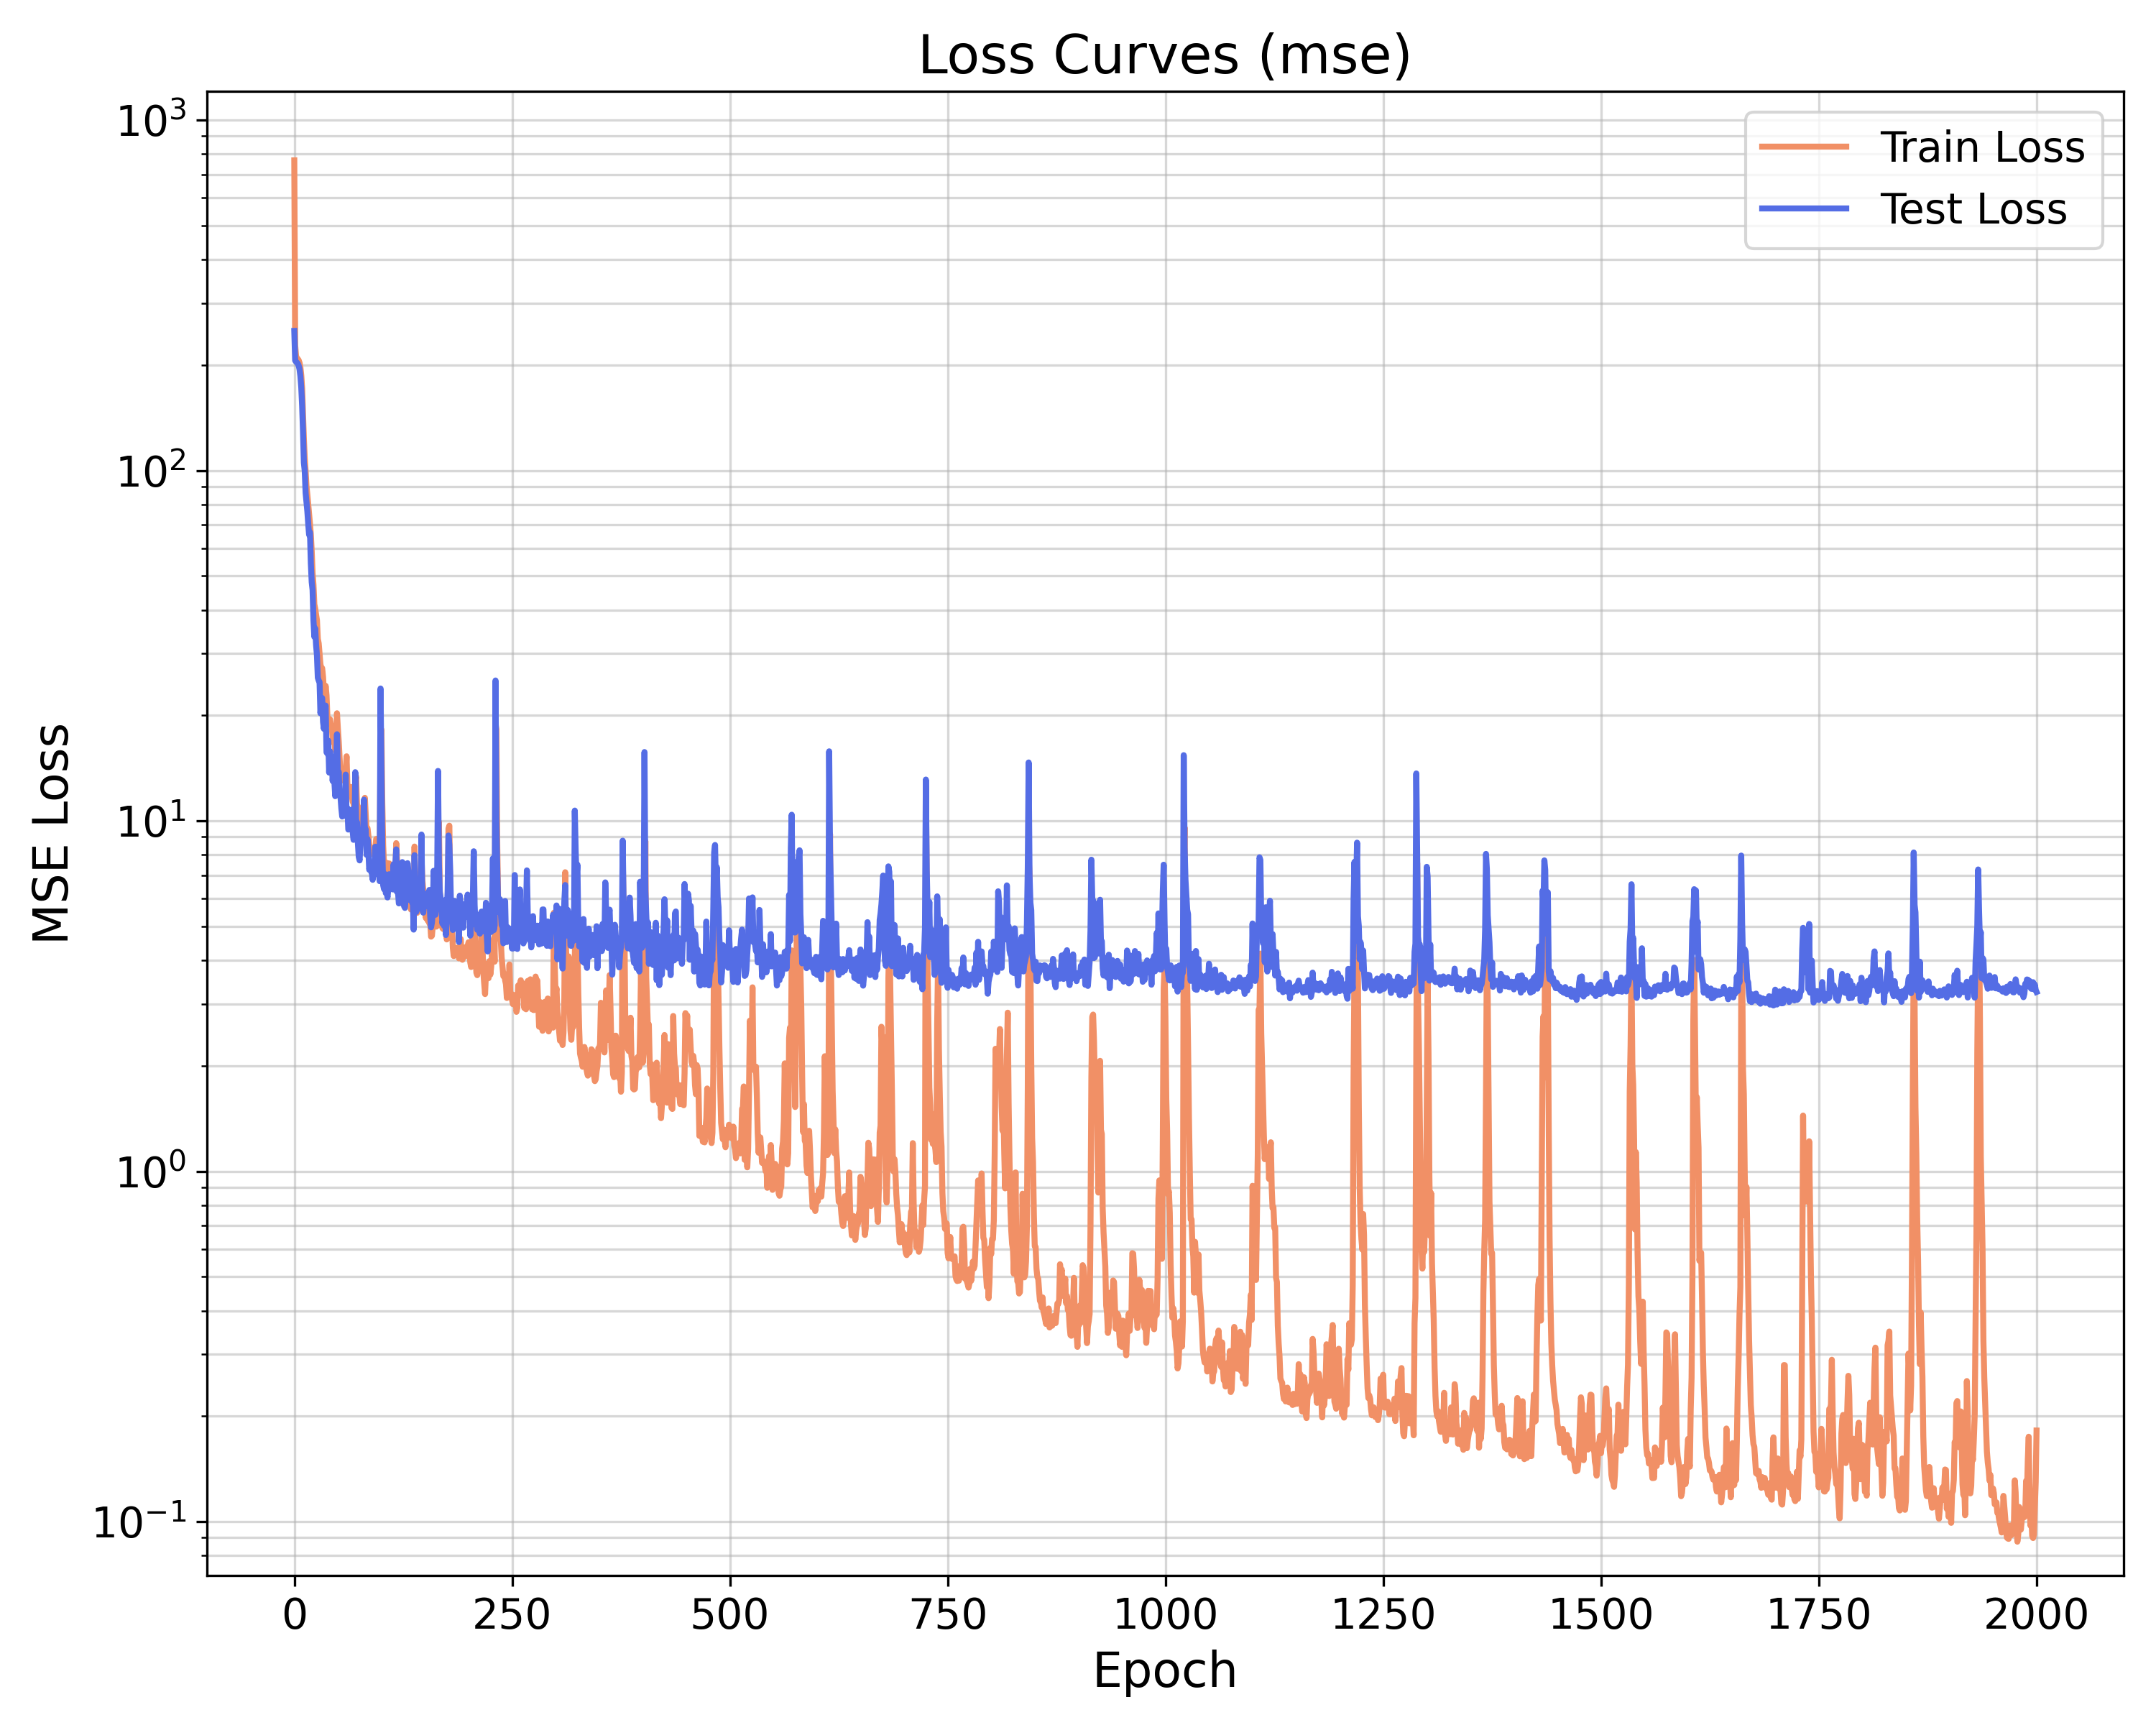
\includegraphics[width=\textwidth]{img/FH_model/BA_Network/FNO/loss_plot_fixed_S=42_N=10.png}
        \caption{$N=10$}
    \end{subfigure}
    \hfill
    \begin{subfigure}[b]{0.32\textwidth}
        \centering
        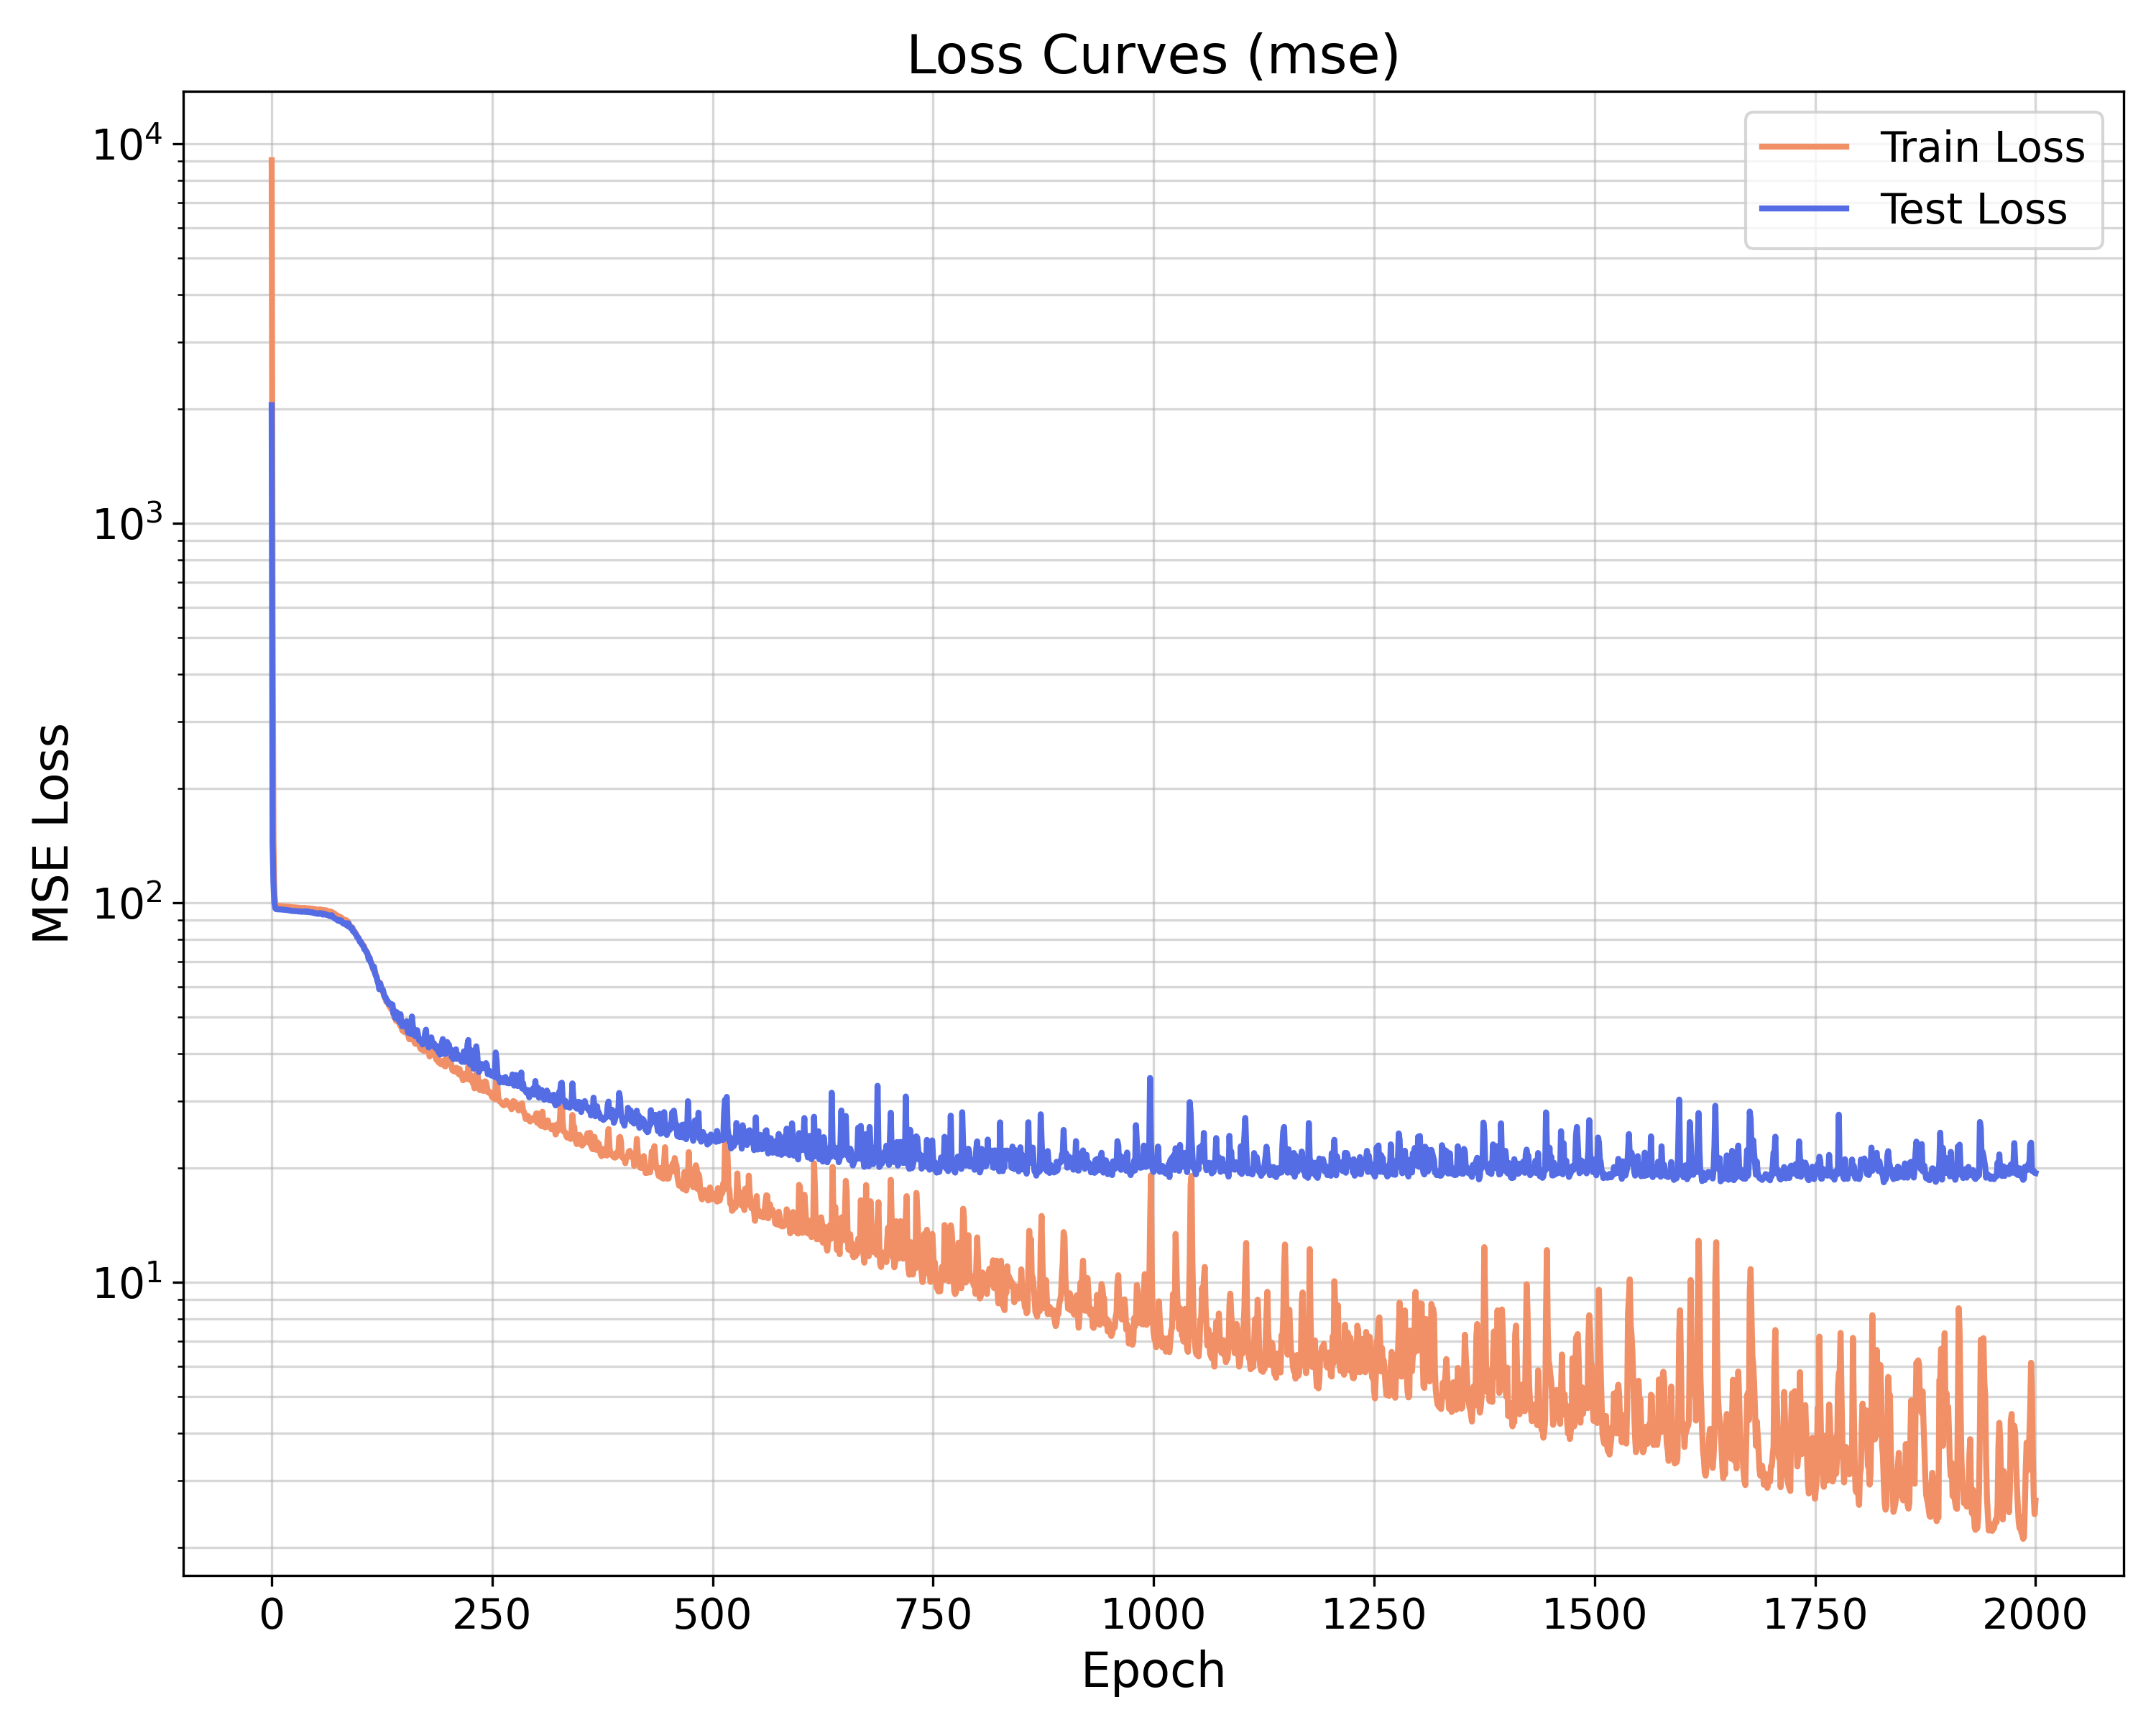
\includegraphics[width=\textwidth]{img/FH_model/BA_Network/FNO/loss_plot_fixed_S=42_N=100.png}
        \caption{$N=100$}
    \end{subfigure}
    \hfill
    \begin{subfigure}[b]{0.32\textwidth}
        \centering
        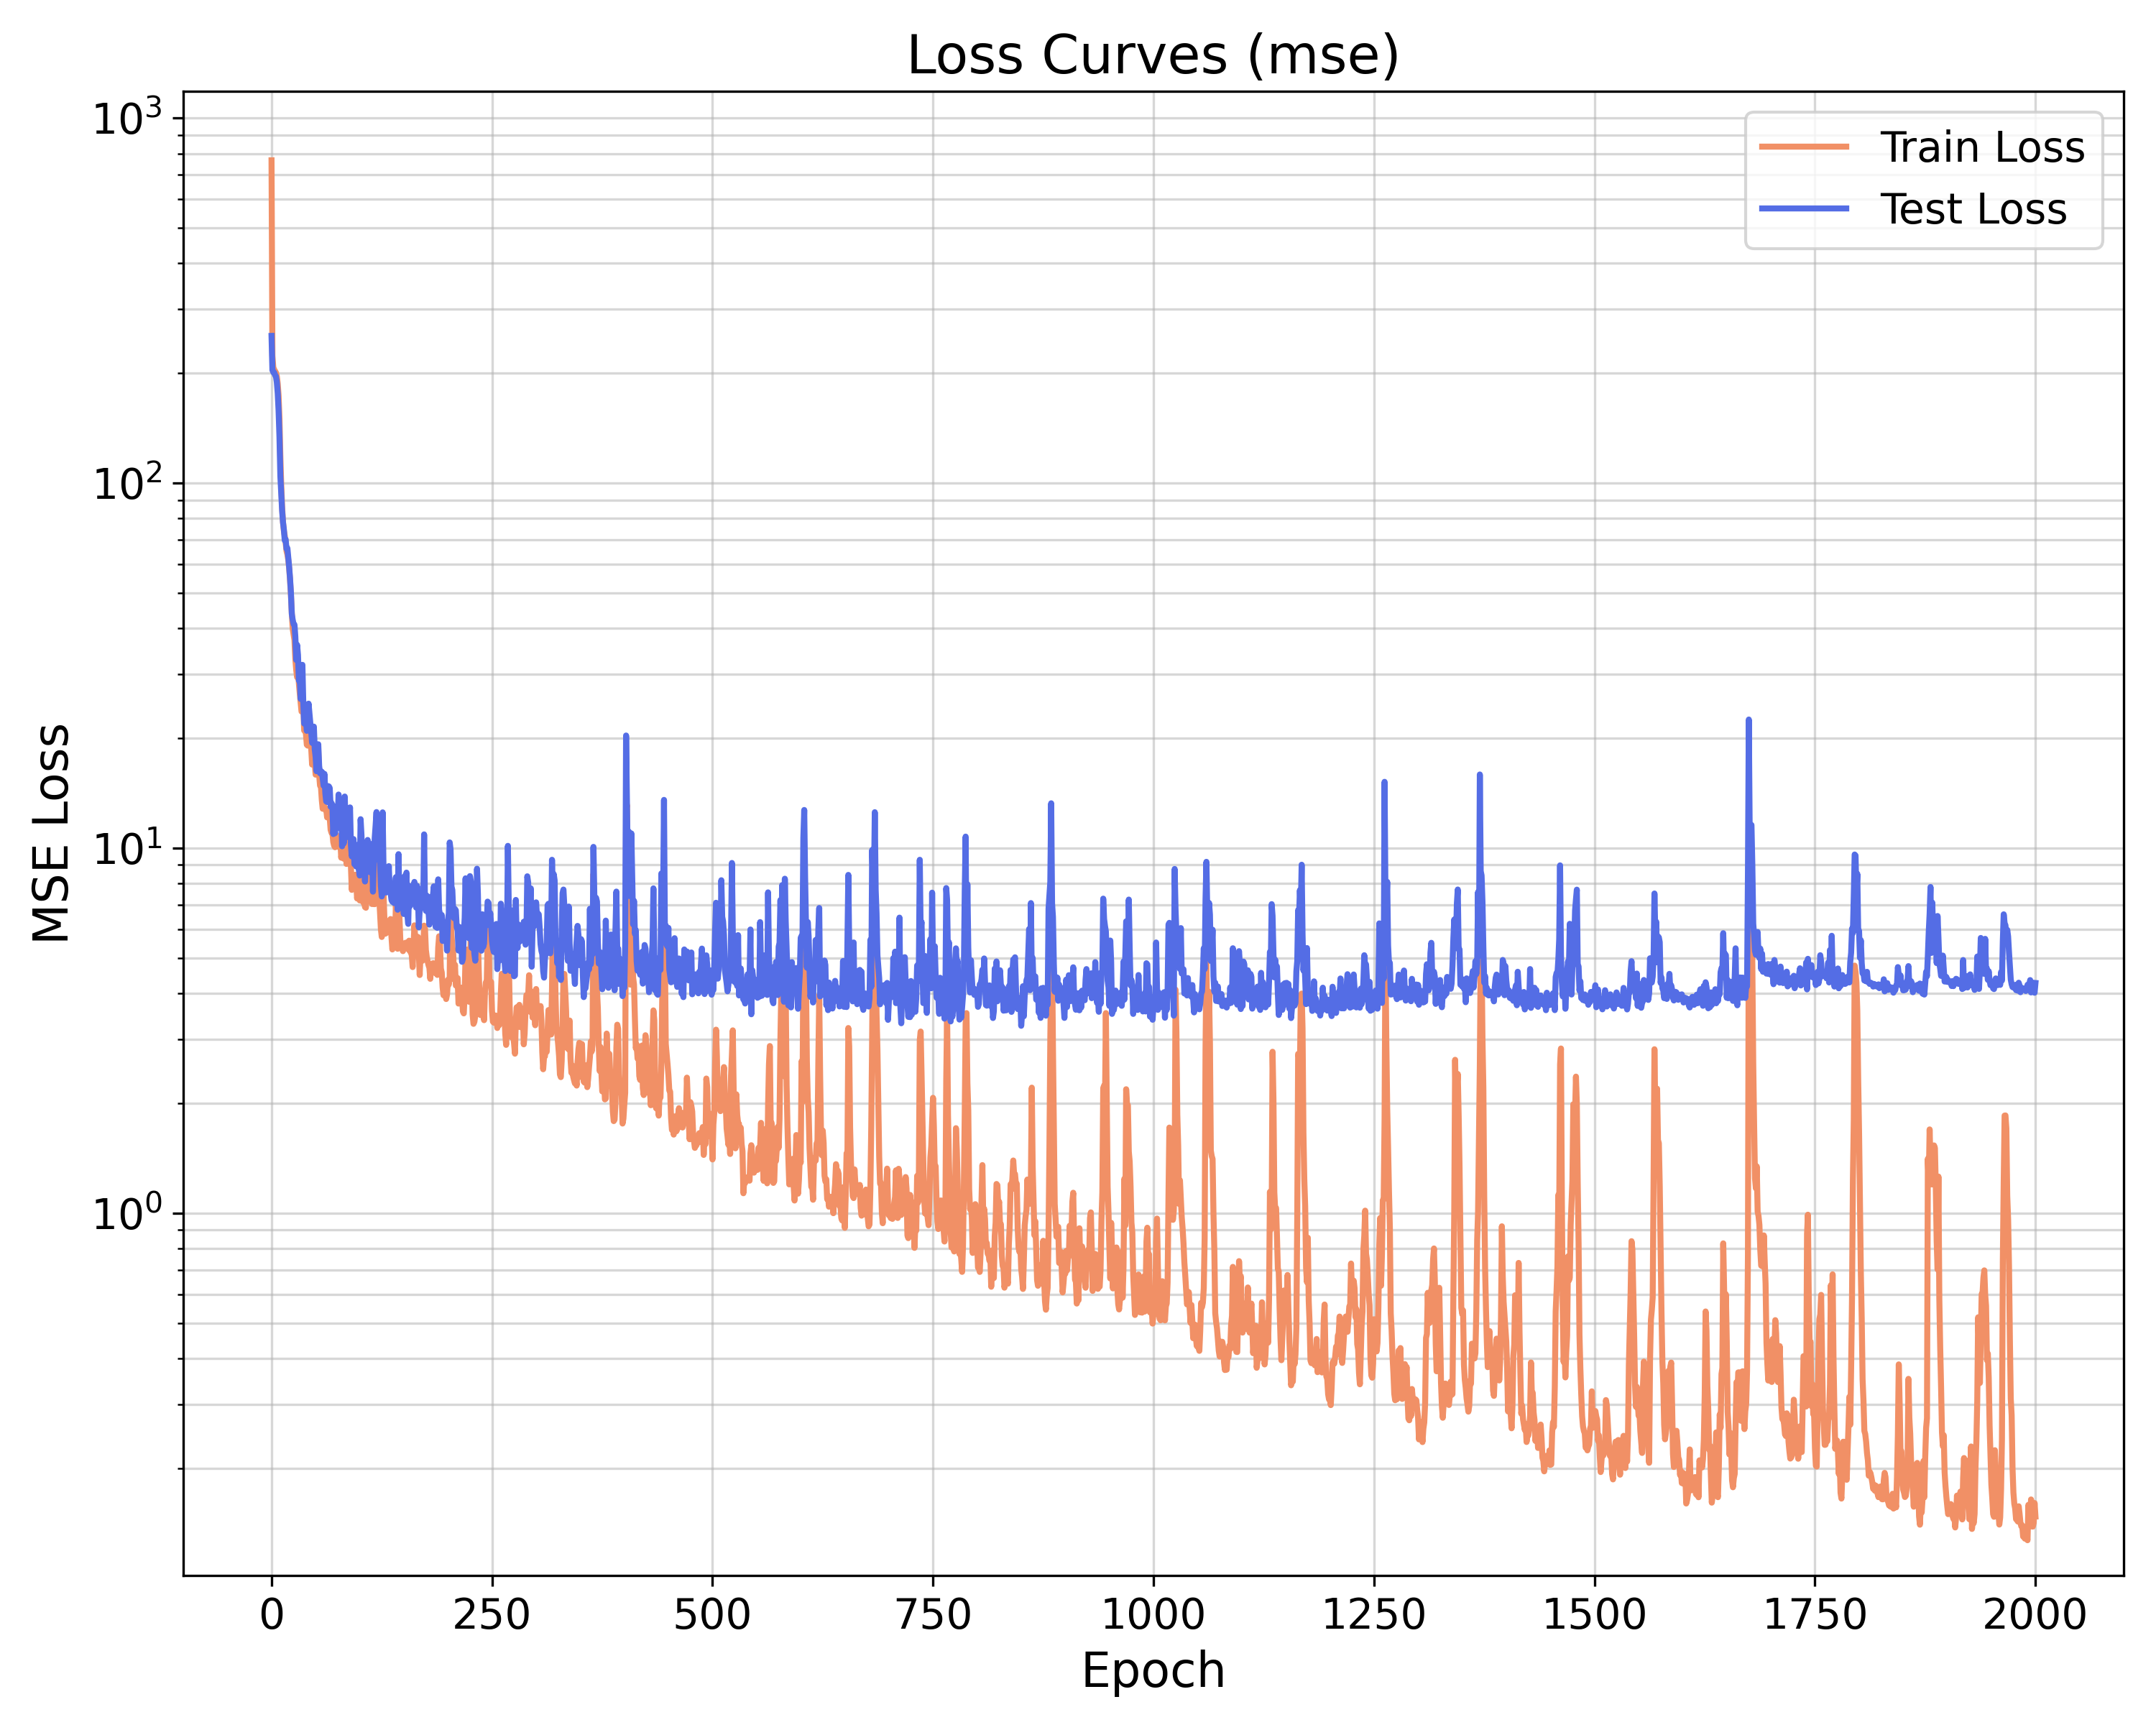
\includegraphics[width=\textwidth]{img/FH_model/BA_Network/FNO/loss_plot_fixed_S=42_N=200.png}
        \caption{$N=200$}
    \end{subfigure}
    
    \vspace{0.4cm}
    
    % --- Seconda riga ---
    \begin{subfigure}[b]{0.32\textwidth}
        \centering
        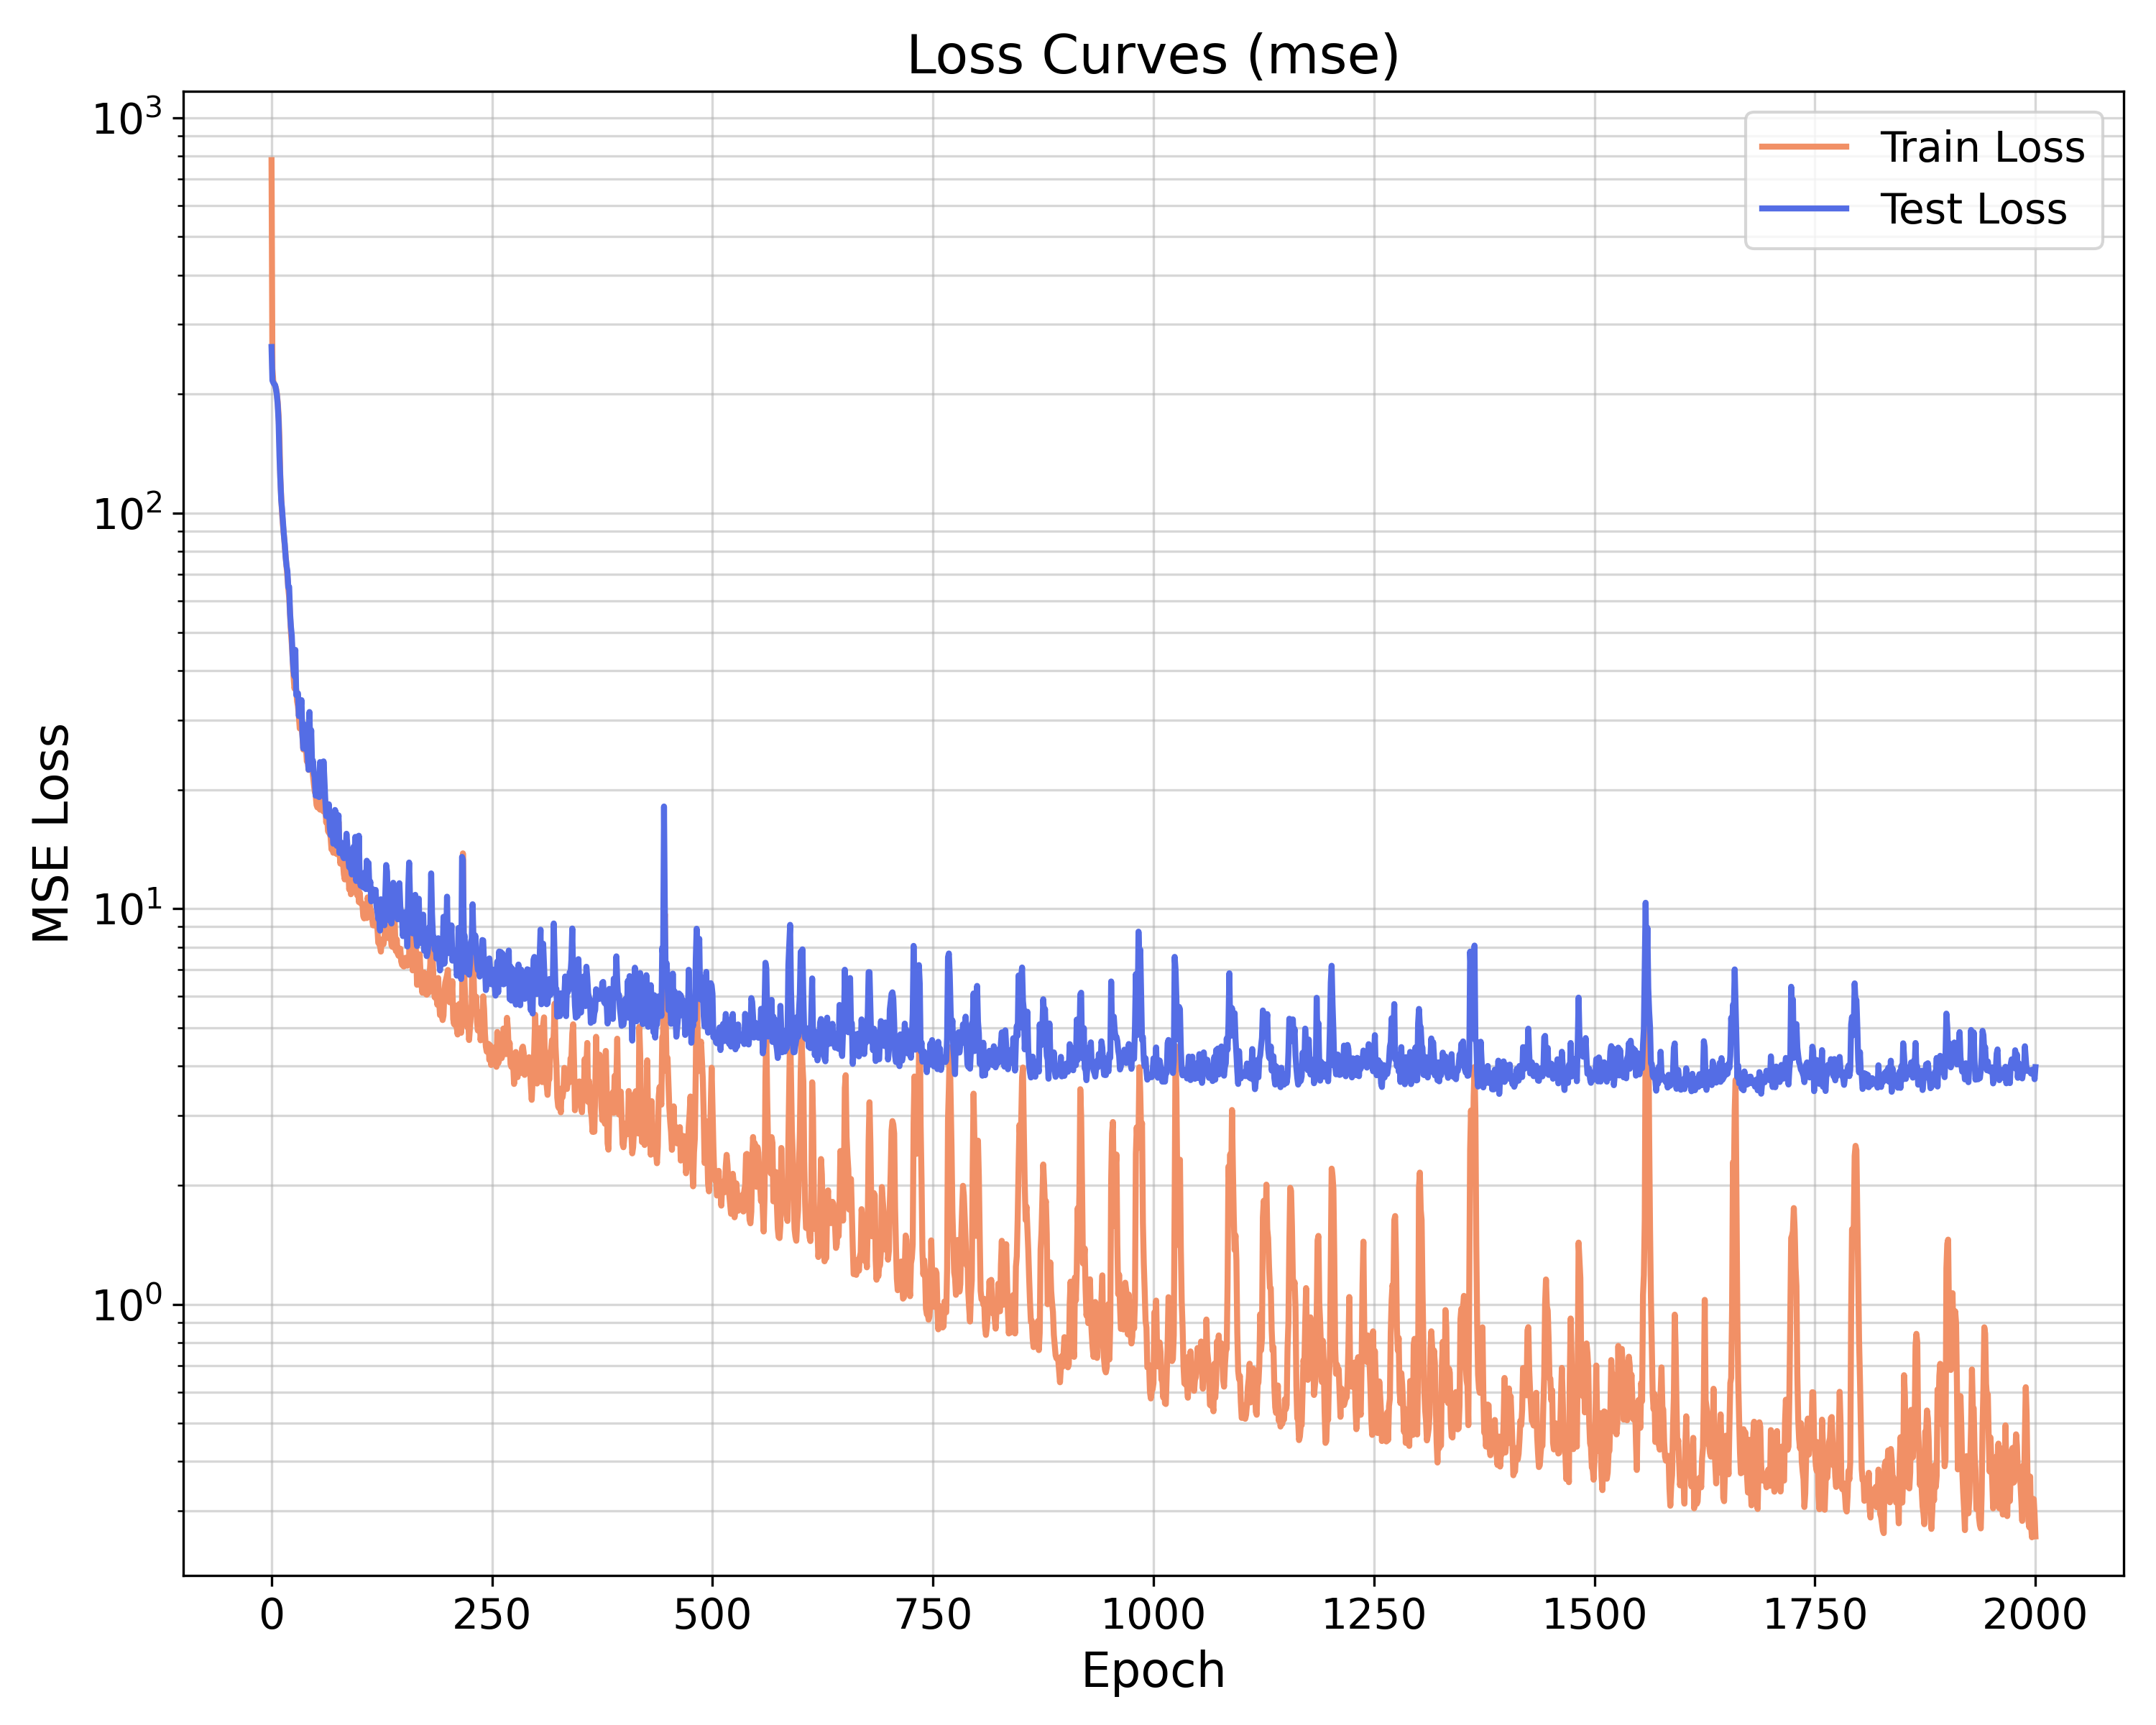
\includegraphics[width=\textwidth]{img/FH_model/BA_Network/FNO/loss_plot_fixed_S=42_N=300.png}
        \caption{$N=300$}
    \end{subfigure}
    \hfill
    \begin{subfigure}[b]{0.32\textwidth}
        \centering
        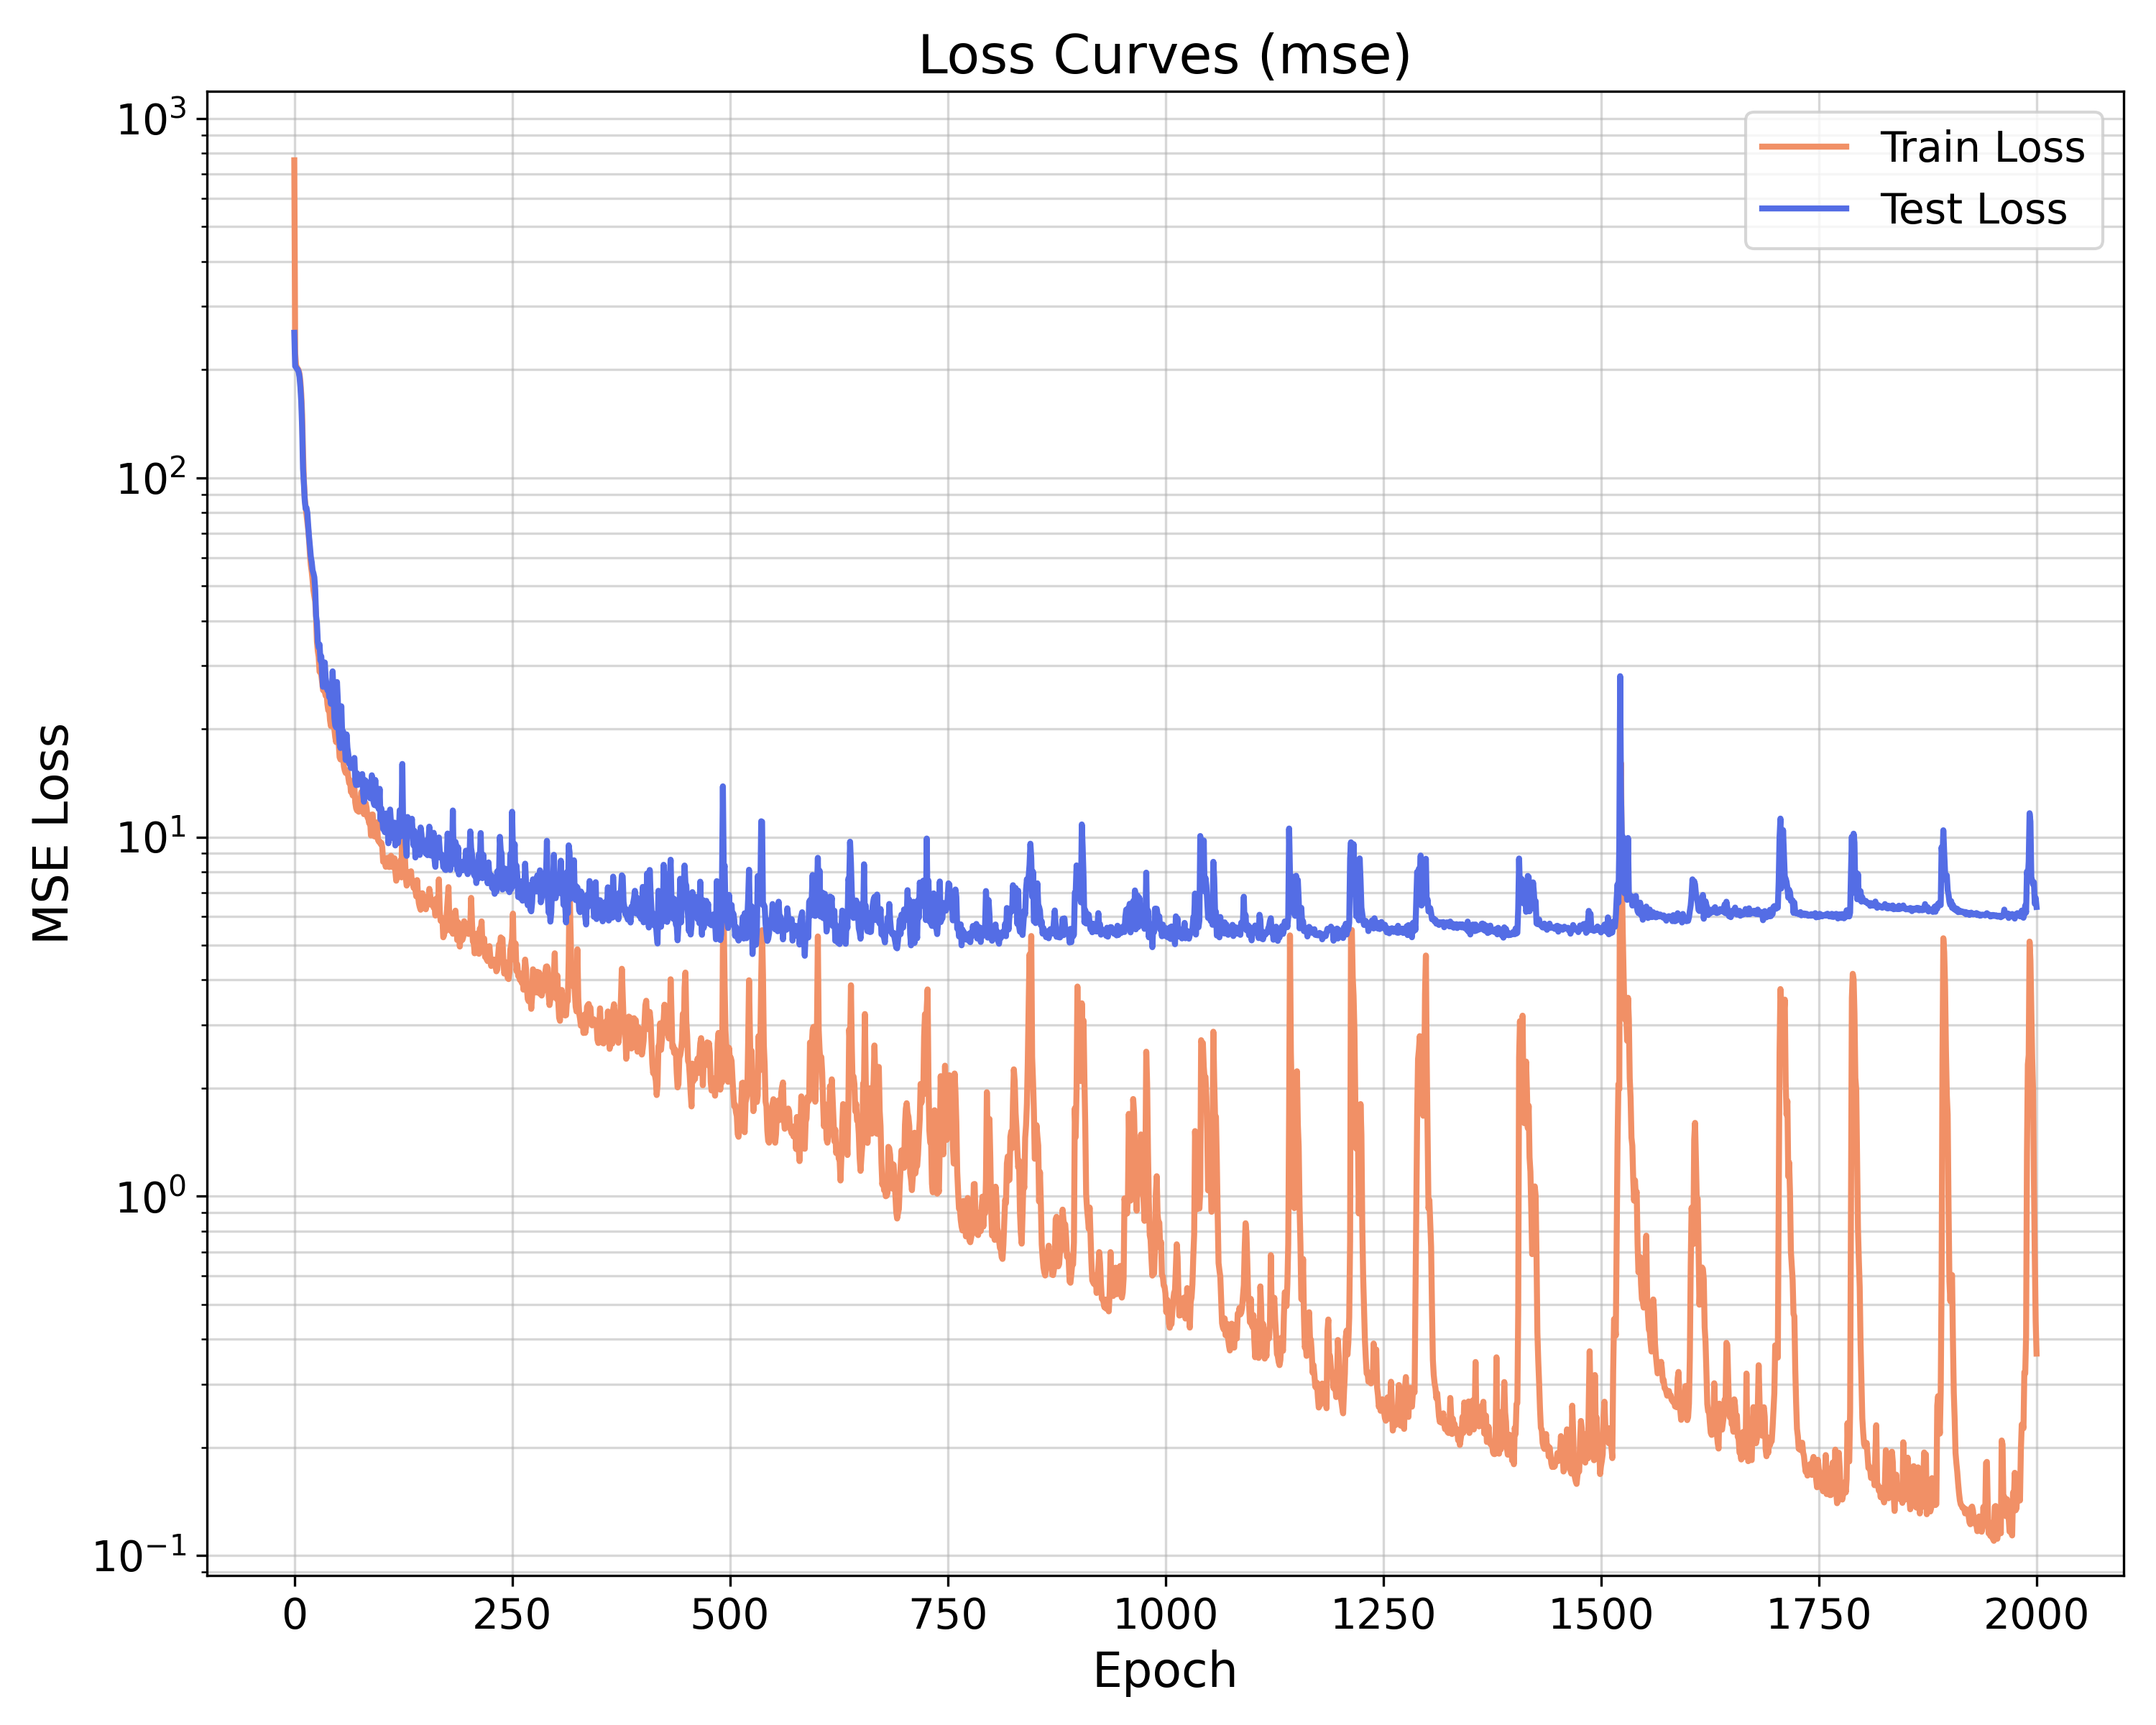
\includegraphics[width=\textwidth]{img/FH_model/BA_Network/FNO/loss_plot_fixed_S=42_N=400.png}
        \caption{$N=400$}
    \end{subfigure}
    \hfill
    \begin{subfigure}[b]{0.32\textwidth}
        \centering
        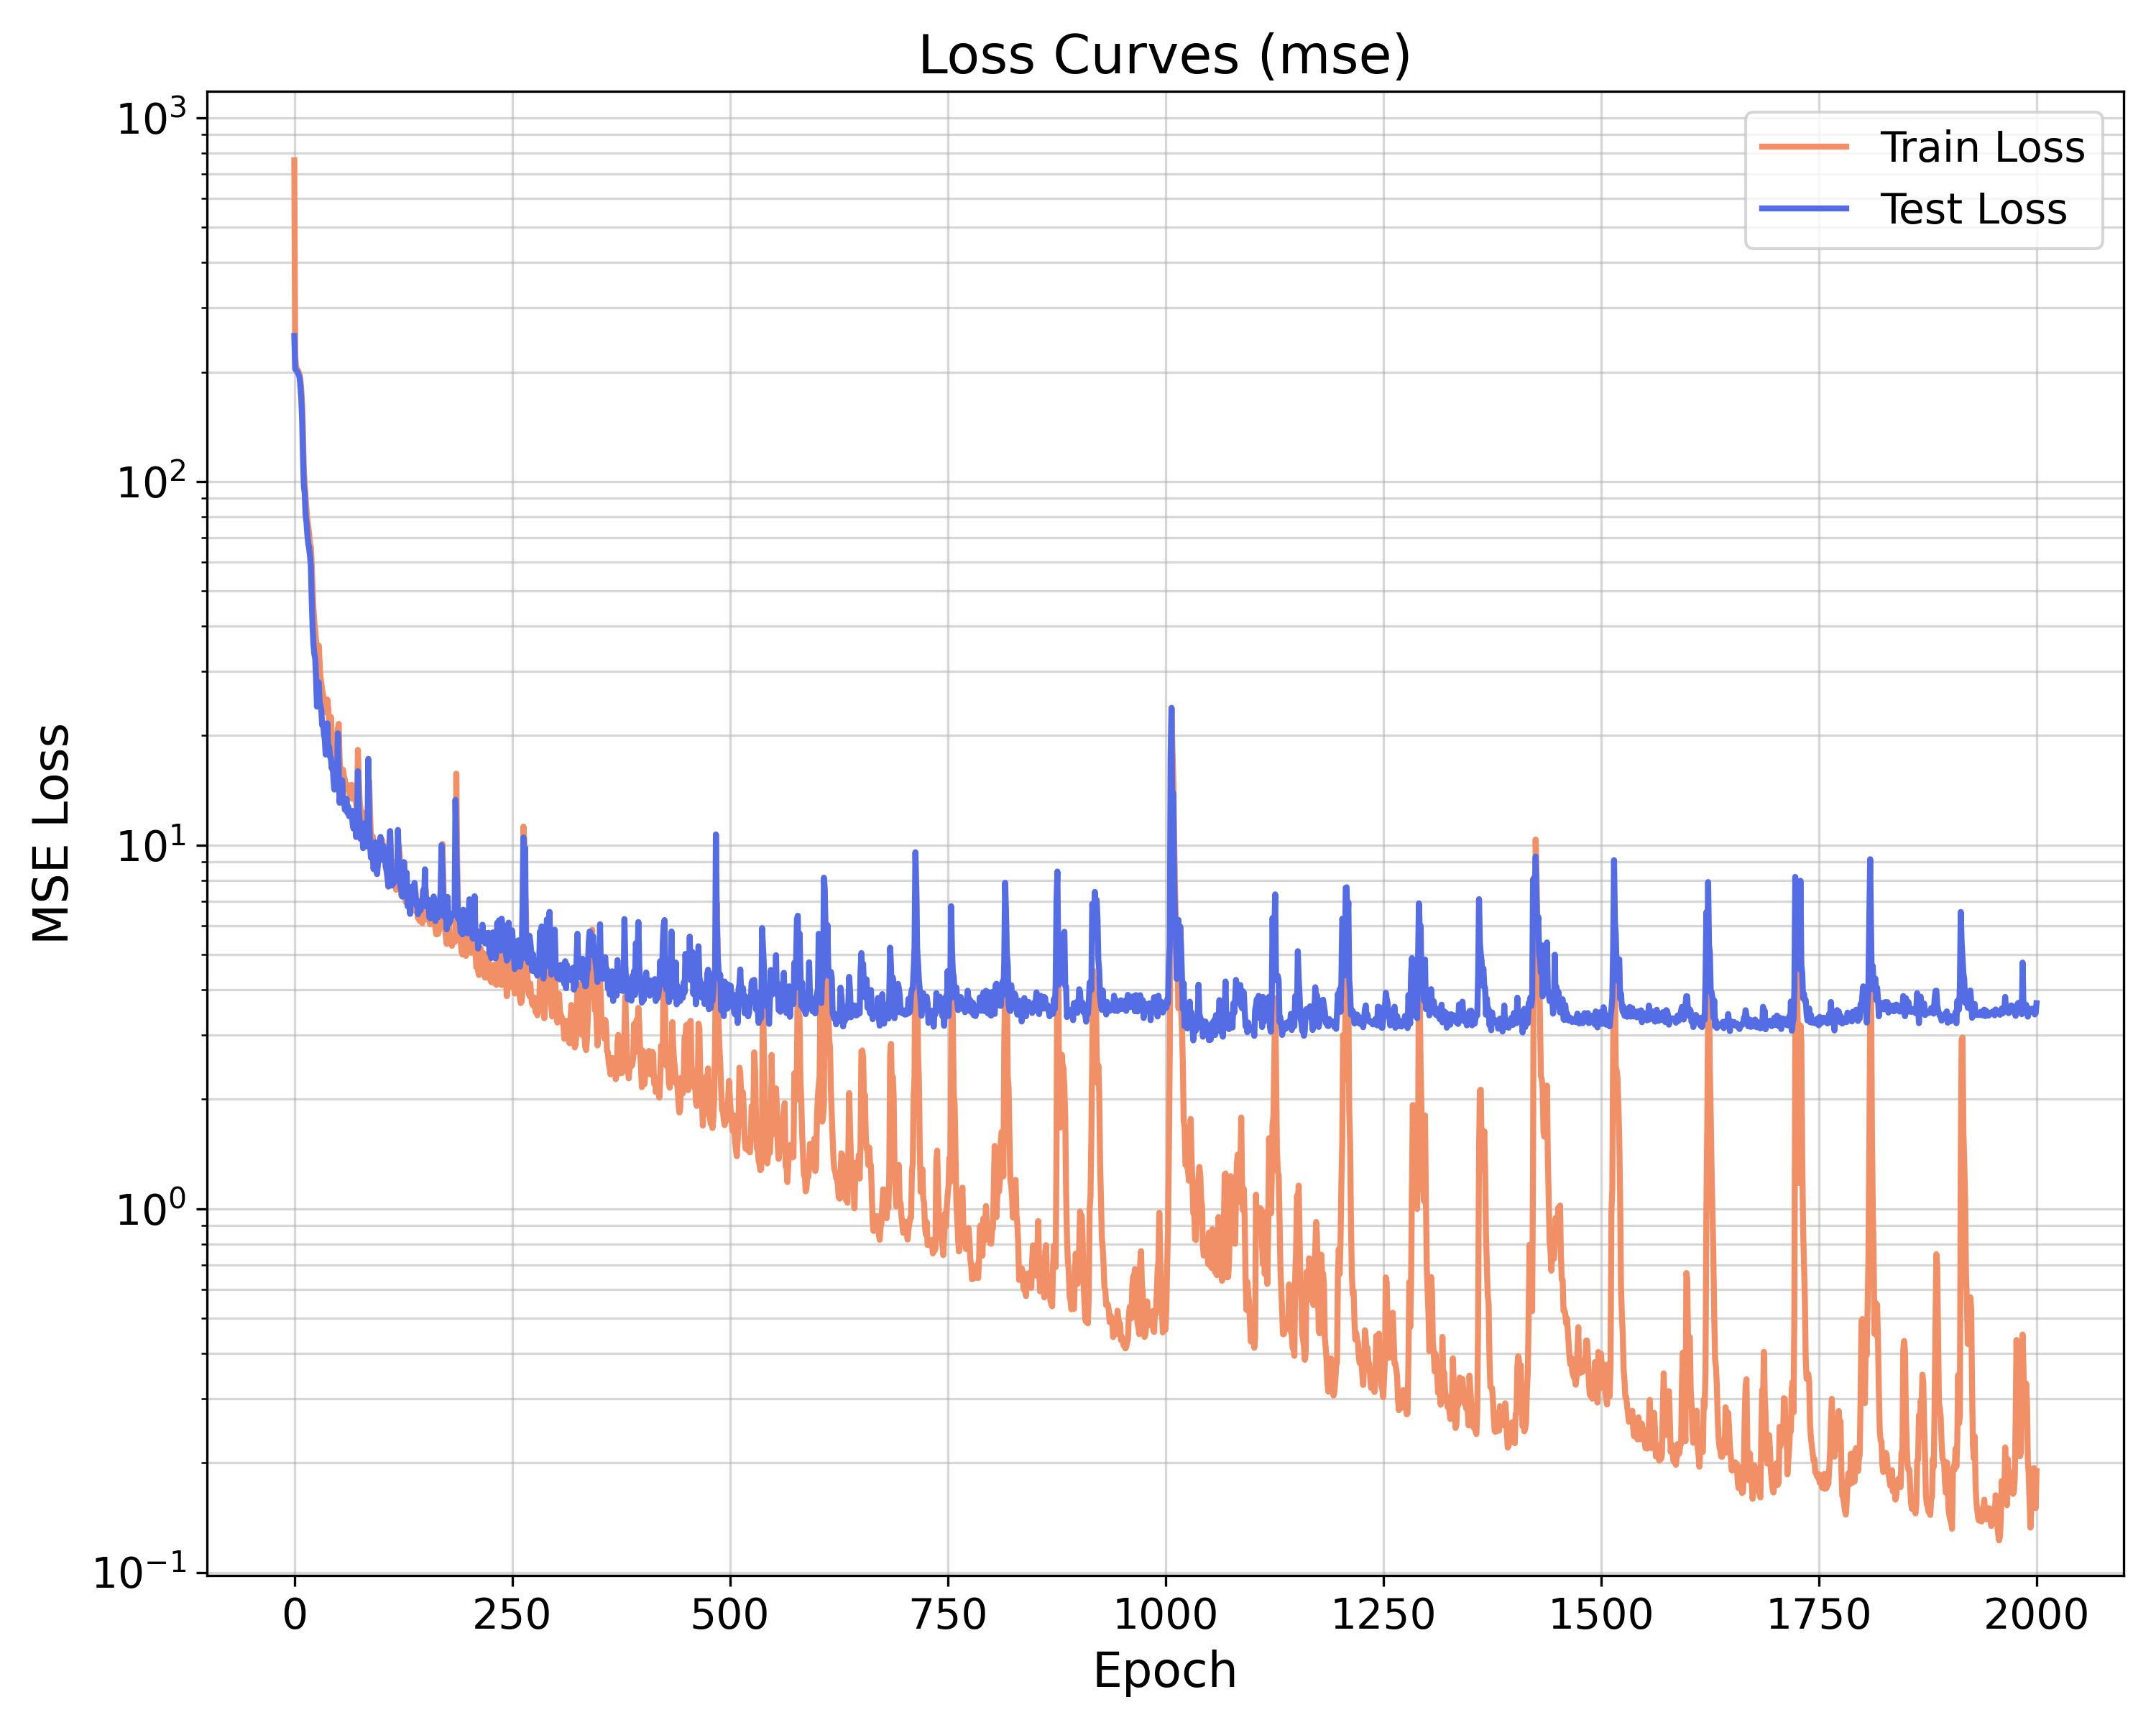
\includegraphics[width=\textwidth]{img/FH_model/BA_Network/FNO/loss_plot_fixed_S=42_N=500.png}
        \caption{$N=500$}
    \end{subfigure}
    
    \vspace{0.4cm}
    
    % --- Terza riga ---
    \begin{subfigure}[b]{0.32\textwidth}
        \centering
        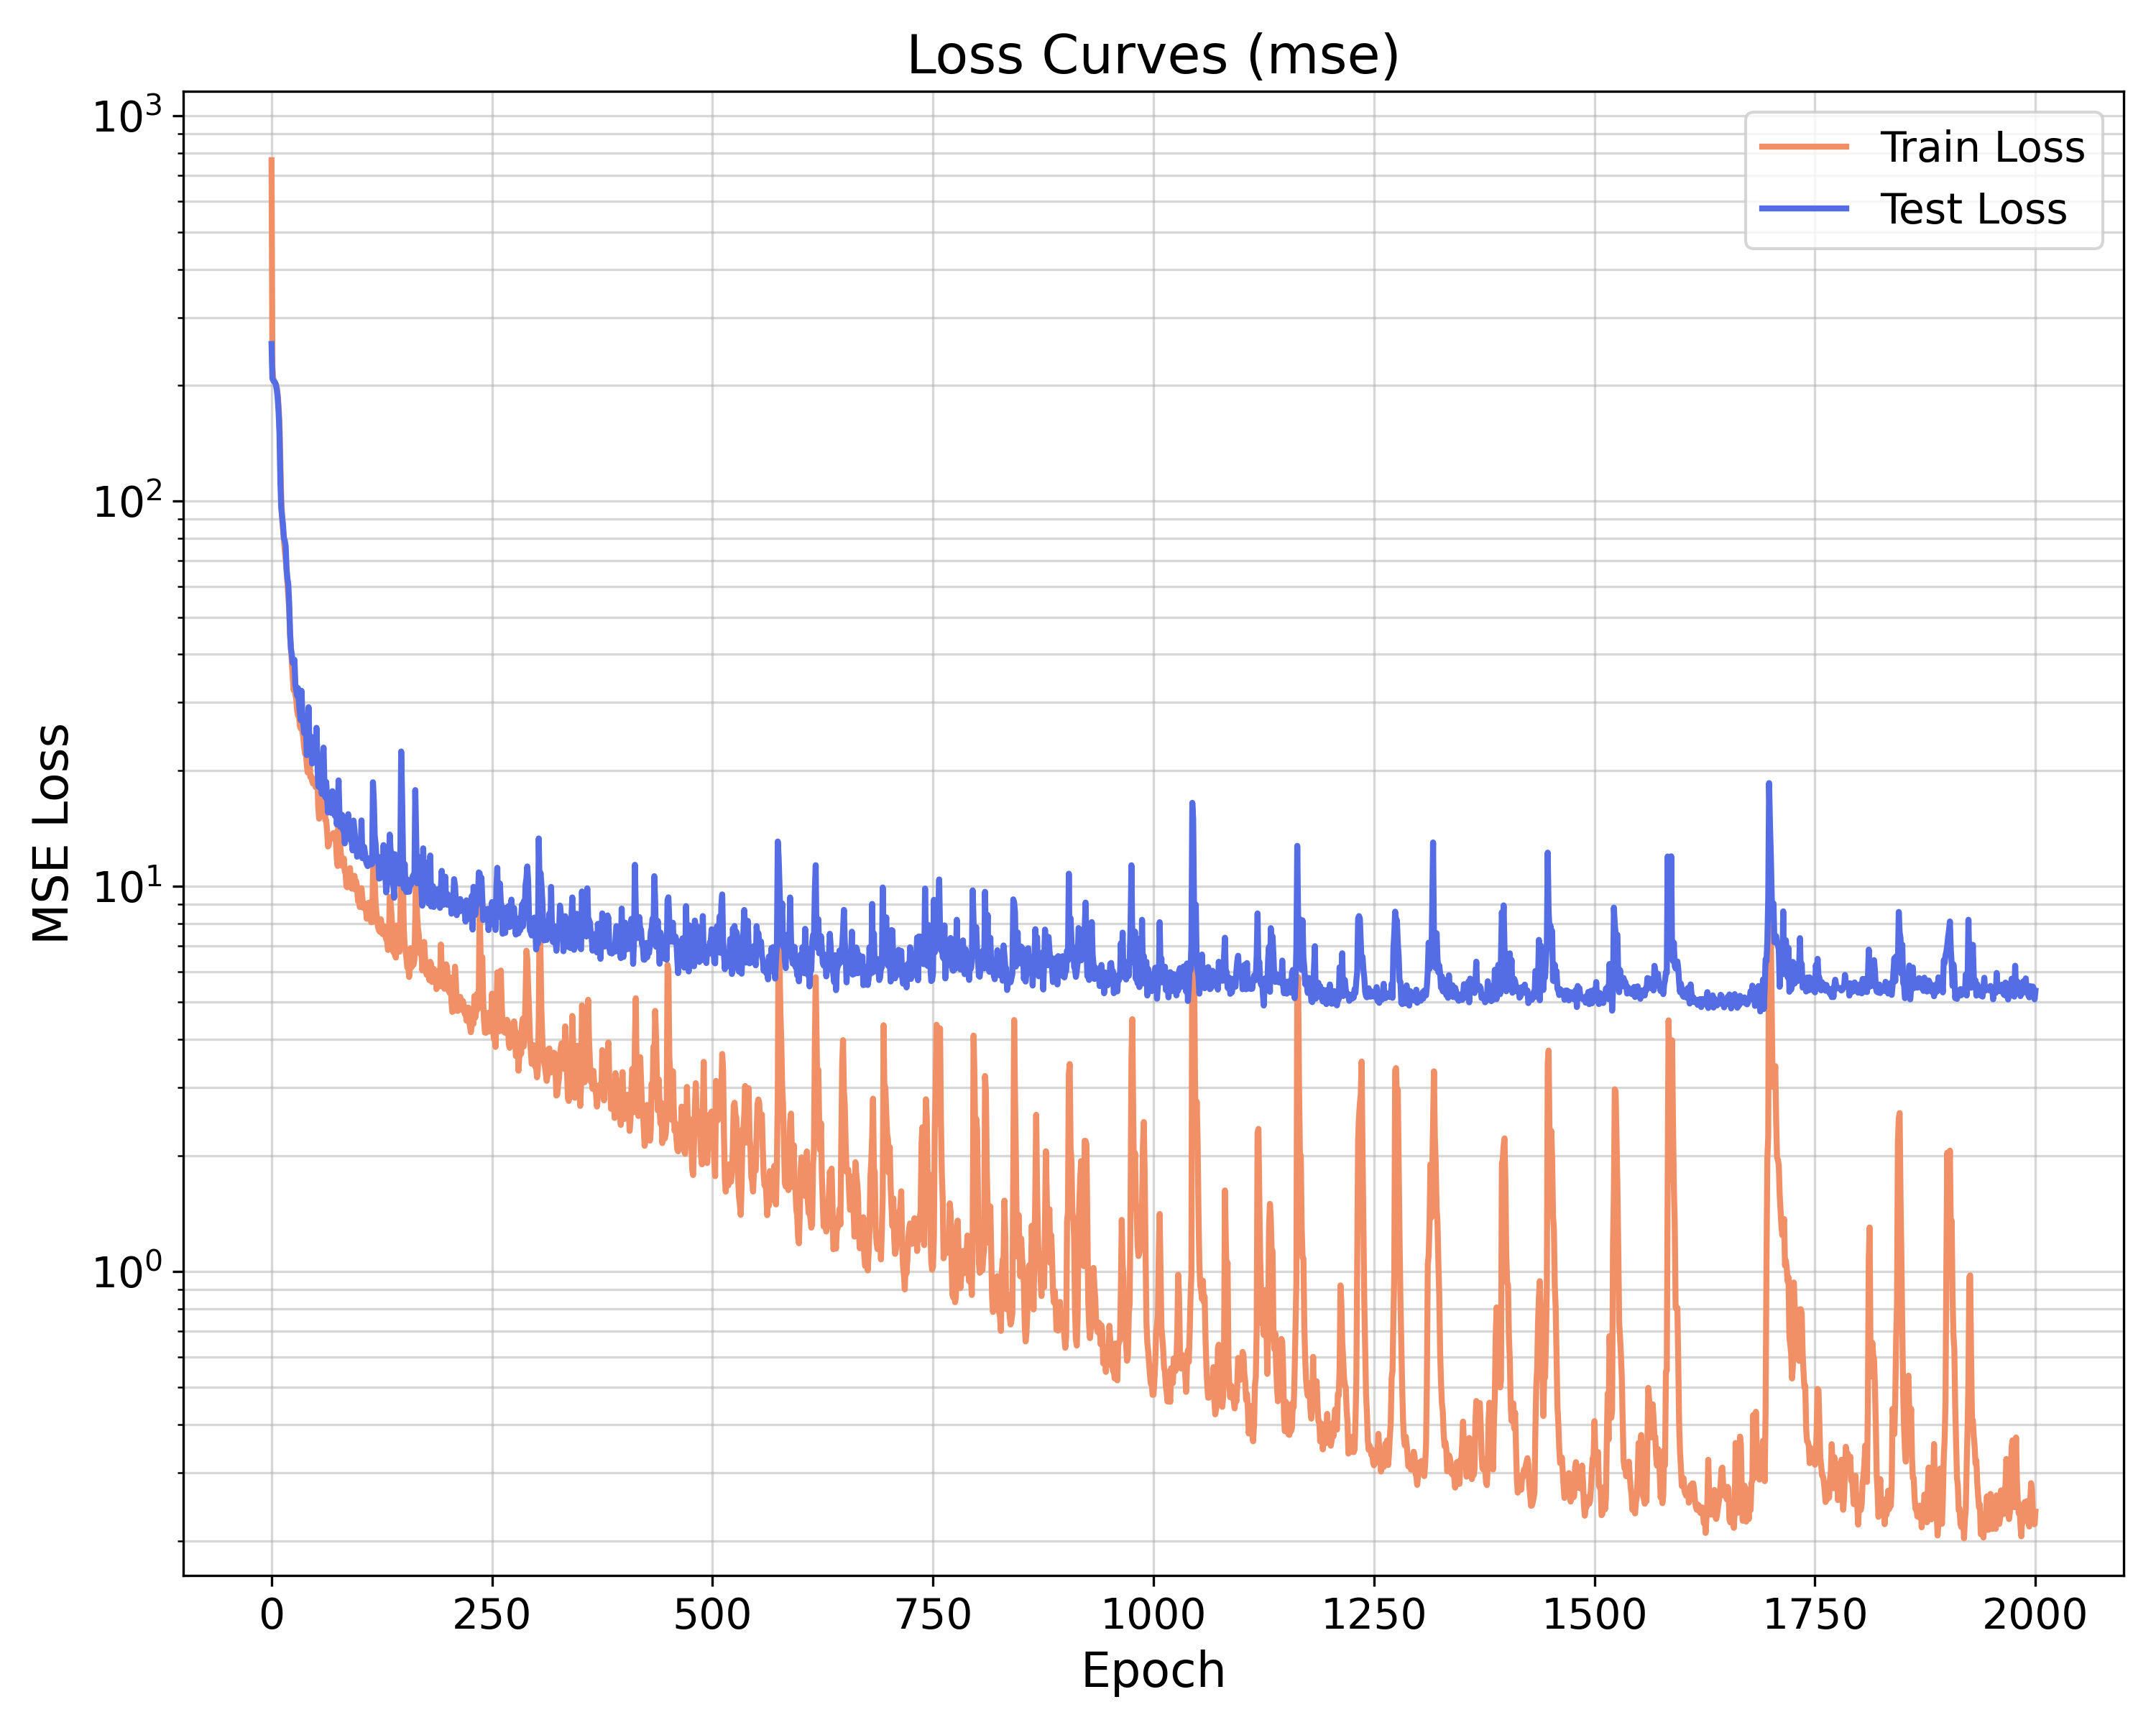
\includegraphics[width=\textwidth]{img/FH_model/BA_Network/FNO/loss_plot_fixed_S=42_N=600.png}
        \caption{$N=600$}
    \end{subfigure}
    \hfill
    \begin{subfigure}[b]{0.32\textwidth}
        \centering
        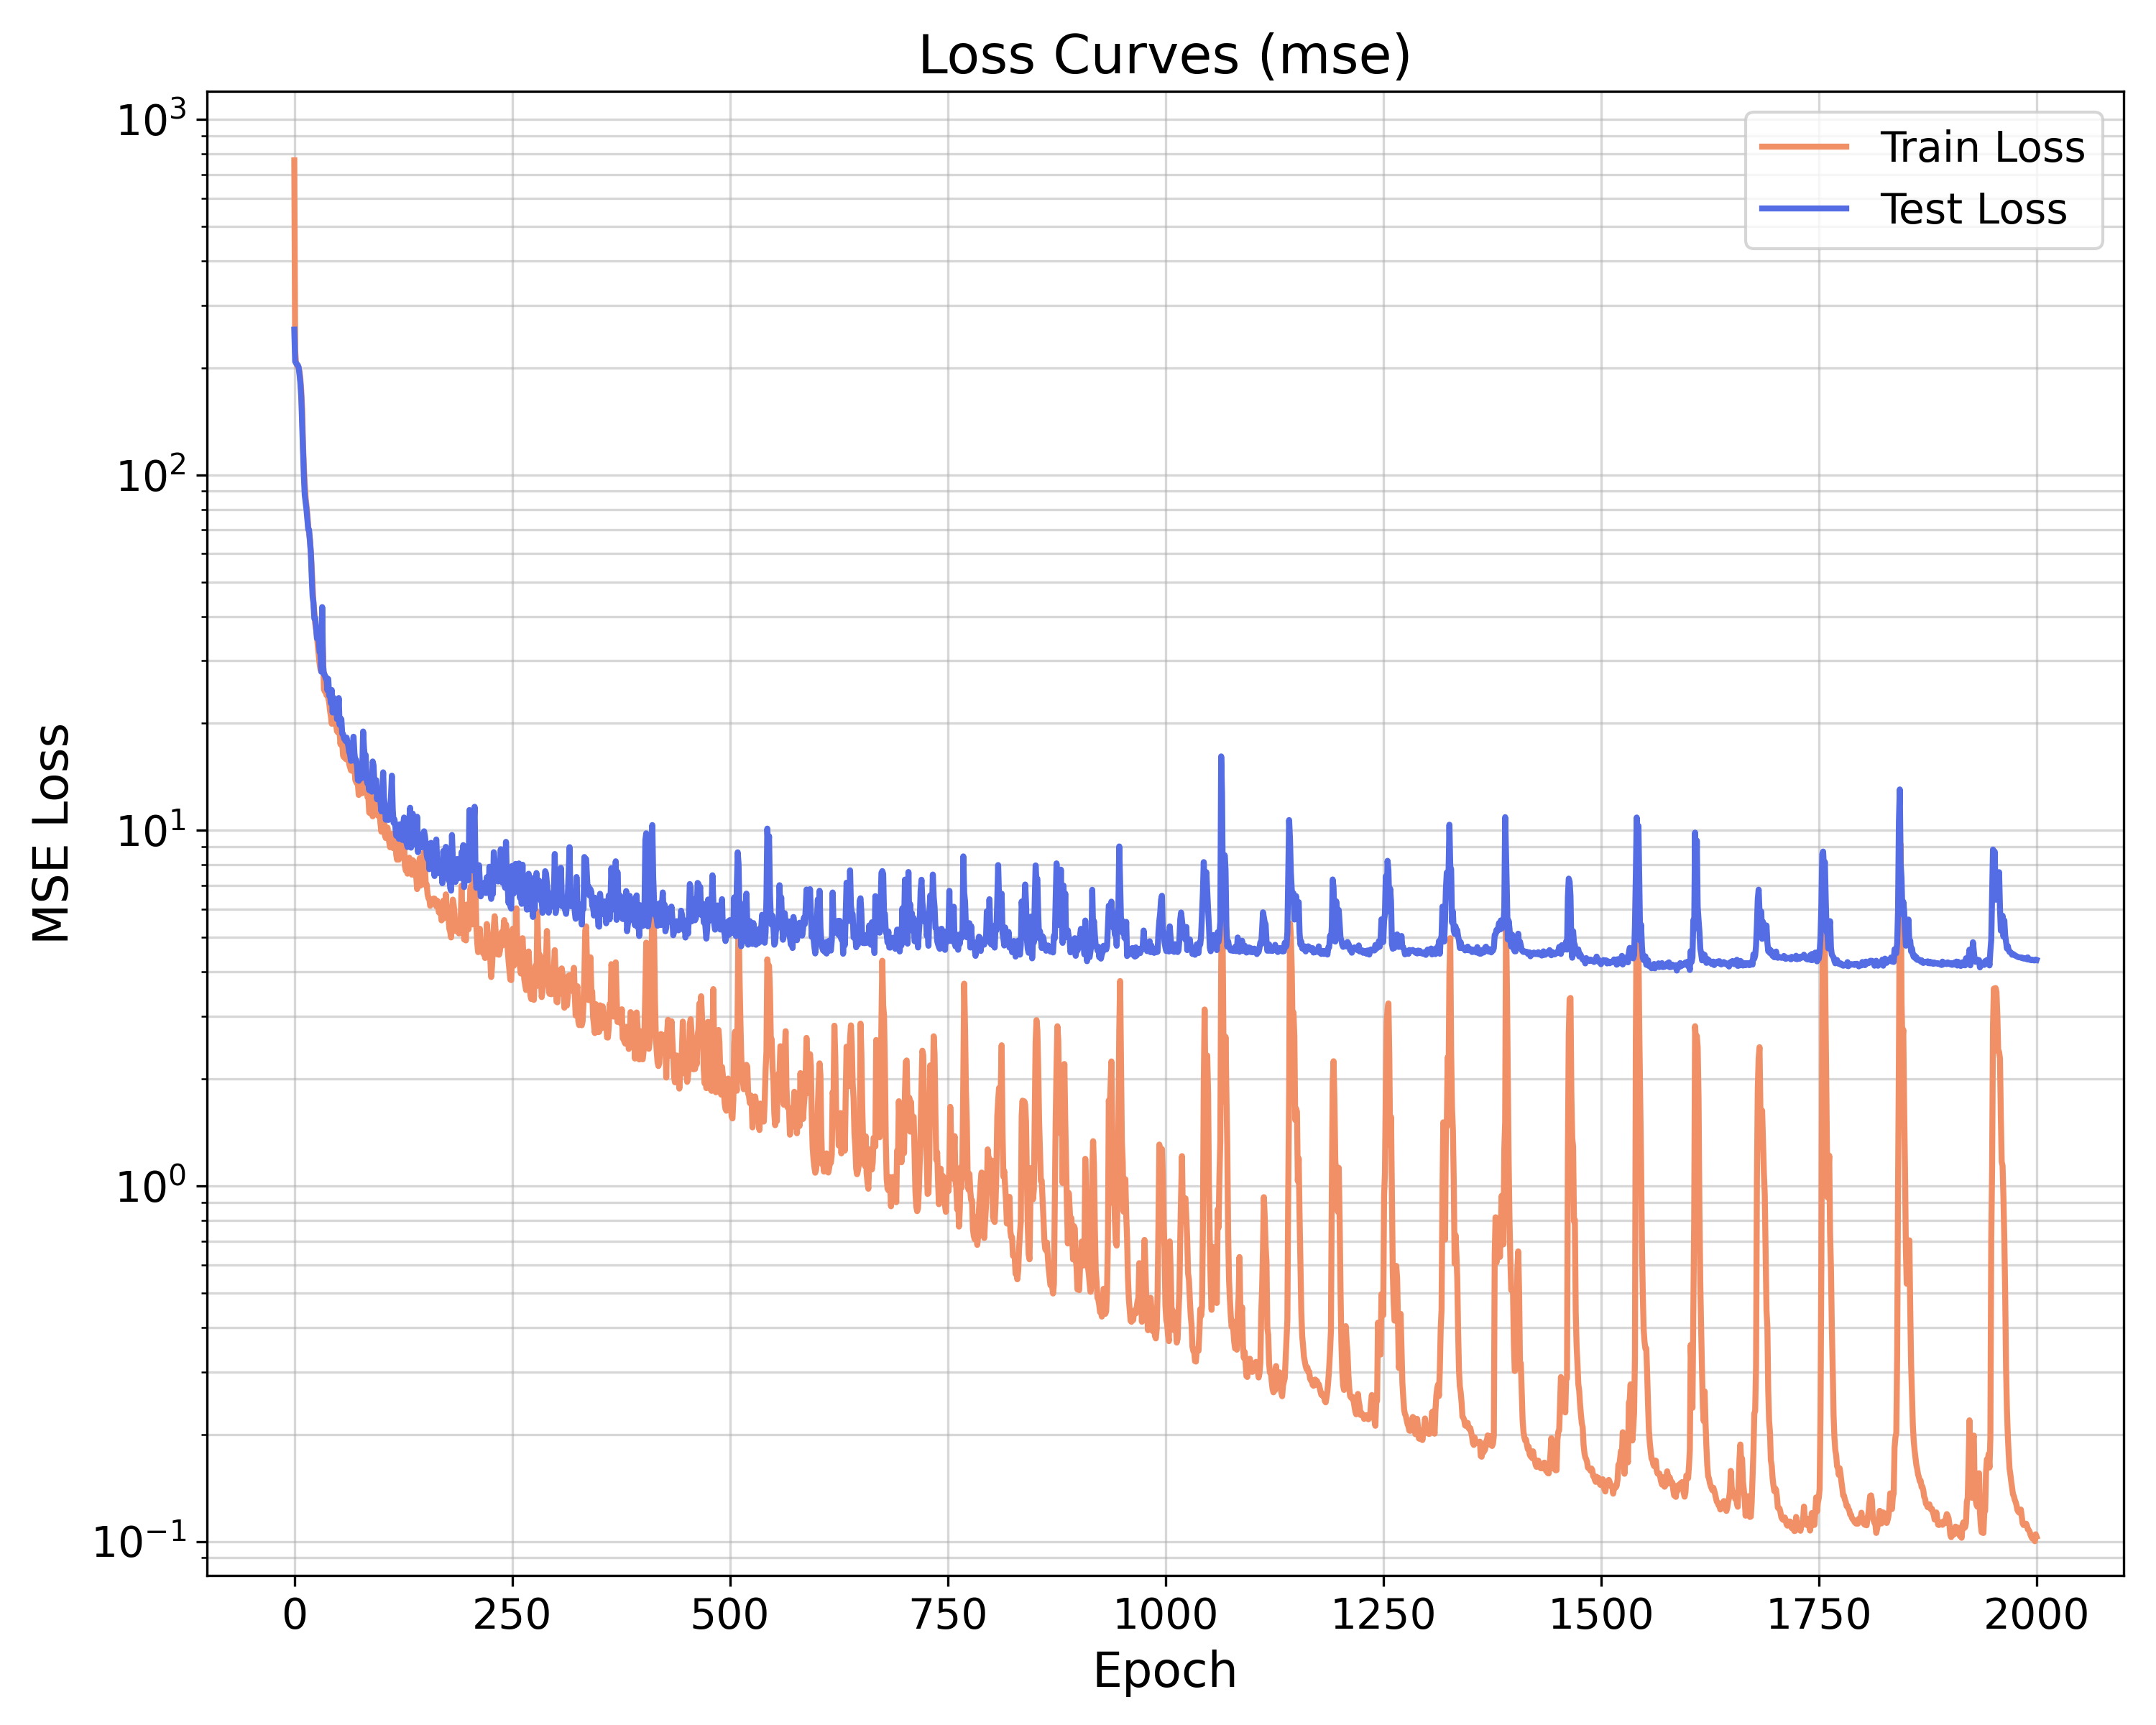
\includegraphics[width=\textwidth]{img/FH_model/BA_Network/FNO/loss_plot_fixed_S=42_N=700.png}
        \caption{$N=700$}
    \end{subfigure}
    \hfill
    \begin{subfigure}[b]{0.32\textwidth}
        \centering
        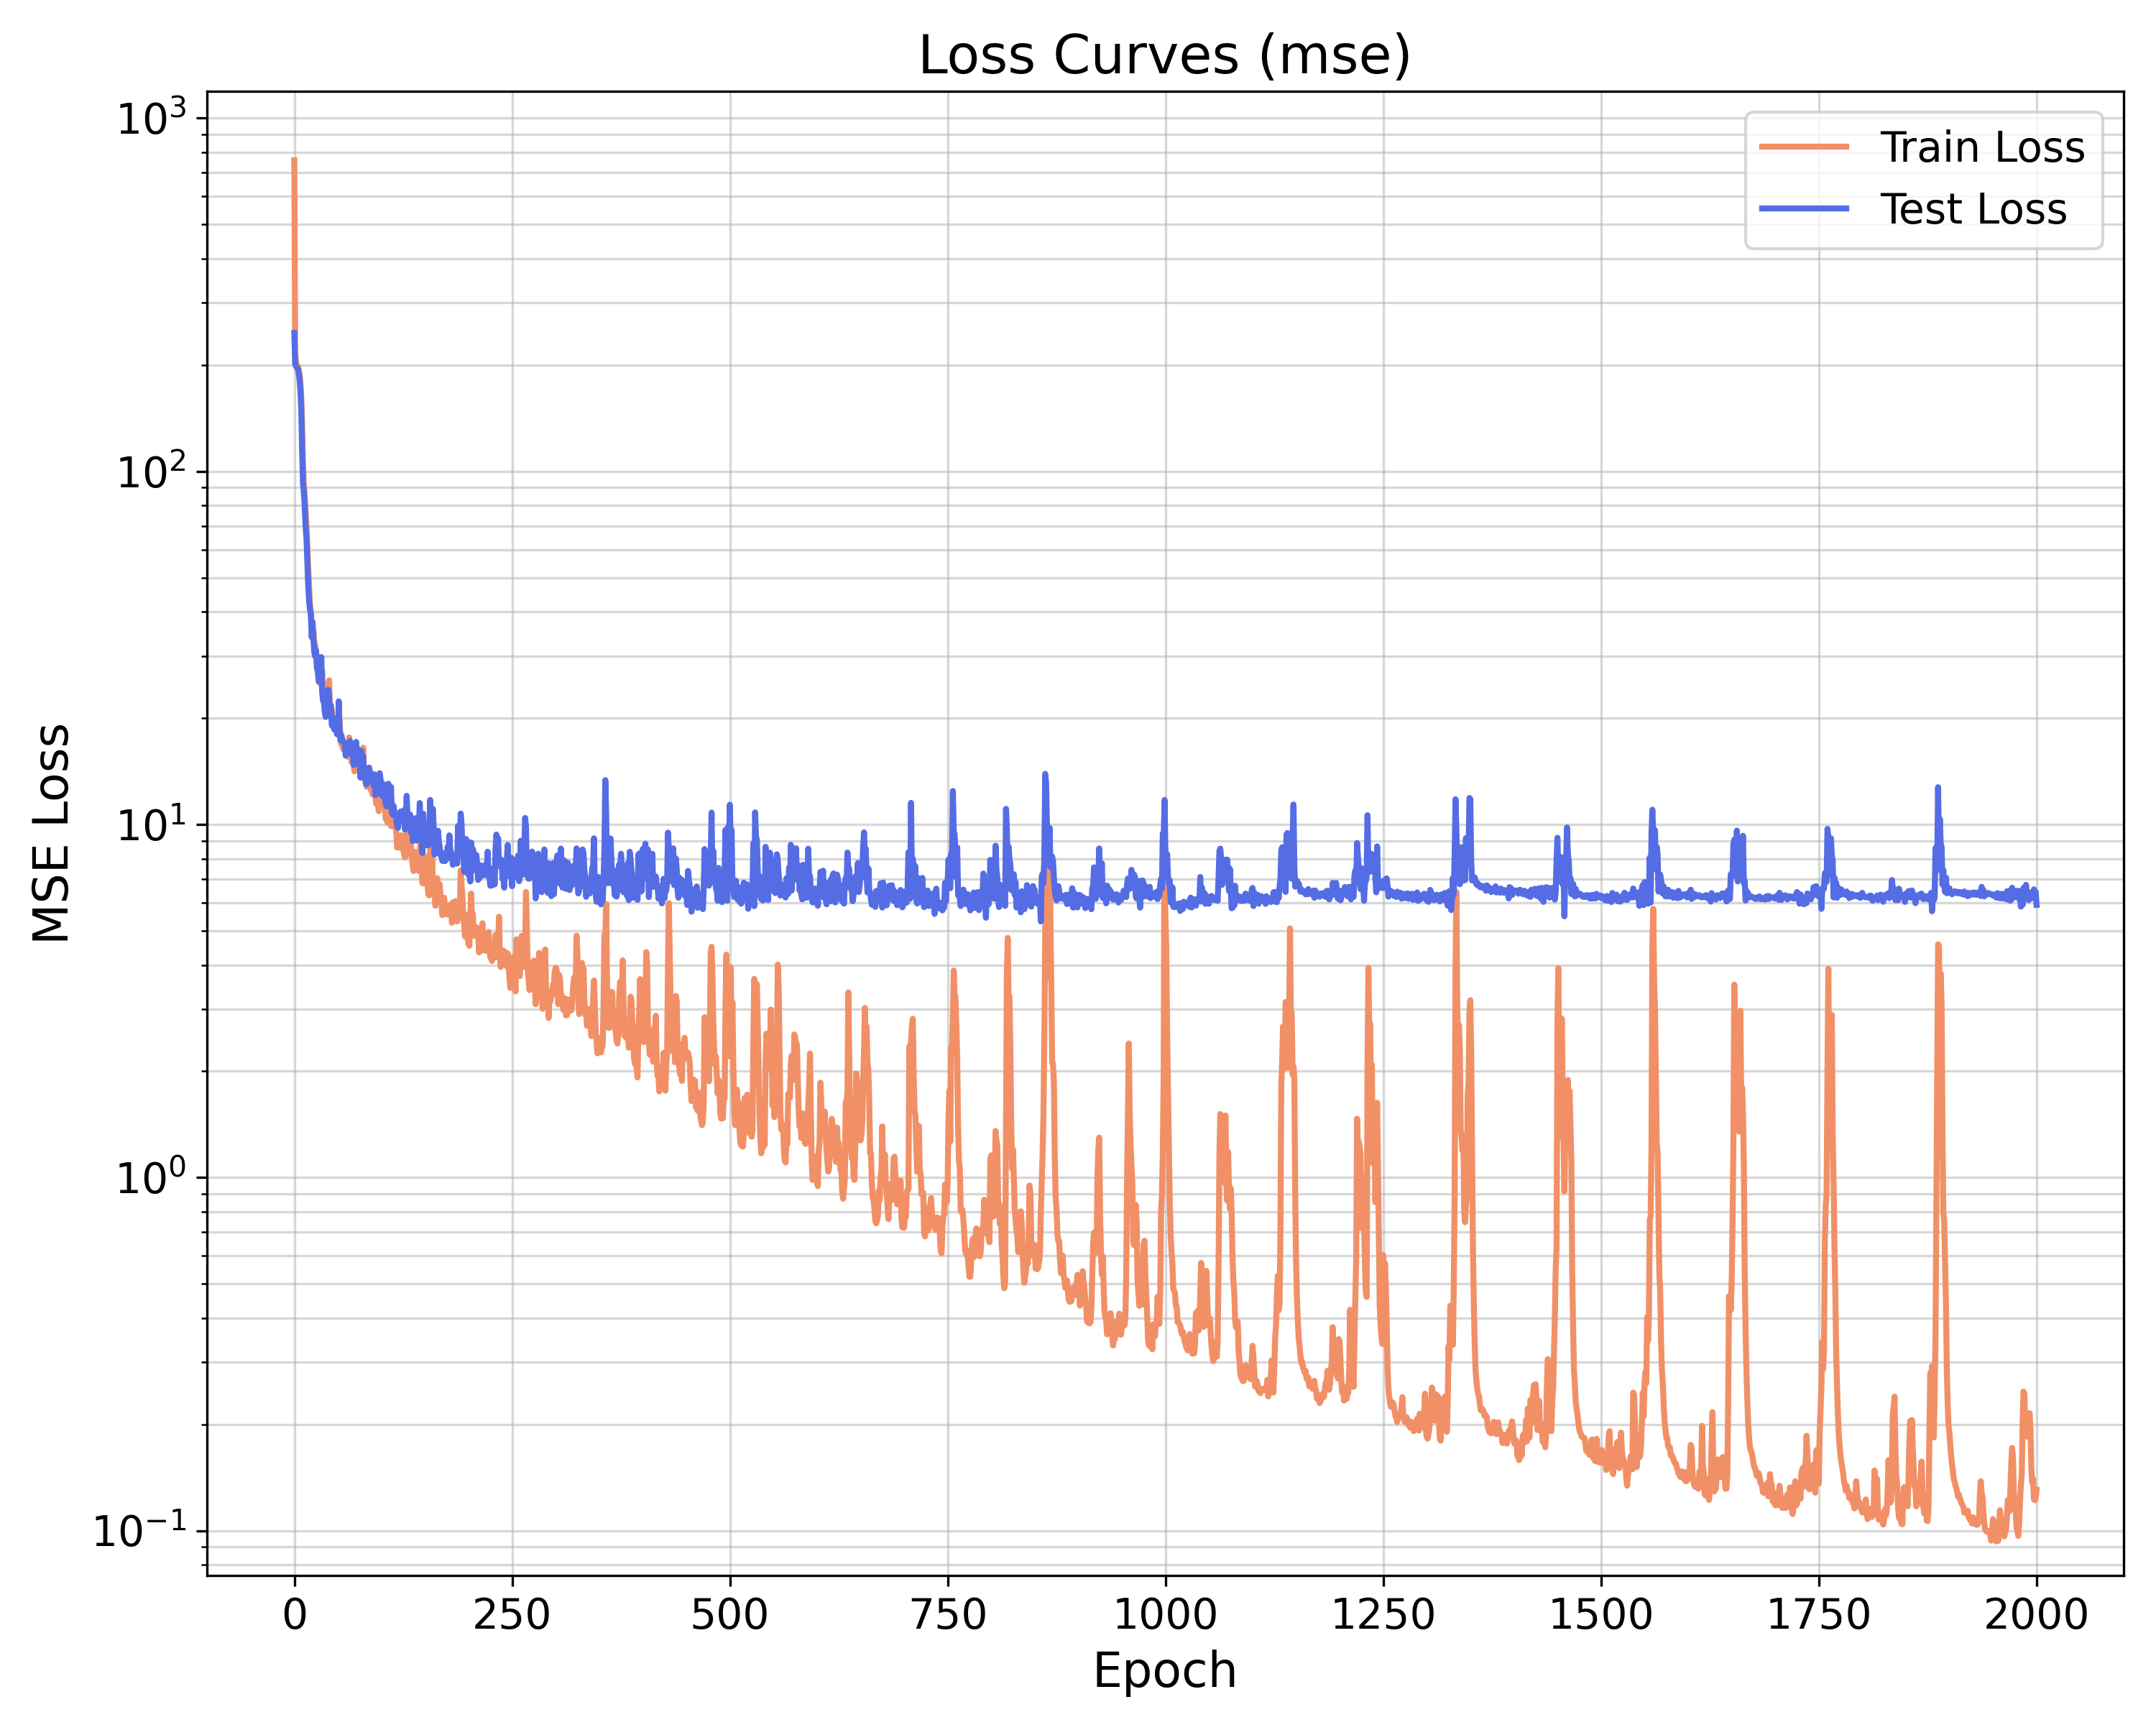
\includegraphics[width=\textwidth]{img/FH_model/BA_Network/FNO/loss_plot_fixed_S=42_N=800.png}
        \caption{$N=800$}
    \end{subfigure}
    
    \vspace{0.4cm}
    
    % --- Quarta riga ---
    \begin{subfigure}[b]{0.32\textwidth}
        \centering
        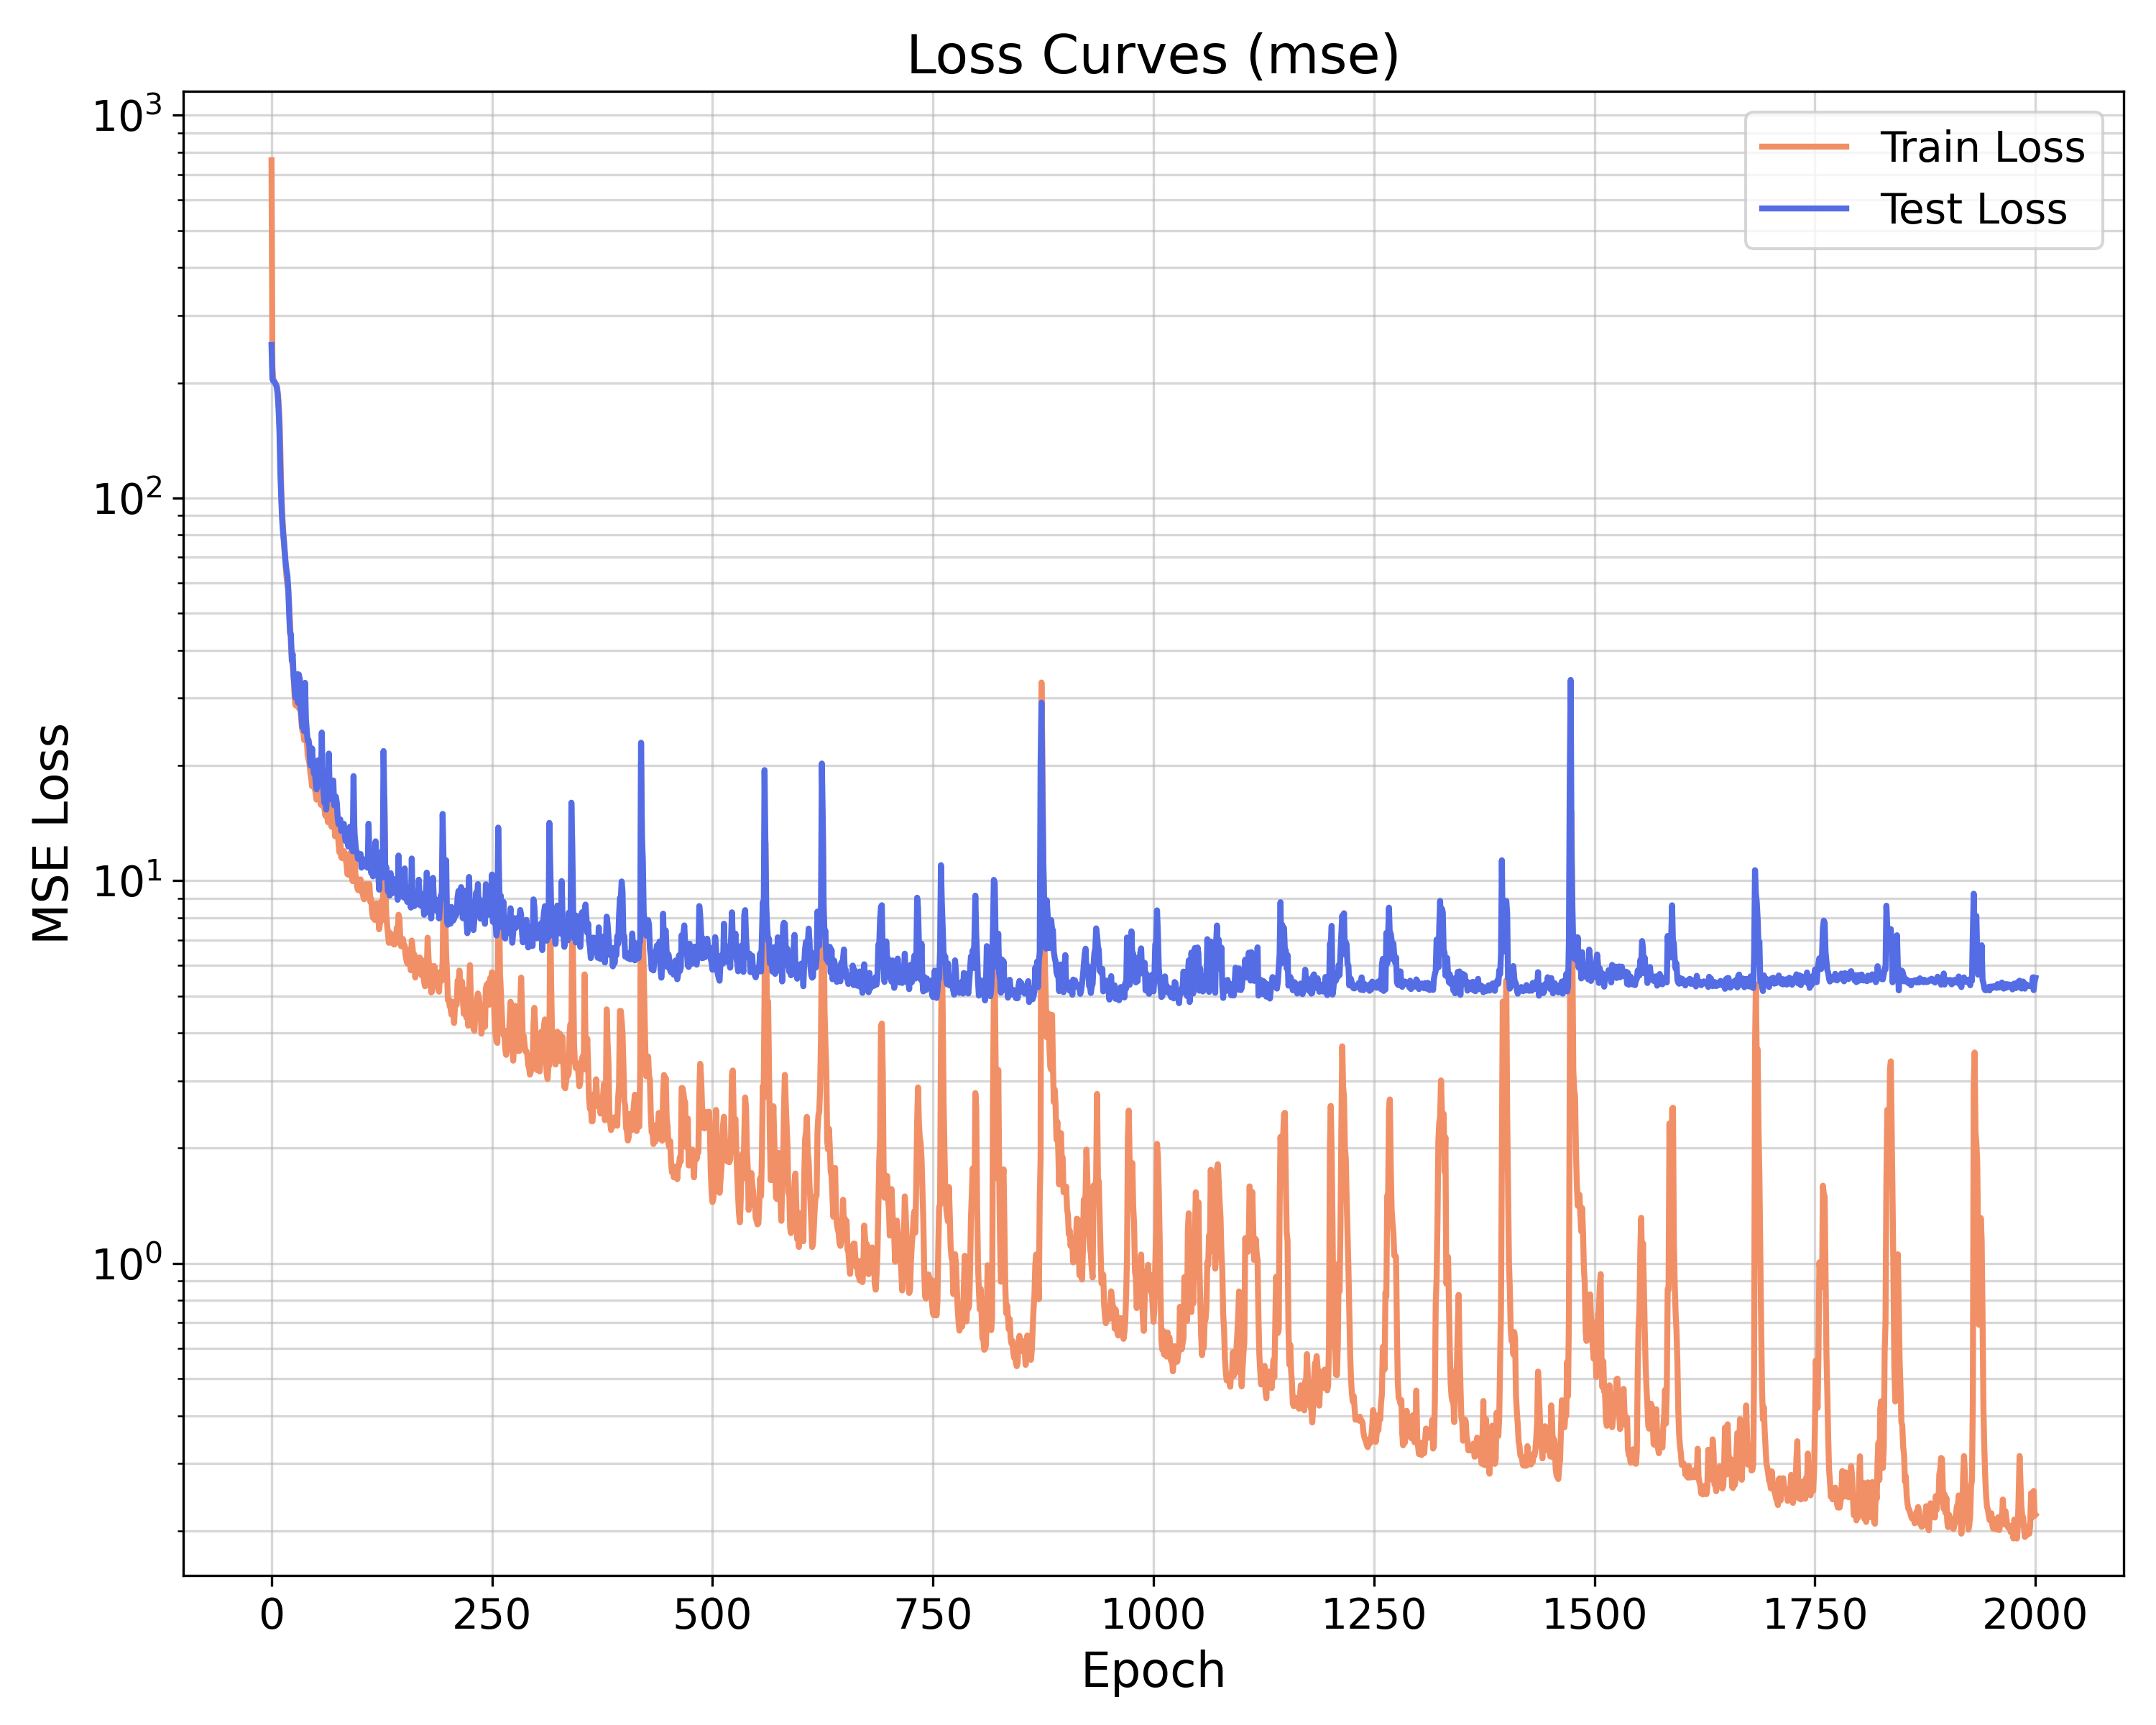
\includegraphics[width=\textwidth]{img/FH_model/BA_Network/FNO/loss_plot_fixed_S=42_N=900.png}
        \caption{$N=900$}
    \end{subfigure}
    \hfill
    \begin{subfigure}[b]{0.32\textwidth}
        \centering
        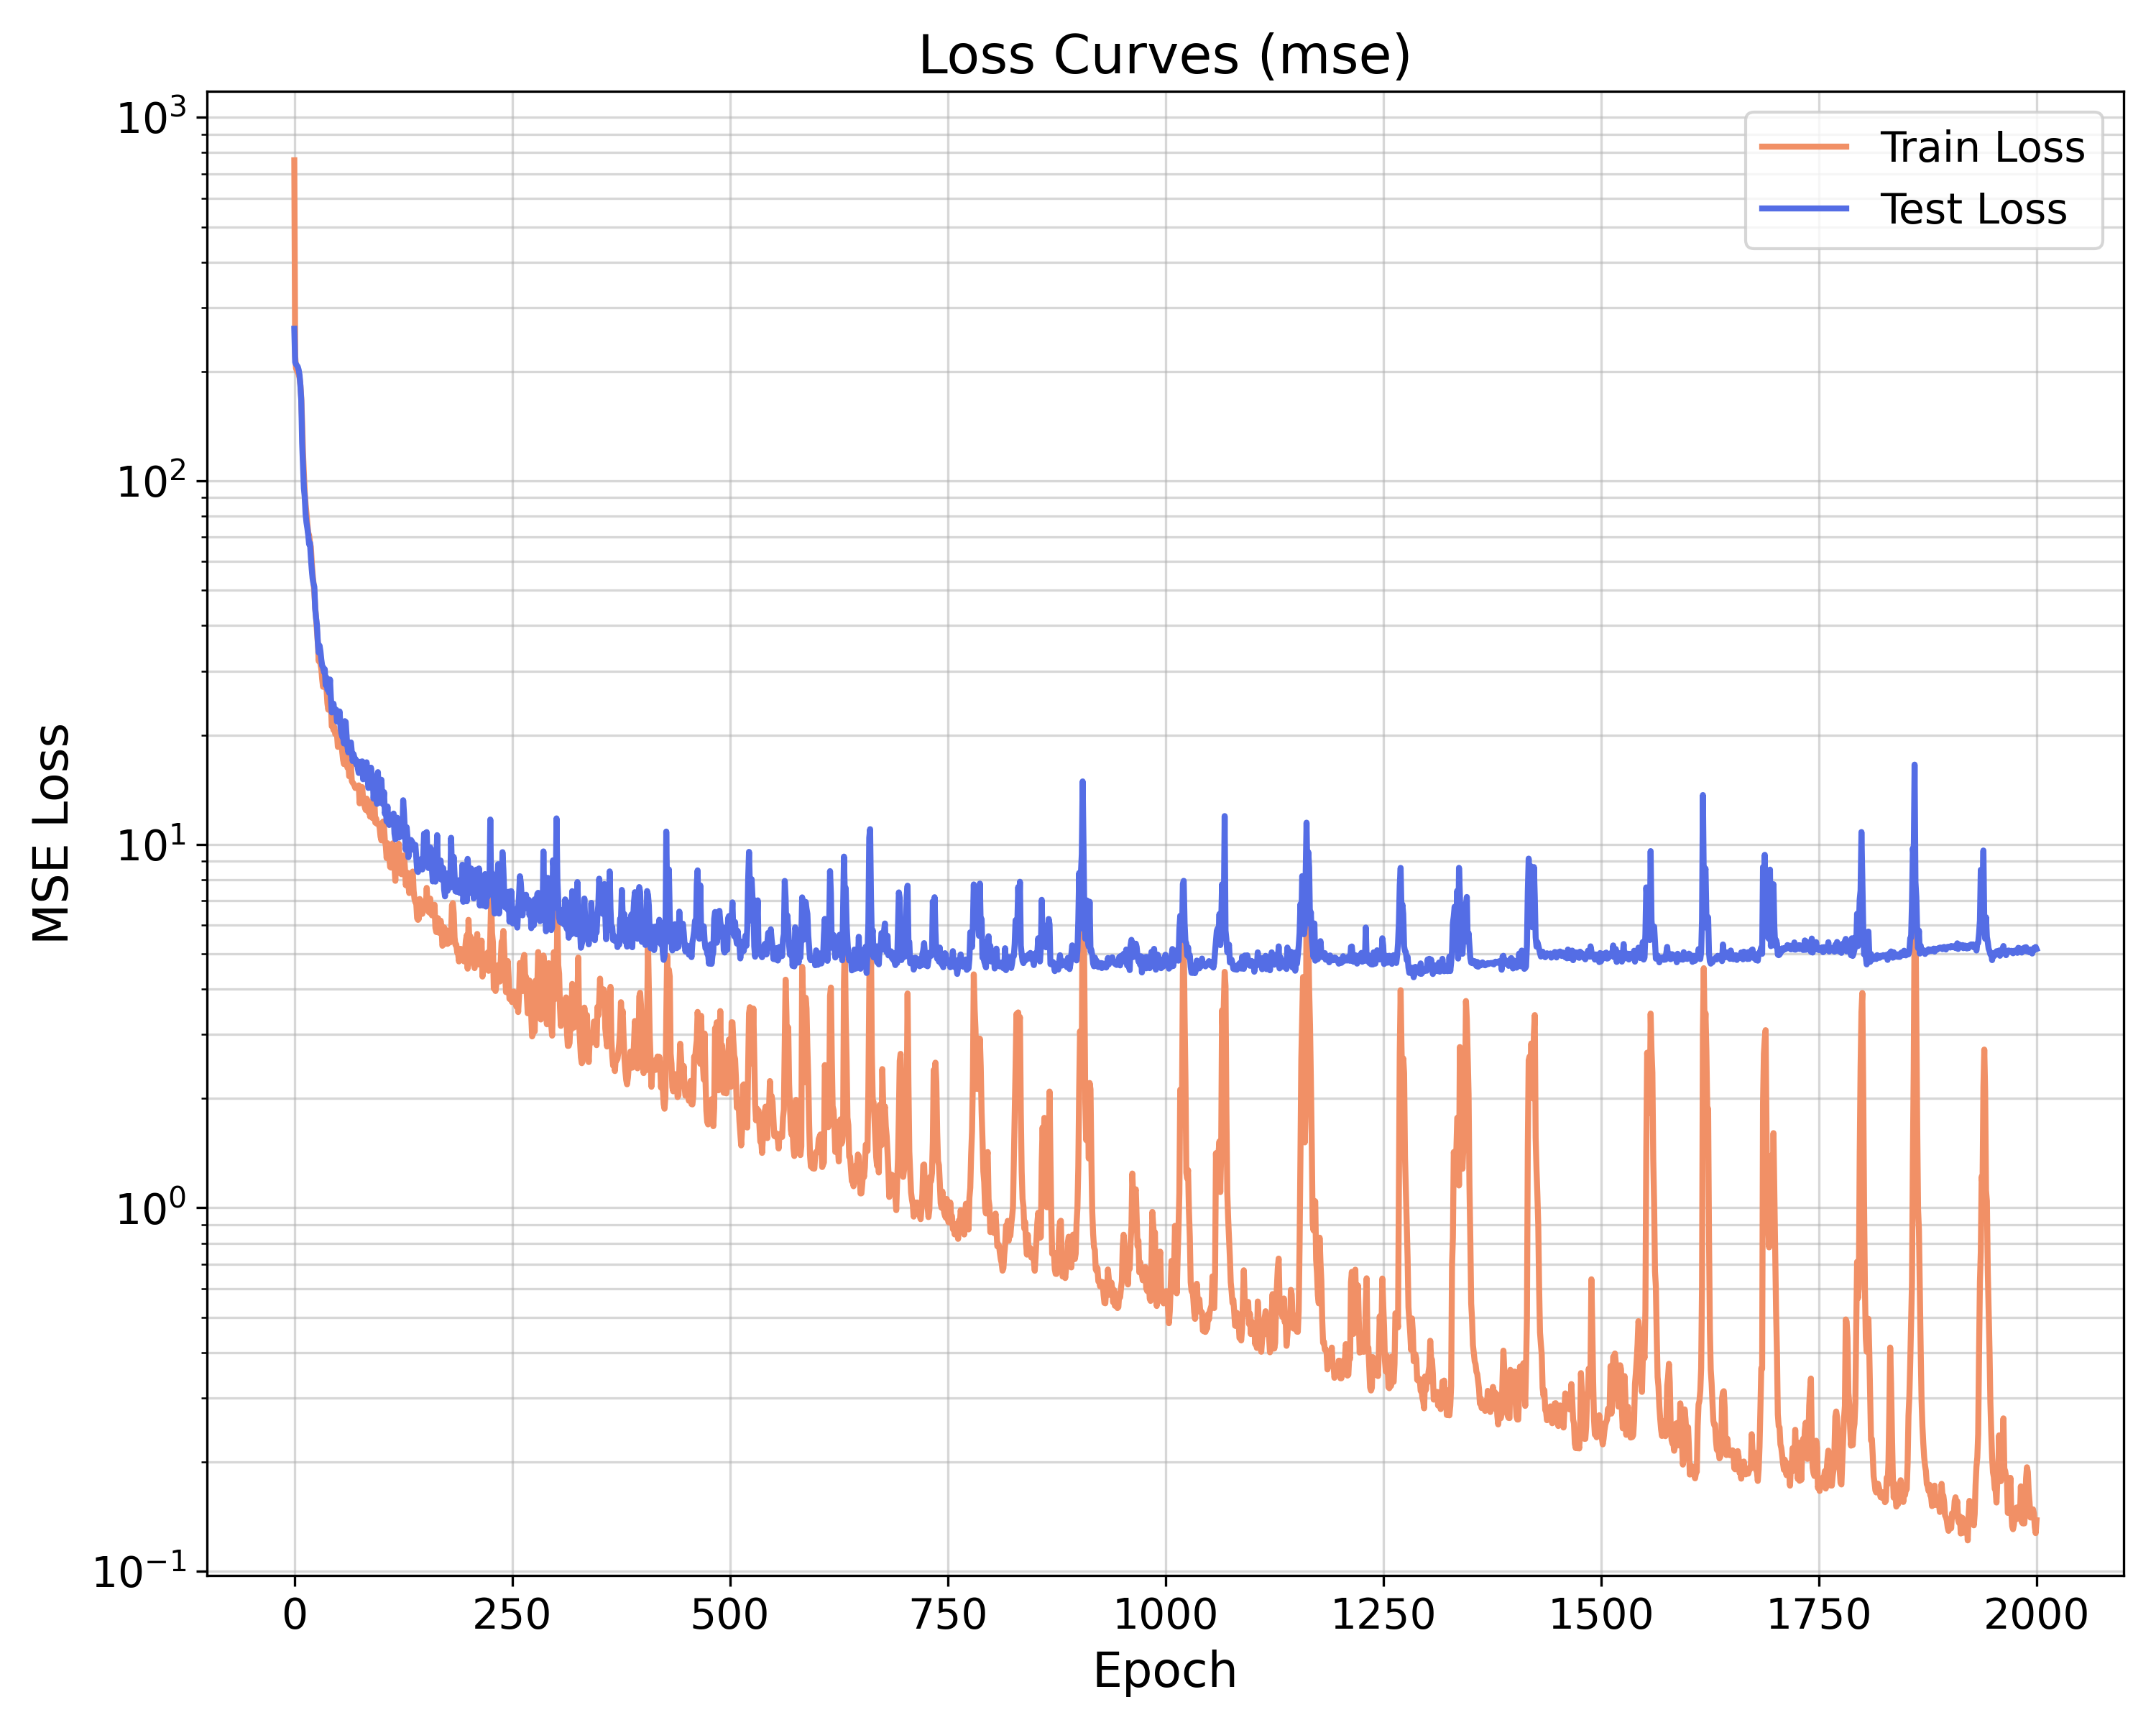
\includegraphics[width=\textwidth]{img/FH_model/BA_Network/FNO/loss_plot_fixed_S=42_N=1000.png}
        \caption{$N=1000$}
    \end{subfigure}
    \hfill
    \begin{subfigure}[b]{0.32\textwidth}
        \centering
        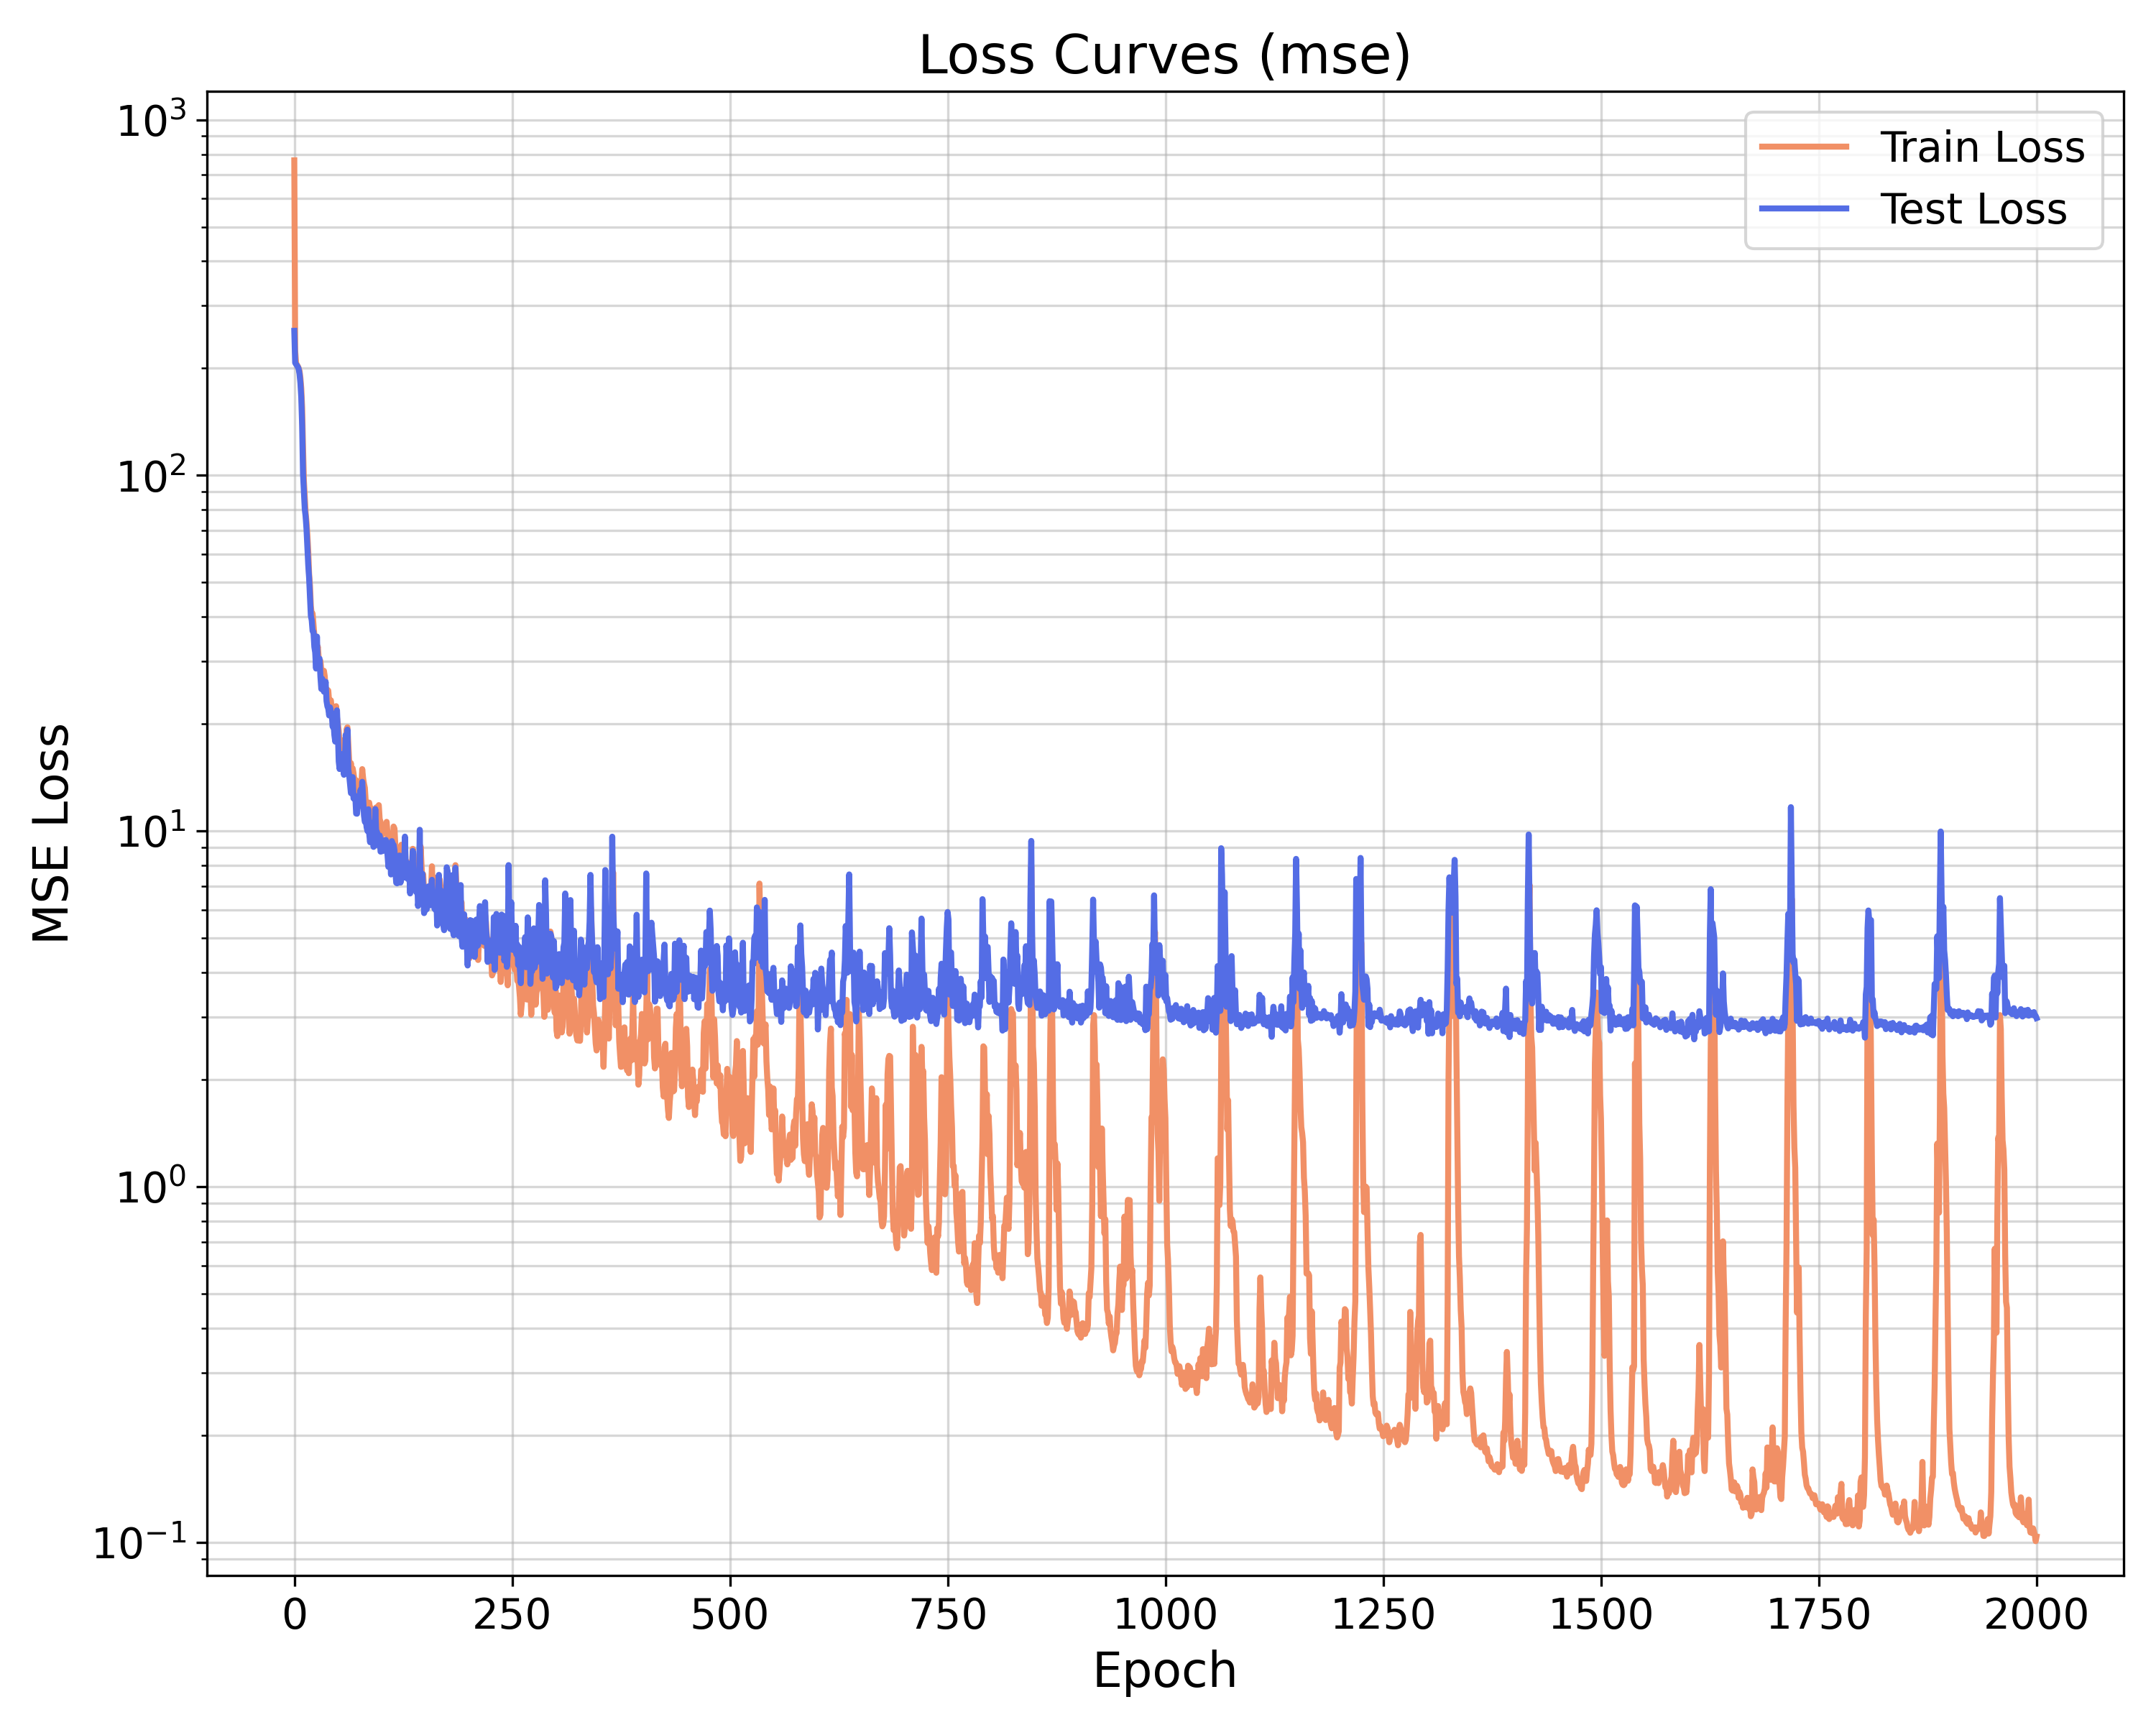
\includegraphics[width=\textwidth]{img/FH_model/BA_Network/FNO/loss_plot_fixed_S=42_N=2000.png}
        \caption{$N=2000$}
    \end{subfigure}
    
    \caption{Training and test loss convergence for different Barab\'asi-Albert network sizes ($N$).}
    \label{fig:ba_loss_grid}
\end{figure}


%% Il caso N=100 mi sembra un po' diverso dagli altri. Devo commentarlo? Forse c'è un path più breve tra input ed output.

\subsubsection{Performance across different sizes of the hidden network: Conclusion}

As we could see in the previous graphs, and in the summary Figure \ref{fig:fno_scaling_error} below, we can deduce that (at least for the sizes considered) the FNO generalizes well the deterministic dynamics. This remarkable scalability may also be due to the discretization-invariant nature of this architecture.
% In fact we performed some test where we trained on a dataset with hidden network size $N_1$ and tested on another $N_2$ and we still got good results.
A future extension could be to investigate if this good behavior persists even if noise is introduced into the system.

\begin{figure}[htbp]
    \centering
    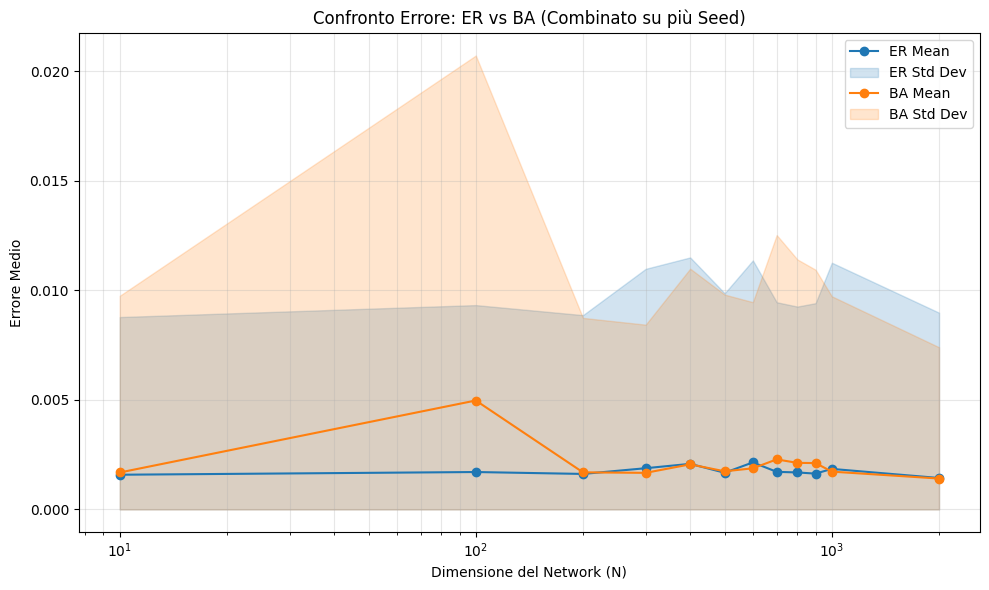
\includegraphics[width=0.8\textwidth]{img/FH_model/error_FNO_scalingN.png}
    \caption{Summary of the FNO performance across different network sizes ($N$). The plot compares the mean error scaling for both Erd\H{o}s-R\'enyi (ER) and Barab\'asi-Albert (BA) topologies, demonstrating the robustness and scalability of the architecture.}
    \label{fig:fno_scaling_error}
\end{figure}

%Test statistico?

%Collegamento con il teorema di Takens?

\subsection{C. Elegans connectonome}

\section{Dependence on the diffusion coefficient $\sigma$}

During the experiments presented in the previous sections, it became essential to understand how to appropriately tune the diffusion coefficient $\sigma$ as a function of the hidden network size $N$. In fact, if we maintain $\sigma$ fixed while $N$ increases, the transmitted energy dissipates and the output signal progressively attenuates until it completely dies out (a phenomenon akin to dynamical quenching). An initial numerical investigation suggested that the correct scaling to preserve the macroscopic dynamical regime is $\sigma = \mathcal{O}(N)$.

% Anche qui mi sa che dovrei rigenerare il grafico con le label in inglese
\begin{figure}[htbp]
    \centering
    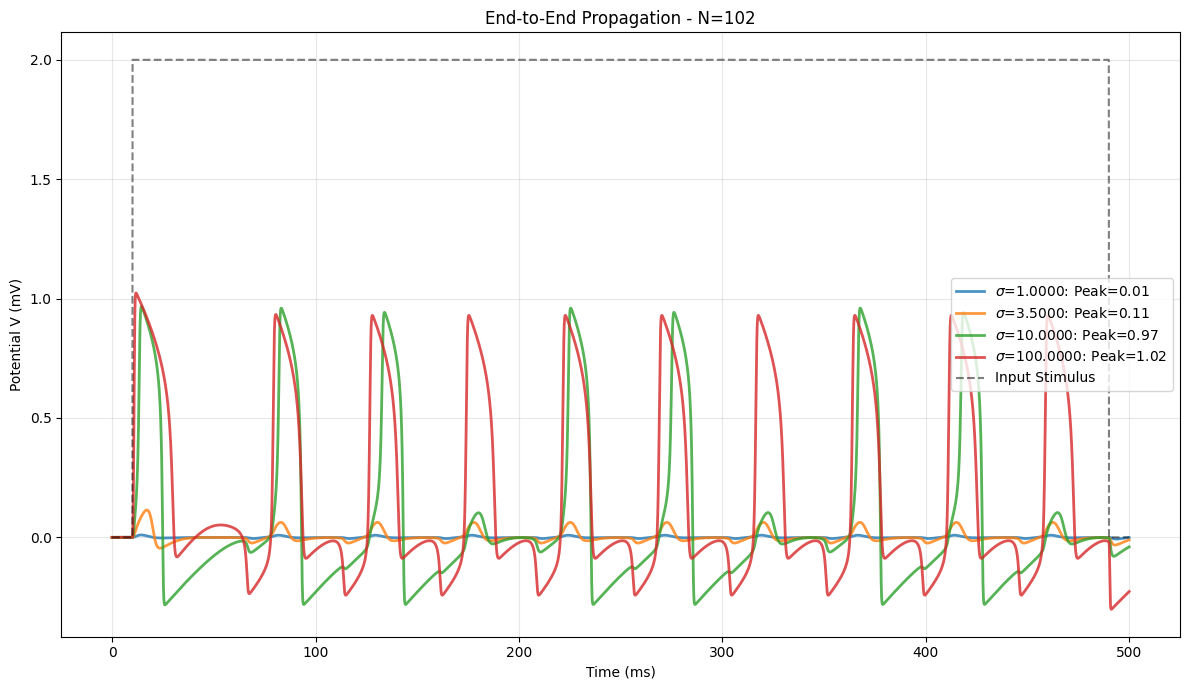
\includegraphics[width=0.8\textwidth]{img/FH_model/BA_Network/diffusion_coeff_BA_N=100.png}
    \caption{Dynamical transition of the neural network as the diffusion coefficient $\sigma$ varies. For low values of $\sigma$, the signal fails to propagate efficiently, whereas a critical threshold allows for coherent signal transmission.}
    \label{fig:diffusion_transition}
\end{figure}

%Dovrei studiare qual è la critical treshold per cui il segnale passa?

This empirical observation is rigorously supported by the numerical study of the spectral gap of the network's directed Laplacian, specifically the first non-zero real part of the eigenvalues, $\text{Re}(\lambda_2)$. In networked dynamical systems, the global synchronization and the ability of a perturbation to travel across the graph without quenching are governed by the effective macroscopic diffusion rate, which is proportional to the product $\sigma \text{Re}(\lambda_2)$ \cite{barrat2008dynamical}. 

Although standard Erdős–Rényi (ER) and Barabási-Albert (BA) graphs typically exhibit a spectral gap that decays logarithmically as $\mathcal{O}((\ln N)^{-1})$ due to their small-world properties, the strict structural bottleneck introduced by our specific boundary conditions (forcing the flow through a single input node and a single output node) profoundly alters the transport topology. This boundary constraint effectively forces the energy flow into a quasi-one-dimensional transport regime. As a result, our numerical spectral analysis demonstrates that $\text{Re}(\lambda_2)$ collapses linearly, scaling exactly as $\mathcal{O}(N^{-1})$ for both the ER and BA setups.

\begin{figure}[htbp]
    \centering
    \begin{minipage}{0.49\textwidth}
        \centering
        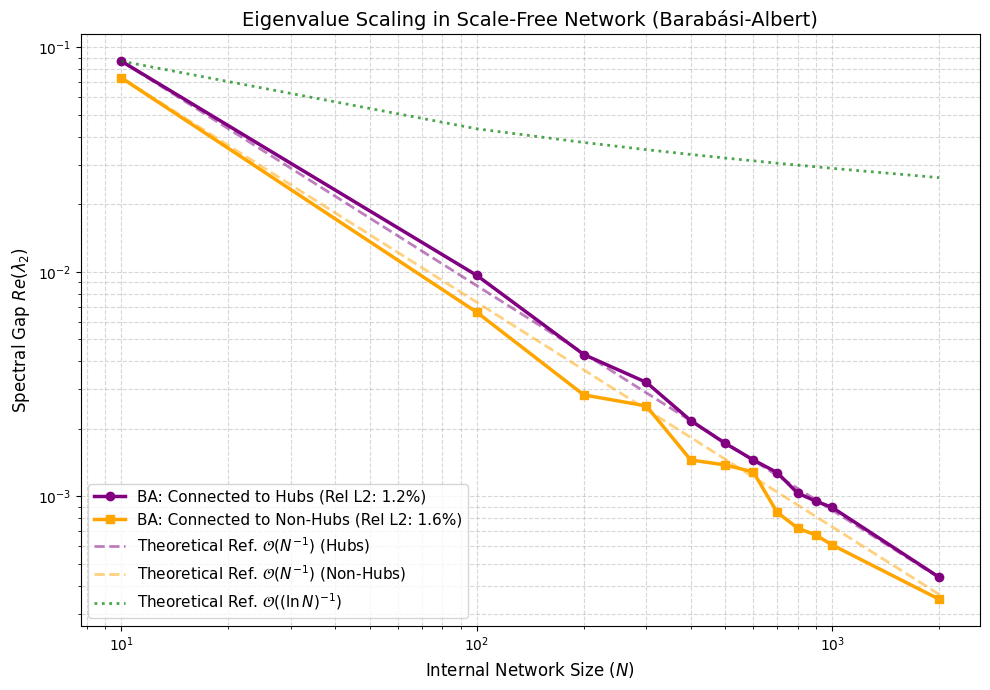
\includegraphics[width=\textwidth]{img/FH_model/BA_Network/Spectral_gap_BA.png}
        \caption{Scaling of the spectral gap $\text{Re}(\lambda_2)$ as a function of $N$ for the Barabási-Albert (BA) topology, showing the $\mathcal{O}(N^{-1})$ decay.}
        \label{fig:spectral_gap_ba}
    \end{minipage}\hfill
    \begin{minipage}{0.49\textwidth}
        \centering
        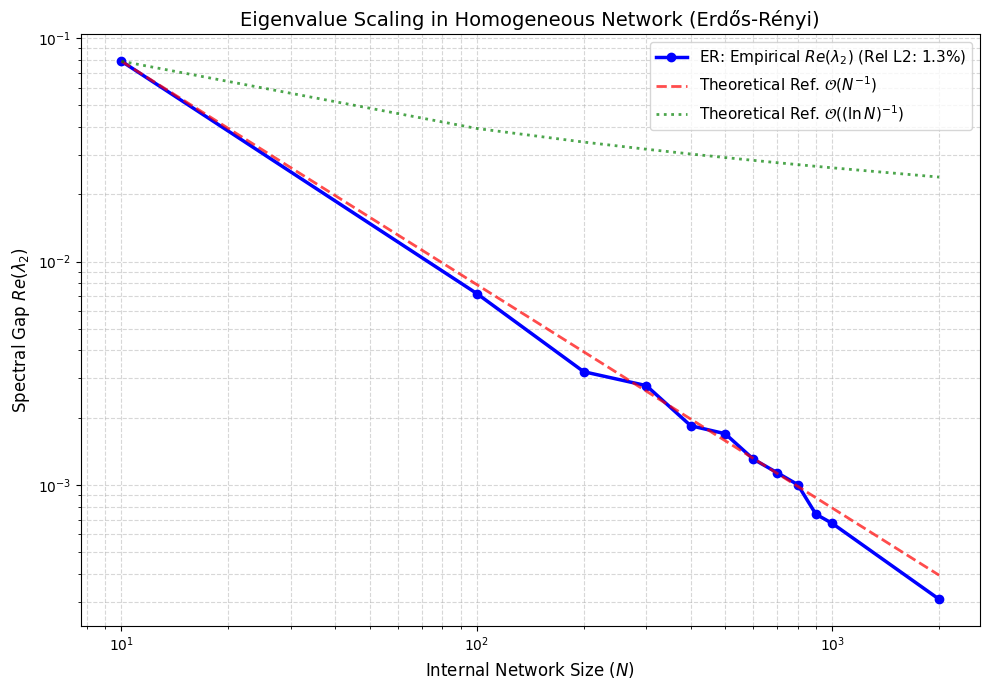
\includegraphics[width=\textwidth]{img/FH_model/ER_Network/Spectral_gap_ER.png}
        \caption{Scaling of the spectral gap $\text{Re}(\lambda_2)$ as a function of $N$ for the Erdős–Rényi (ER) topology, confirming the identical $\mathcal{O}(N^{-1})$ decay limit.}
        \label{fig:spectral_gap_er}
    \end{minipage}
\end{figure}

Therefore, to maintain a constant effective macroscopic coupling ($\sigma \text{Re}(\lambda_2) \approx \text{constant}$) and ensure that the operator learns a consistent continuous continuum limit regardless of the spatial discretization size $N$, the physical diffusion coefficient must systematically scale as $\sigma \propto N$.

%Let's focus on the case of the ER network. Here, since the connection probability is $p=\frac{3}{N}$ the average degree is fixed: $\lt k\gt = 3$.

For our experiments we chose $\sigma=0.1*N$.

%%%%%%%%%%%%%%%%%%%%%%%%%%%%%%%%%%%%%%%%
%REAL DATA
%%%%%%%%%%%%%%%%%%%%%%%%%%%%%%%%%%%%%%%%

\newpage
\section{Real data}
\subsection{The dataset}
After validating the Operator Learning approach on synthetic data generated by deterministic models (Hodgkin-Huxley and FitzHugh-Nagumo) and on complex networks, we now extend the analysis to real electrophysiological data.

The transition from the simulated to the biological domain introduces significant challenges. In synthetic models, the cause-and-effect relationship is well-defined: a known input current $I_{app}(t)$ produces a deterministic (or stochastic with controlled noise) voltage response. 

In real experimental data, however, the observed neuronal response is the result of the integration of multiple signals: not only the sensory stimulus controlled by the experimenter, but also feedback signals, the internal state of the animal, attention, preparatory motor activity, and intrinsic background noise. 

Consequently, the fundamental assumption of Operator Learning---namely, the existence of an operator $G: u \to v$ that uniquely maps a single input to the observed response---is a simplification. In this work, we will nevertheless assume this framework to be valid, treating the unobserved variables as stochastic noise that the neural network must filter out in order to learn the average dynamics induced by the stimulus.

%We now delve into the application of our machinery to a real neural system.
%In particular, we wanted to preserve the point of view of an emulation of an unknown underlying neural network.
The dataset employed in this work originates from the classic vibrotactile discrimination experiments conducted by Romo's group \cite{Romo_1999_Nature}.
The experiment consists of a working memory task performed by trained macaques. The protocol, termed \textit{two-alternative forced-choice} (2AFC), is structured into the following phases:
\begin{enumerate}
    \item \textbf{Stimulus 1 ($f_1$):} A probe vibrates on the monkey's fingertip at a frequency $f_1$ for 500 ms.
    \item \textbf{Delay:} A delay period (typically 3-6 seconds) during which no stimulus is presented. The monkey must maintain the memory trace of $f_1$.
    \item \textbf{Stimulus 2 ($f_2$):} A second vibration with frequency $f_2$ is presented for 500 ms.
    \item \textbf{Decision:} The monkey must indicate, by pressing one of two buttons, whether $f_2 > f_1$ or vice versa.
\end{enumerate}


\begin{figure}[htbp]
    \centering
    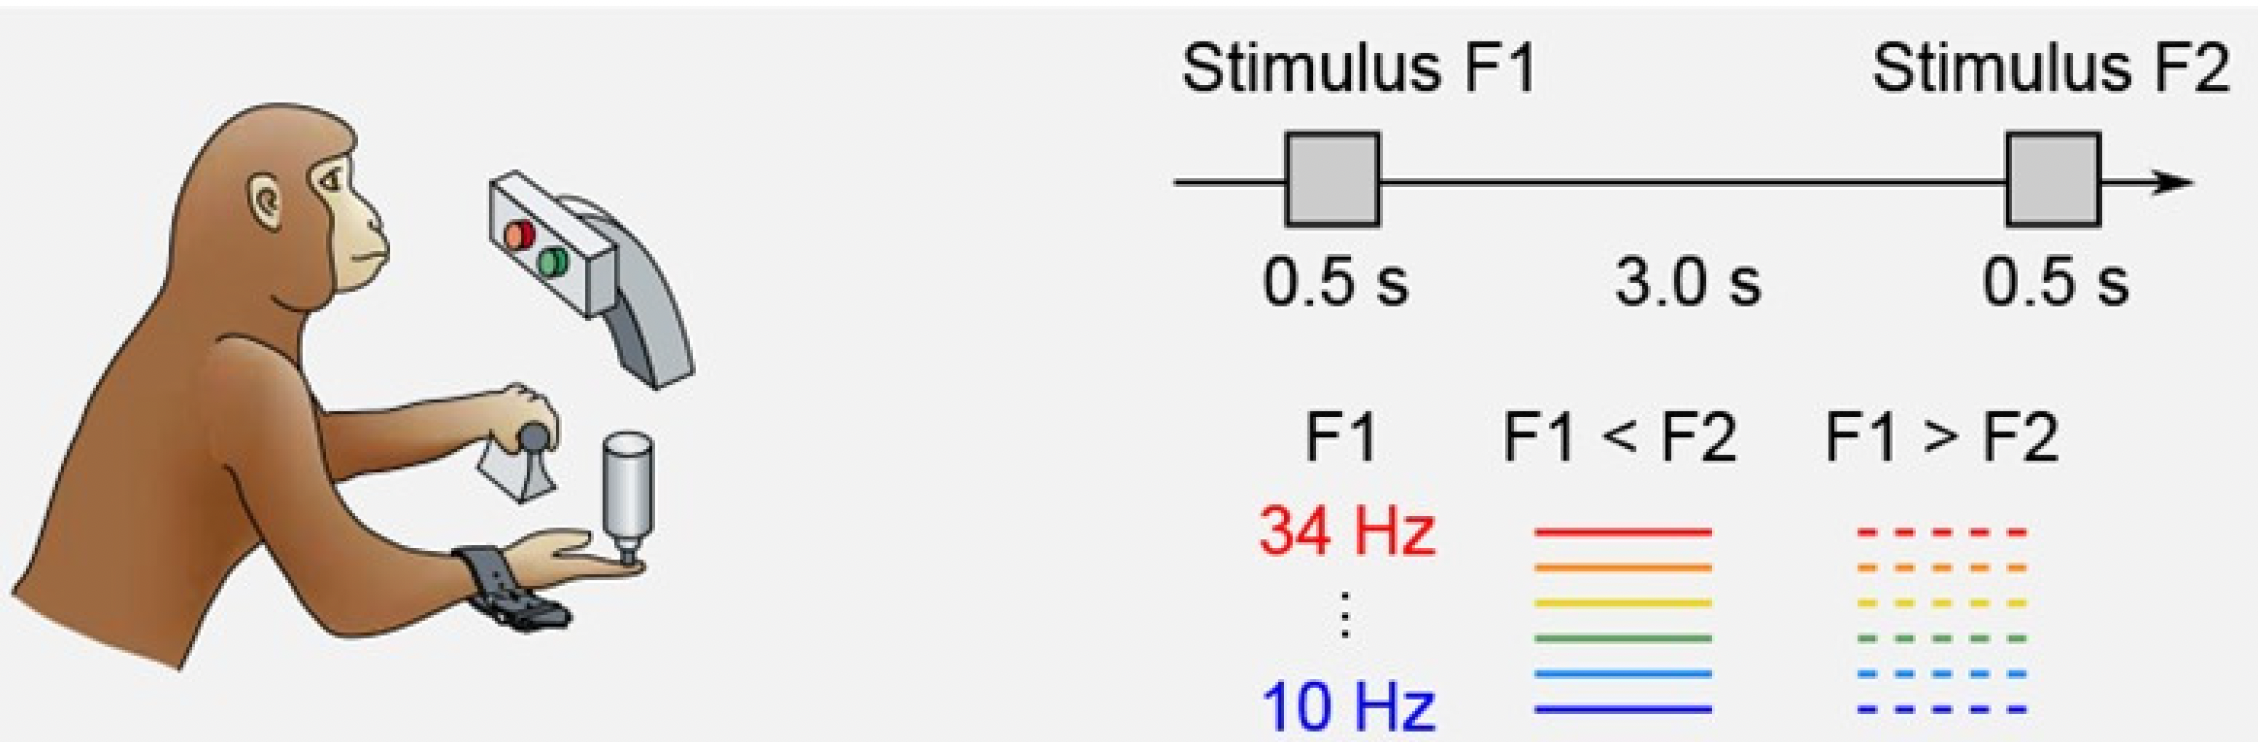
\includegraphics[width=0.85\textwidth]{img/Real_Data/Romo_task.png}
    \caption{Sequence of events in the vibrotactile two-alternative forced-choice (2AFC) task. The monkey perceives the first mechanical stimulus ($f_1$), maintains its trace in working memory during the delay period, and compares it against the second stimulus ($f_2$) to execute the motor decision.}
    \label{fig:romo_task}
\end{figure}

The possible choices for frequences $f_1$ and $f_2$ are {10,
14, 18, 26, 30, 34}.
Moreover, the data consist of extracellular recordings of individual neurons (Single Unit Activity) from the ventral prefrontal cortex (VPC), a crucial area for the maintenance of short-term memory and decision-making processes.

\subsection{First preprocessing}
The raw data consist of \textit{spike trains}, which are discrete temporal sequences indicating the exact moments a neuron generates an action potential. Since FNO (and in general Neural Operators) operate on continuous functions, a preprocessing step is required to transform these discrete events into continuous \textit{firing rates}.

The preprocessing involved the following steps:
\begin{enumerate}
    \item \textbf{Instantaneous Firing Rate Calculation:} The spike trains were convolved with a Gaussian kernel ($\sigma = 50$ ms) and sampled at $100$ Hz to obtain a continuous estimate of the firing probability density over time.
    \item \textbf{Time Warping and Alignment:} Since the duration of the experimental phases can vary slightly across trials, and the neuronal response can exhibit variable latencies, the data were temporally aligned (\textit{time-warped}) using a piecewise-linear transformation. Specifically, we defined key alignment events based on the task structure, such as the onset and offset of the first ($f_1$) and second ($f_2$) vibratory stimuli. Mathematically, let $t_i$ be the exact times of these specific events in a given trial, and $T_i$ be the median times of those same events computed across all trials. The instantaneous firing rate $x(t)$ was stretched or compressed along the time axis such that each trial-specific event $t_i$ was mapped precisely to the global median time $T_i$. This guarantees that the stimulus phases coincide perfectly across all samples, which is a crucial requirement to allow the neural network to learn consistent temporal patterns.
    \item \textbf{Filtering and Normalization:} To stabilize the variance and avoid numerical artifacts, neurons with atypically high mean firing rates (above $50$ Hz) were excluded from the dataset. Finally, the data matrix was mean-centered by subtracting the overall mean firing rate from the individual neural responses before further analysis. Moreover, since the overall error rate was 6\%, we analyzed only correct trials. 
\end{enumerate}

Figure \ref{fig:preprocessing_rates} shows an example of the preprocessed firing rates for different trials. The high trial-to-trial variability ("noise") typical of \textit{in vivo} recordings is clearly noticeable (in particular a correlation between stimulus and output is hardly noticeable), making the direct learning of the single-neuron dynamics with respect to the stimulus a highly challenging task.

\begin{figure}[H]
    \centering
    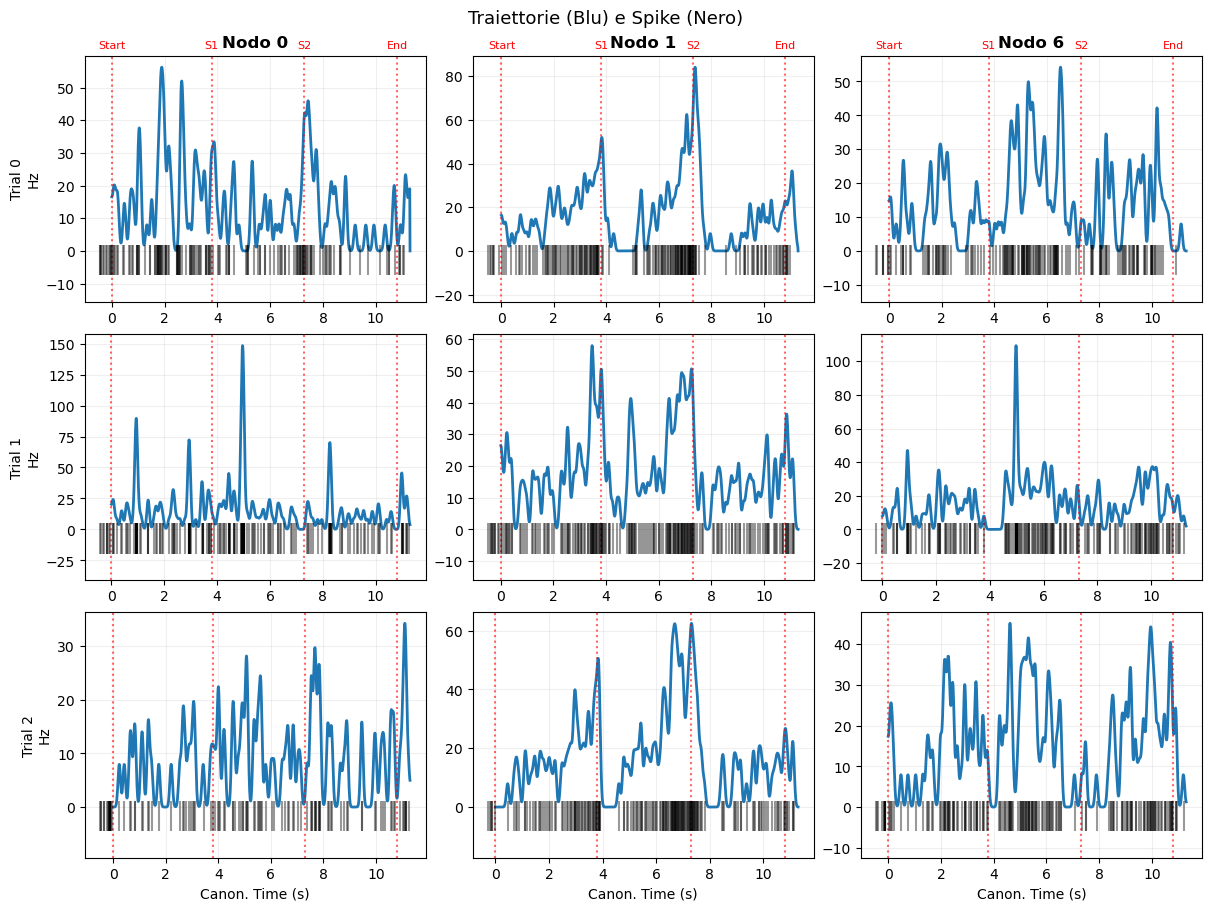
\includegraphics[width=0.8\textwidth]{img/Real_Data/Monkey_output_semi_raw.png}
    \caption{Example of preprocessed neuronal activity for a single neuron across multiple trials. The curves represent the \textit{warped firing rate}. Note the significant variability in the response even to the exact same stimulus, which is due to intrinsic noise and unobserved dynamics.}
    \label{fig:preprocessing_rates}
\end{figure}

\subsection{Second preprocessing: dPCA}
Given the noisy and high-dimensional nature of the population activity (hundreds of recorded neurons), training a neural operator on the single raw channels is highly ineffective. To extract the task-relevant latent dynamics, we applied \textbf{Demixed Principal Component Analysis (dPCA)} \cite{Kobak_2016_dPCA}.

Unlike standard PCA, which maximizes the total variance of the data without taking the experimental condition labels into account, dPCA decomposes the total variance into marginal components attributable to specific task parameters. In our case, given the neural activity tensor $\mathbf{X}$ (a multidimensional array containing the instantaneous firing rates of $N$ neurons across $S$ stimuli, $Q$ decisions, $K$ trials, and $T$ time points), the data variance is mathematically partitioned into five parts: condition-independent, stimulus-dependent, decision-dependent, stimulus-decision interaction, and trial-to-trial noise. 

dPCA seeks a transformation matrix that projects the data into a latent space where the meaningful components are "demixed", isolating:
\begin{itemize}
    \item \textbf{Condition-independent (Temporal) Component:} Captures the dynamics common to all trials, representing the general temporal evolution of the task irrespective of the condition.
    \item \textbf{Stimulus-dependent Component:} Captures the variations in neural activity that depend exclusively on the sensory stimulus (i.e., the values of the frequencies $f_1$ and $f_2$).
    \item \textbf{Decision-dependent Component:} Captures the variance related to the animal's choice or motor response.
    \item \textbf{Interaction Component:} Captures the variance arising from the non-linear interaction between the stimulus and the decision.
\end{itemize}

The trial-to-trial variability is treated mathematically as a \textbf{Noise} term in the variance decomposition, which the dPCA loss function is explicitly designed to penalize and filter out during the dimensionality reduction process.

Formally, the objective is to find a decoder matrix $\mathbf{D}$ and an encoder matrix $\mathbf{F}$ that minimize the reconstruction error evaluated on the data marginalizations \cite{Kobak_2016_dPCA}. For the implementation, we utilized the official library provided by the authors\footnote{Code available on GitHub: \url{https://github.com/machenslab/dPCA}}.

Mathematically, let $\mathbf{X}$ be the centered data matrix containing the single-trial instantaneous firing rates of all $N$ recorded neurons. The marginalization procedure decomposes this matrix into a sum of parameter-specific averages (the marginalizations) and a trial-to-trial noise term:
$$ \mathbf{X} = \sum_{\phi} \mathbf{X}_{\phi} + \mathbf{X}_{noise} $$
where $\phi$ iterates over the relevant task parameters (e.g., condition-independent time, stimulus, decision, and their interactions). Each term $\mathbf{X}_\phi$ captures the portion of the data variance exclusively attributable to that specific parameter.

The core objective of dPCA is to find a set of decoder matrices $\mathbf{D}_\phi$ and encoder matrices $\mathbf{F}_\phi$ for each marginalization $\phi$. The decoders linearly project the full neural activity $\mathbf{X}$ into a low-dimensional latent space, while the encoders map this latent representation back to reconstruct the parameter-specific target $\mathbf{X}_\phi$. These matrices are obtained by minimizing the following loss function:
$$ L = \sum_{\phi} L_{\phi} = \sum_{\phi} ||\mathbf{X}_{\phi} - \mathbf{F}_{\phi} \mathbf{D}_{\phi} \mathbf{X}||^{2} $$

In experimental scenarios with unbalanced data (e.g., varying number of trials per condition, aborted trials, or self-paced tasks), this formulation is adapted to operate on trial-averaged firing rates (PSTHs), denoted as $\tilde{\mathbf{X}}$. By introducing a regularization parameter $\mu$ to prevent overfitting and a noise covariance matrix $\tilde{\mathbf{C}}_{noise}$, the objective function for each component is adjusted to:
$$ L_{\phi} = ||\tilde{\mathbf{X}}_{\phi} - \mathbf{F}_{\phi} \mathbf{D}_{\phi} \tilde{\mathbf{X}}||^{2} + SQT ||\mathbf{F}_{\phi} \mathbf{D}_{\phi} \tilde{\mathbf{C}}_{noise}^{1/2}||^{2} + \mu ||\mathbf{F}_{\phi} \mathbf{D}_{\phi}||^{2} $$
where $S$, $Q$, and $T$ represent the number of stimuli, decisions, and time points, respectively. This optimization problem amounts to a Reduced-Rank Regression (RRR) and can be efficiently solved analytically via Singular Value Decomposition (SVD).

For the training of our Neural Operator, we specifically selected the projection of the test set onto the decoder axis $\mathbf{d}$ corresponding to the \textit{first stimulus component}. This provides a one-dimensional, continuous latent trajectory $u(t)$ that represents the "pure response" of the neural network to the vibrotactile stimulus, efficiently filtered from noise and non-pertinent dynamics.

\begin{figure}[htbp]
    \centering
    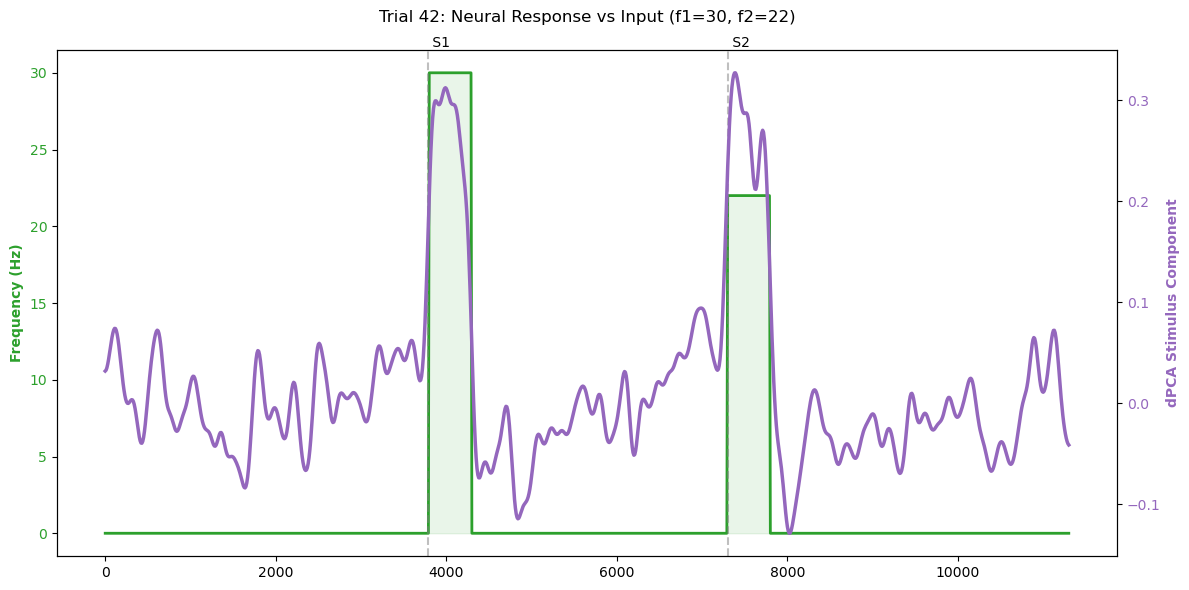
\includegraphics[width=\textwidth]{img/Real_Data/Monkey_dPCA.png}
    \caption{First stimulus dPCA component for an exemplary trial ($f_1 = 30$ Hz, $f_2 = 22$ Hz). The solid green line represents the applied stimulus frequency (left axis), while the solid purple line displays the corresponding projection of the population activity onto the first stimulus-dependent dPCA axis (right axis). Note how the latent neural trajectory reflects the stimulus presentation phases.}
    \label{fig:monkey_dpca_stimulus}
\end{figure}


\subsubsection{Comparison: PCA vs dPCA}

To better understand the advantage of dPCA, it is useful to compare it with standard Principal Component Analysis (PCA) and Linear Discriminant Analysis (LDA), as illustrated in Figure \ref{fig:pca_vs_dpca}.

Standard PCA is an unsupervised dimensionality reduction technique. It compresses the data by finding orthogonal axes (principal components) that maximize the explained variance and minimize the overall reconstruction error. However, because it is entirely blind to the experimental task parameters, the resulting components often exhibit mixed selectivity. Consequently, the temporal dynamics, stimulus information, and decision variables remain entangled within the same latent projections (Figure \ref{fig:pca_vs_dpca}c, d).

Conversely, LDA is a supervised method explicitly designed to find an axis that maximally separates different classes (e.g., different stimuli). While LDA perfectly demixes the task parameters, it does not attempt to preserve the original geometry of the data or minimize the reconstruction error, often leading to a distorted representation of the underlying neural population dynamics (Figure \ref{fig:pca_vs_dpca}a, b).

dPCA bridges the gap between these two approaches. By explicitly partitioning the data variance into marginalizations based on the task parameters (Figure \ref{fig:pca_vs_dpca}g), dPCA enforces a demixing constraint. Crucially, it gains additional flexibility by utilizing separate decoder and encoder matrices ($\mathbf{D}$ and $\mathbf{F}$). The decoder projects the data onto an axis that separates the task parameters (similar to LDA), while the encoder reconstructs the original class means, thereby preserving the structural geometry and minimizing the reconstruction error (similar to PCA) (Figure \ref{fig:pca_vs_dpca}e, f, h).

\begin{figure}[htbp]
    \centering
    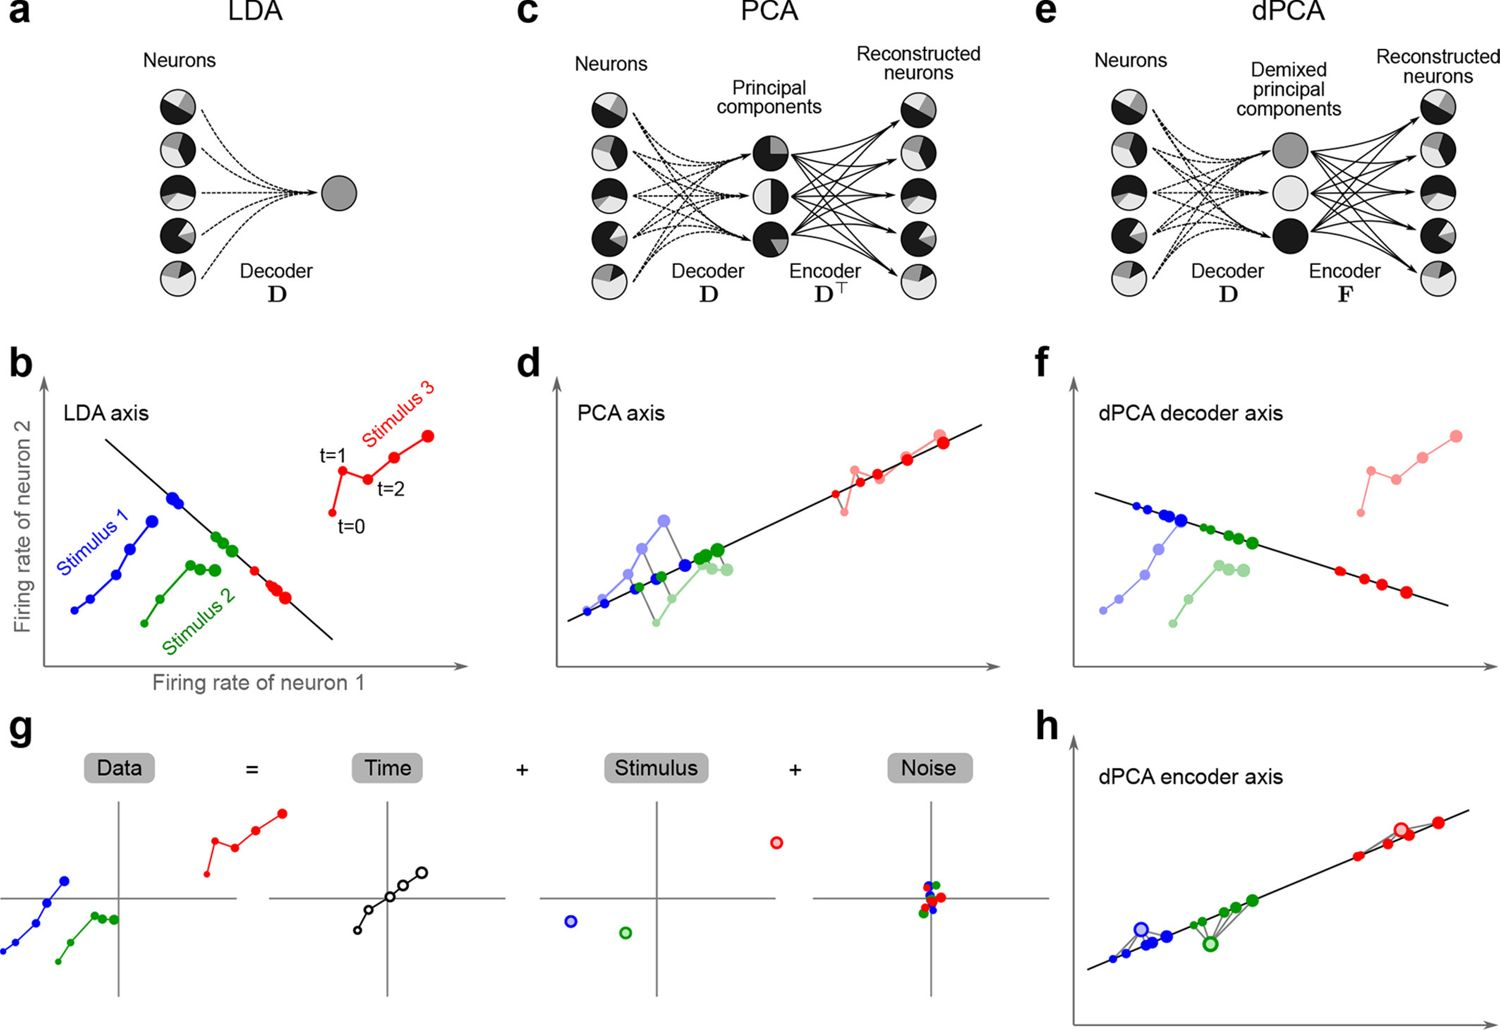
\includegraphics[width=\textwidth]{img/Real_Data/PCA vs dPCA.jpg}
    \caption{Comparison of Linear Discriminant Analysis (LDA), Principal Component Analysis (PCA), and demixed Principal Component Analysis (dPCA). (a, b) LDA separates the classes but distorts the geometric distances between them. (c, d) PCA accurately reconstructs the data and preserves distances but mixes the task parameters. (e-h) dPCA utilizes separate decoder and encoder matrices to effectively demix the task parameters while simultaneously preserving the original data geometry and minimizing reconstruction error.}
    \label{fig:pca_vs_dpca}
\end{figure}

\newpage
\subsection{Results with FNO}

In this section, we present the results of applying the Fourier Neural Operator (FNO) to learn the mapping from the sensory input to the latent neural dynamics. The input to the network was modeled as a simple square wave function: its amplitude represents the frequency of the applied vibrotactile stimulus, and its non-zero width corresponds to the true duration of the signal. The target output during training was the first stimulus-dependent latent trajectory extracted via dPCA, as described in the previous section.

Figure \ref{fig:fno_latent_results} illustrates the performance of the FNO in the latent space. Considering that the network is tasked with reproducing an entire, complex stimulus-driven neural dynamics from merely two macroscopic parameters (stimulus frequency and duration), the fits are remarkably accurate. The FNO successfully captures the transient peaks, the latency of the response, and the overall temporal evolution of the latent trajectory.

\begin{figure}[htbp]
    \centering
    \begin{subfigure}[b]{0.8\textwidth}
        \centering
        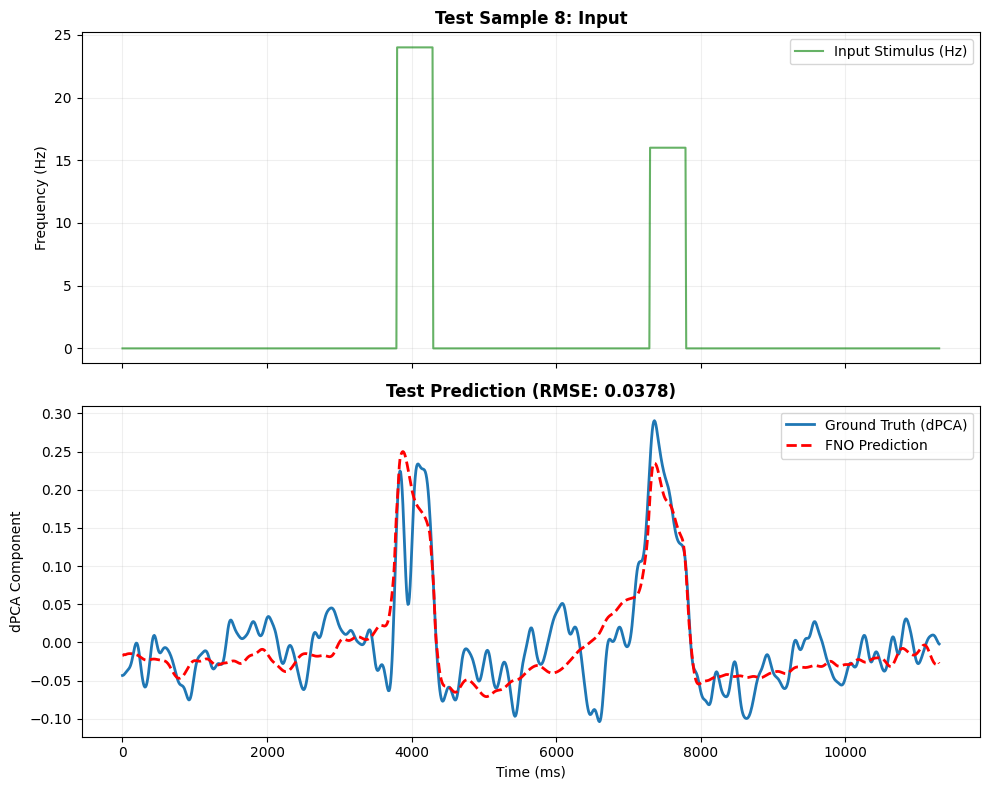
\includegraphics[width=\textwidth]{img/Real_Data/monkey_test_figure.png}
        \caption{Example of FNO prediction vs Ground Truth (1st stimulus dPC) for a test sample.}
    \end{subfigure}
    
    \vspace{0.4cm}
    
    \begin{subfigure}[b]{0.8\textwidth}
        \centering
        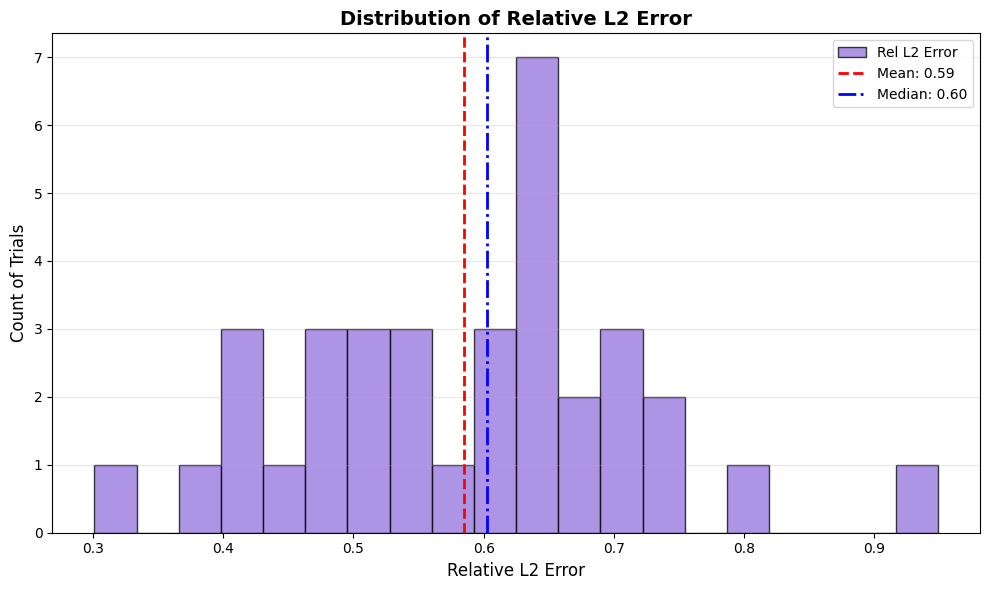
\includegraphics[width=\textwidth]{img/Real_Data/monkey_hist_test_set.png}
        \caption{Distribution of the relative $L_2$ error across the entire test set.}
    \end{subfigure}
    \caption{Performance of the FNO in predicting the latent stimulus dynamics.}
    \label{fig:fno_latent_results}
\end{figure}

To evaluate the predictive power of the model in the original physiological space, we performed the inverse transformation. This involved applying the inverse dPCA (multiplying the latent predictions by the corresponding encoder matrix $\mathbf{F}$) and subsequently reversing the time-warping procedure (de-warping) to restore the original trial timeframes. 

However, evaluating the model by reconstructing the total firing rate presents a visualization challenge. If we add back all the other marginalized components (such as the condition-independent baseline, decision, and interaction components) to our predicted stimulus component, the differences between the FNO prediction and the ground truth become virtually imperceptible. This occurs because the variance of the stimulus component is drastically smaller than the overall baseline and condition-independent activity (Figure \ref{fig:reprojection_total}). The stimulus-induced modulations are "masked" by the dominant task-general dynamics.

\begin{figure}[htbp]
    \centering
    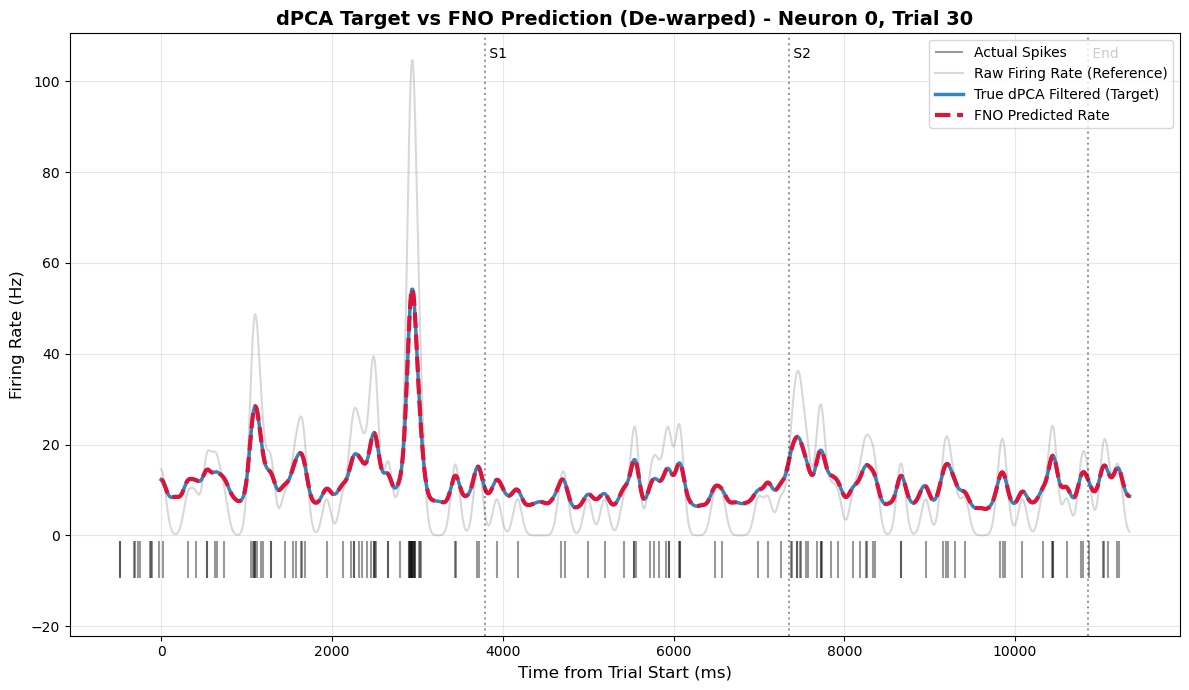
\includegraphics[width=0.9\textwidth]{img/Real_Data/Reprojection (total).png}
    \caption{Total reconstructed firing rate for a sample neuron (Neuron 0). When the predicted stimulus component is added back to the other task marginalizations, the overall predicted rate (dashed red line) almost perfectly overlaps the target (solid blue line), masking the specific contribution of the FNO due to the large scale of the condition-independent baseline.}
    \label{fig:reprojection_total}
\end{figure}

Therefore, a much more informative way to assess the FNO's performance in the direct space is to isolate and compare \textit{only} the pure stimulus component for individual neurons, ignoring the other marginalizations. 

Figure \ref{fig:reprojection_stimulus} shows this direct-space comparison for Neuron 8. This specific neuron was selected because it possesses the highest absolute weight in the encoder matrix corresponding to the first stimulus dPC. In biological terms, Neuron 8 is the unit within the recorded population that responds most strongly to the stimulus variations. The plot demonstrates that the FNO is highly capable of predicting the specific, real-space firing rate modulations induced by the vibrotactile stimuli, correctly locating the peaks corresponding to the $f_1$ and $f_2$ stimulation phases.

\begin{figure}[htbp]
    \centering
    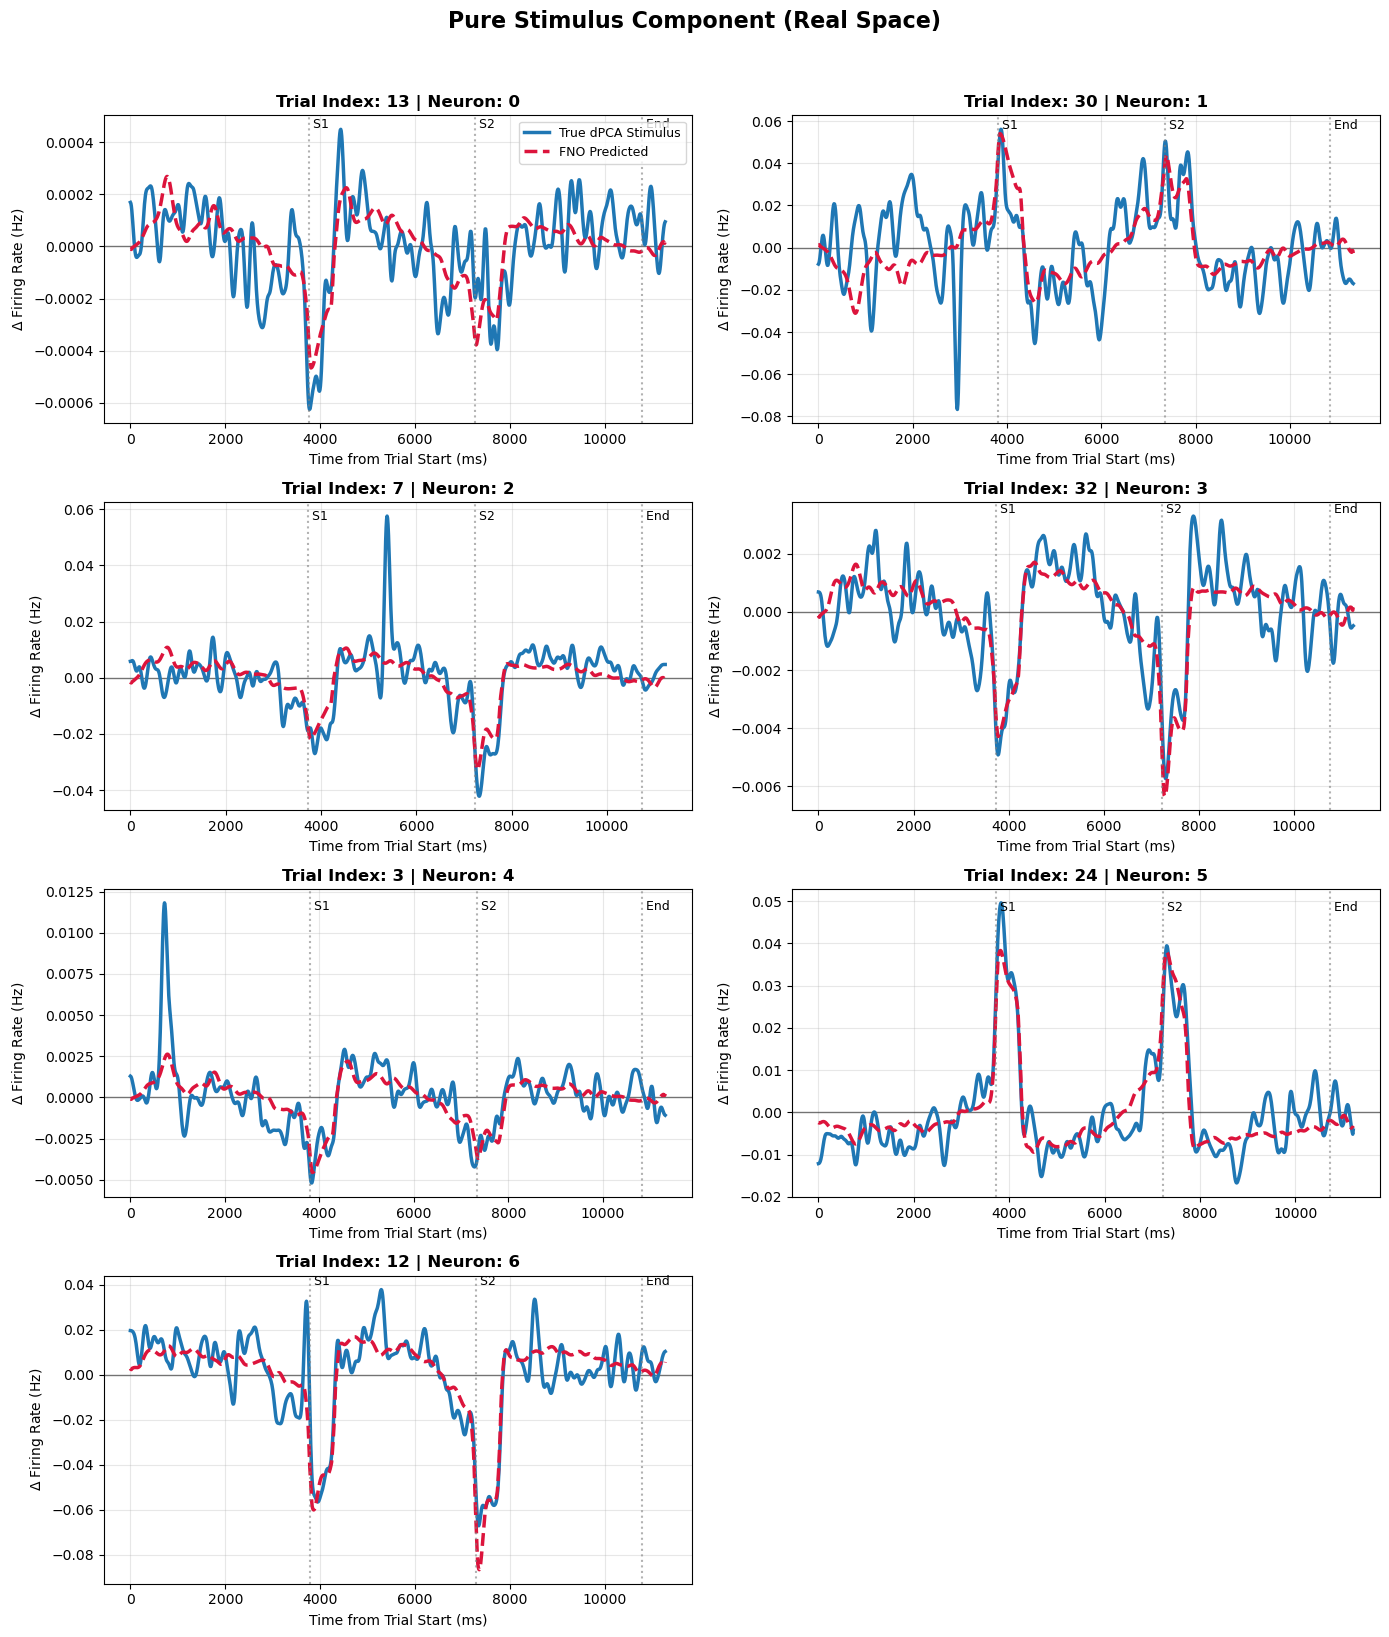
\includegraphics[width=0.9\textwidth]{img/Real_Data/Reprojection (stimulus) - multiple.png}
    \caption{Pure stimulus component in real space for Neuron 8 (the neuron with the highest encoder weight for the stimulus dPC). By isolating the stimulus effect from the overall baseline, we can clearly observe how well the FNO predicts the actual firing rate modulations during the $S_1$ and $S_2$ presentation windows.}
    \label{fig:reprojection_stimulus}
\end{figure}

\begin{table}[htbp]
\centering
\caption{dPCA Encoder weights for the first stimulus component ($f_1, f_2$). Neuron 1 exhibits the largest absolute weight, indicating the strongest firing rate modulation in response to the stimulus.}
\label{tab:encoder_weights}
\begin{tabular}{|l|c|}
\hline
\textbf{Neuron} & \textbf{Encoder Weight} \\ \hline
Neuron 0        & -0.0036                     \\
\textbf{Neuron 1} & \textbf{0.4141}           \\
Neuron 2        & -0.1695                     \\
Neuron 3        & -0.0273                     \\
Neuron 4        & -0.0349                     \\
Neuron 5        & 0.1287                      \\
Neuron 6        & -0.2490                     \\ \hline
\end{tabular}
\end{table}